% -*- Mode: Latex; -*-
% ------------------------------------------------------------------------
% Default style
% ------------------------------------------------------------------------

% If arxiv-style, comment below line

%\def\useorstyle{1}
\ifdefined\useorstyle
\documentclass{article}
\pdfoutput=1

%\documentclass[opre,blindrev]{informs3} % current default for manuscript submission
\usepackage[numbers]{natbib} 
%\usepackage{macros/neurips_2023}
\usepackage{macros/nips_2024}

\usepackage{macros/statistics-macros}
\usepackage{macros/packages}
\usepackage{macros/editing-macros}
\usepackage{macros/formatting}
\usepackage{macros/statistics-macros}
\usepackage{caption}
%\DoubleSpacedXI % Made default 4/4/2014 at request
%%\OneAndAHalfSpacedXI % current default line spacing
%%\OneAndAHalfSpacedXII 
%%\DoubleSpacedXII

% If hyperref is used, dvi-to-ps driver of choice must be declared as
%   an additional option to the \documentclass. For example
%\documentclass[dvips,opre]{informs3}      % if dvips is used 
%\documentclass[dvipsone,opre]{informs3}   % if dvipsone is used, etc. 

%%% OPRE uses endnotes
\usepackage{endnotes}
\let\footnote=\endnote
\let\enotesize=\normalsize
\def\notesname{Endnotes}%
\def\makeenmark{\hbox to1.275em{\theenmark.\enskip\hss}}
\def\enoteformat{\rightskip0pt\leftskip0pt\parindent=1.275em
  \leavevmode\llap{\makeenmark}}
\usepackage{xspace}
% Private macros here (check that there is no clash with the style)

% Natbib setup for author-year style
% \usepackage{natbib}
%  \bibpunct[, ]{(}{)}{,}{a}{}{,}%
%  \def\bibfont{\small}%
%  \def\bibsep{\smallskipamount}%
%  \def\bibhang{24pt}%
%  \def\newblock{\ }%
%  \def\BIBand{and}%

%% Setup of theorem styles. Outcomment only one. 
%% Preferred default is the first option.
%\TheoremsNumberedThrough     % Preferred (Theorem 1, Lemma 1, Theorem 2)
%\TheoremsNumberedByChapter  % (Theorem 1.1, Lema 1.1, Theorem 1.2)
%\ECRepeatTheorems

%% Setup of the equation numbering system. Outcomment only one.
%% Preferred default is the first option.
%\EquationsNumberedThrough    % Default: (1), (2), ...
%\EquationsNumberedBySection % (1.1), (1.2), ...

% In the reviewing and copyediting stage enter the manuscript number.
%\MANUSCRIPTNO{} % When the article is logged in and DOI assigned to it,
                 %   this manuscript number is no longer necessary
 

% \usepackage{fullpage}
\usepackage{hyperref}

% \usepackage{setspace}
\usepackage{pgfplotstable}
\usepackage{graphicx}
% \usepackage{subcaption}
\usepackage{float} 
\usepackage{tabularx}
\usepackage{overpic}
\usepackage{tikz}
\usepackage{rotating}
\usepackage{psfrag}
\usepackage{enumitem}
\usepackage{tikz}
\usetikzlibrary{shapes, arrows, positioning}  


%%%%%%%%%%%%%%%%
%\begin{document}
%%%%%%%%%%%%%%%%

% Outcomment only when entries are known. Otherwise leave as is and
%   default values will be used.
%\setcounter{page}{1}
%\VOLUME{00}%
%\NO{0}%
%\MONTH{Xxxxx}% (month or a similar seasonal id)
%\YEAR{0000}% e.g., 2005
%\FIRSTPAGE{000}%
%\LASTPAGE{000}%
%\SHORTYEAR{00}% shortened year (two-digit)
%\ISSUE{0000} %
%\LONGFIRSTPAGE{0001} %
%\DOI{10.1287/xxxx.0000.0000}%

% Author's names for the running heads
% Sample depending on the number of authors;
% \RUNAUTHOR{Jones}
% \RUNAUTHOR{Jones and Wilson}
% \RUNAUTHOR{Jones, Miller, and Wilson}
% \RUNAUTHOR{Jones et al.} % for four or more authors
% Enter authors following the given pattern:
%\RUNAUTHOR{}

% Title or shortened title suitable for running heads. Sample:
% \RUNTITLE{Bundling Information Goods of Decreasing Value}
% Enter the (shortened) title:
% \RUNAUTHOR{Che and Namkoong}
% \RUNTITLE{Adaptive Experimentation at Scale}

% Full title. Sample:
% \TITLE{Bundling Information Goods of Decreasing Value}
% Enter the full title:
\title{A Planning Framework for Adaptive Labeling}
 
% Block of authors and their affiliations starts here:
% NOTE: Authors with same affiliation, if the order of authors allows,
%   should be entered in ONE field, separated by a comma.
%   \EMAIL field can be repeated if more than one author
 
%  \AUTHOR{Daksh Mittal}
% \AFF{Decision, Risk, and Operations Division, Columbia Business School, New York, NY 10027, \EMAIL{namkoong@gsb.columbia.edu}} %, \URL{}}

% \AUTHOR{Yuanzhe Ma}

% \AUTHOR{Shalmali Joshi}


% \AUTHOR{Hongseok Namkoong}
% \AFF{Decision, Risk, and Operations Division, Columbia Business School, New York, NY 10027, \EMAIL{namkoong@gsb.columbia.edu}} %, \URL{}}

 
\date{\today}
%\author{}
% Sample
%\KEYWORDS{deterministic inventory theory; infinite linear programming duality;
%  existence of optimal policies; semi-Markov decision process; cyclic schedule}

% Fill in data. If unknown, outcomment the field
% \KEYWORDS{adaptive experimentation, A/B testing, experimental design}
% \HISTORY{This paper was first submitted on July,
%   2020.}

\maketitle
%%%%%%%%%%%%%%%%%%%%%%%%%%%%%%%%%%%%%%%%%%%%%%%%%%%%%%%%%%%%%%%%%%%%%%

% Samples of sectioning (and labeling) in MNSC
% NOTE: (1) \section and \subsection do NOT end with a period
%       (2) \subsubsection and lower need end punctuation
%       (3) capitalization is as shown (title style).
%
%\section{Introduction.}\label{intro} %%1.
%\subsection{Duality and the Classical EOQ Problem.}\label{class-EOQ} %% 1.1.
%\subsection{Outline.}\label{outline1} %% 1.2.
%\subsubsection{Cyclic Schedules for the General Deterministic SMDP.}
%  \label{cyclic-schedules} %% 1.2.1
%\section{Problem Description.}\label{problemdescription} %% 2.

% Text of your paper here

\else

\documentclass[11pt]{article}
\usepackage[numbers]{natbib}
%\usepackage[nonatbib]{neurips_2024}
\usepackage{macros/packages}
\usepackage{macros/editing-macros}
\usepackage{macros/formatting}
\usepackage{macros/statistics-macros}
 

% \onehalfspacing
% \renewcommand{\baselinestretch}{1.35}

% \title{Adaptive Labeling for Efficient Out-of-distribution Model Evaluation}


\begin{document}
%\maketitle

% Control whitespace around equations
\abovedisplayskip=8pt plus0pt minus3pt
\belowdisplayskip=8pt plus0pt minus3pt


% ------------------------------------------------------------------------
% Main Paper Body
% ------------------------------------------------------------------------


% ------------------------------------------------------------------------
% Default title and authorship
% ------------------------------------------------------------------------
\begin{center}
  {\huge A Planning Framework for Adaptive Labeling\footnote{
  A conference version of this work appeared at 
2024 Conference on Neural Information Processing Systems,
titled 
``Adaptive Labeling for Efficient Out-of-distribution Model Evaluation''.}} \\
  \vspace{.5cm}
  {\Large Daksh Mittal$^{*1}$~~  Yuanzhe Ma$^{*2}$ ~~
  Shalmali Joshi$^{3}$ ~~ Hongseok Namkoong$^{1}$
  } \\
{ Decision, Risk, and Operations Division$^{1}$,
  Department of Industrial Engineering and Operations Research$^{2}$,
  Department of Biomedical Informatics$^{3}$ \\
  Columbia University
  } \\ 
\end{center}

% ------------------------------------------------------------------------
% Abstract
% ------------------------------------------------------------------------



\fi
%\linenumbers

\def\thefootnote{*}\footnotetext{Equal contribution}
%\def\thefootnote{\arabic{footnote}}

\begin{abstract}
\begin{abstract}
Retrieval-Augmented Generation (RAG) is often used with Large Language Models (LLMs) to infuse domain knowledge or user-specific information. In RAG, given a user query, a retriever extracts chunks of relevant text from a knowledge base. These chunks are sent to an LLM as part of the input prompt. Typically, any given chunk is repeatedly retrieved across user questions. However, currently, for every question, attention-layers in LLMs fully compute the key values (KVs) repeatedly for the input chunks, as state-of-the-art methods cannot reuse KV-caches when chunks appear at arbitrary locations with arbitrary contexts. Naive reuse leads to output quality degradation.  This leads to potentially redundant computations on expensive GPUs and increases latency. In this work, we propose \sys, a system for managing and reusing precomputed KVs corresponding to the text chunks (we call \textit{chunk-caches}) in RAG-based systems. We present how to identify \hl{\textit{chunk-caches} that are reusable}, how to efficiently perform a small fraction of recomputation to \textit{fix} the cache to maintain output quality, and how to efficiently store and evict \textit{chunk-caches} in the hardware for maximizing reuse while masking any overheads. With real production workloads as well as synthetic datasets, we show that \sys reduces redundant computation by \textbf{51\%} over SOTA prefix-caching and \textbf{75\%} over full recomputation.
\hl{Additionally, with continuous batching on a real production workload, we get a \textbf{1.6$\times$} speedup in throughput and a \textbf{2$\times$} reduction in end-to-end response latency over prefix-caching while maintaining quality, for both the \llama-3-8B and \llama-3-70B models. 
}
\end{abstract}





\end{abstract}

\documentclass[../main.tex]{subfiles}
\graphicspath{{../images/}}
\makeatletter
\def\input@path{{../images/}}
\makeatother
\begin{document}
\section{Introduction}
\begin{figure}
\centering
\begin{tikzpicture}
\node[inner sep=0pt] (ws) at (0, 0) {
\includegraphics[height=.4\textwidth, trim={10cm 0 10cm 0},clip]{world_space.png}};
\node[inner sep=0pt] (cs) at (6,0) {\includegraphics[height=.4\textwidth, trim={10cm 1cm 10cm 4cm},clip]{conf_space.png}};
\end{tikzpicture}
\vspace{-5pt}
\label{fig:pbrm_intro}
\caption{\textbf{Left}: Shows world space obstacles as grey spheres. Robots start and goal configuration is colored red and green, respectively. Configurations along the computed path are colored transparent blue. \textbf{Right:} Mapped world space scenario to configuration space. Obstacle region is the grey mesh. Red spheres are collision-free regions computed by the neural SCDF. The optimized shortest path in the convex corridor is the blue curve.}
\vspace{-25pt}
\end{figure}
Motion planning is the problem of finding a collision-free trajectory that connects a given start and goal configuration. The planning takes place in the configuration space of the robot. For single body robots, like mobile robots or drones, the configuration space and the world space are usually the same. This simplifies the planning, since explicit obstacle representations are available which enables geometrical tools like separating hyperplanes, smallest distance to obstacles etc., to be used when designing motion planning algorithms. For multi-body robots like manipulators, the situation is completely different. The world space obstacles are usually mapped to non-convex regions, and to make the problem even harder, the mapping is usually not known. Forming explicit representations of the obstacle region in the configuration space is usually too expensive or intractable. Despite all of this, sampling based planners are used with great success, which mainly is due to their use of implicit representations of the obstacle region. The basic idea is to construct a graph in the configuration space that covers and connects the collision-free region. From this graph, a path can be extracted that connects a given start and goal configuration. The approach is computationally expensive, since the graph is constructed with the smallest geometrical building block available, points, which represents a collision-check. Furthermore, the extracted paths from the graph are non-smooth and jagged due to the stochastic nature of the approach. This adds an additional post-processing step to the process, where the paths are shortcutted and smoothened, before the path can be used for tracking. Clearly a lot of time is invested to form this graph and produce smooth paths. Thus, if the obstacles start to move, then all of this work is done in no use, since all points that make up this graph need to be re-verified, which is simply too time consuming to be done in real time.
\\\\
In this work, we want to address the existing drawbacks of the sampling based planners. Our main contribution is an improved motion planner where each vertex in the graph covers a collision-free region in the form of a sphere instead of a point and where the edges are formed with neighboring intersecting spheres. This representation has the advantage of instead of returning piecewise linear paths, returning a sequence of overlapping spheres, i.e. a convex corridor, that connects a given start and goal configuration, illustrated in Figure \ref{fig:pbrm_intro}. This convex corridor allows us to use convex optimization to produce smooth trajectories, instead of computationally expensive post-processing methods. The representation further allows us to estimate the coverage of the collision-free space, which gives us awareness and feedback in the offline roadmap construction phase. Finally, our representation is simple to adapt to moving obstacles, simply requery for the new radii and recheck for intersections. 
\\\\
The spherical collision-free regions are formed using a signed distance function (SDF), which is a function that returns the smallest distance from an arbitrary point to the boundary of an obstacle. As the name implies, the distance is signed, thus if the point is inside the obstacle it is negative otherwise positive. If the distance is positive, a sphere with radius equal to the distance is guaranteed to cover a collision-free region. Using an SDF in motion planning is not new, but what is novel about our approach is that we express the distance in the configuration space instead of the world space and by doing so allows us to form these convex collision-free regions. We refer to the resulting SDF as a signed configuration distance function (SCDF). Computing an SCDF analytically is non-trivial, our approach is therefore to parameterize the SCDF with a deep neural network and learn the mapping by supervised learning. Our resulting neural SCDF can compute distances for different parameter values of obstacle shapes and we also show how multiple distances can be combined, thus making our approach flexible.
\section{Related work}
Motion planning algorithms can roughly be divided into three families, grid-based, sampling based and optimization based methods. Grid-based methods (GBM) discretize the planning space from which a graph is then compiled. A standard search method is A$^\star$ \citep{a_star}, which is classified as an \textit{informed} search method, since it employs a heuristic function to speed up the search. A$^\star$ guarantees to return an optimal path at the level of discretization used. GBMs usually discretize the planning space by a regular lattice and this limits the GBMs to problems with low dimensionality due to the curse of dimensionality. Thus, GBMs are usually limited to single-body robots where the degrees of freedom (DOF) are low. To overcome the inherent scaling problem with the GBMs, stochastic methods are usually used for multi-body robots. These methods are termed as sampling-based methods (SBM) and core members within this family are the rapidly-exploring random trees (RRT) \citep{rrt} and the probabilistic roadmap (PRM) \citep{prm}. RRT grows a tree from the start configuration and explores the collision-free region in a rapid way until it is able to connect to the goal region. RRT is usually improved by bi-directional planning \citep{rrt_connect}, i.e. an additional tree is grown from the goal configuration and the trees are tested for connection after any tree has been expanded. RRT is a single-query method, thus it searches for a path from scratch each time it is queried. Contrary to this, PRM is a multi-query method, which solves for multiple queries without starting from scratch. PRM does this by creating a roadmap (graph) that covers the collision-free space as an offline step. The graph is then used to solve for multiple queries. PRMs are used in cases where the environment does not change since the extra offline step is too computationally costly and needs to be re-done if the environment is changed. In our work, we address this inherent issue by using a different roadmap representation. Our vertices in the graph cover a collision-free region in the form of spheres and we form the edges by checking for intersecting spheres. If something in the environment changes, we recompute the spheres radii and recheck the intersections, without relying on collision detection. We use a trained neural network to compute the sphere radius, therefore querying for the radius can be done fast, hence our representation enables the PRM for dynamic environments.
\\\\
In the recent decades, optimization based methods (OBM) \citep{chomp, schulman, itomp, stomp} have been introduced as an alternative to SBM for multi-body robots. Like the SBM, the OBMs scale well to higher dimensional problems and produce smoother motion. It is common to use a SDF in the optimization since it is a smooth function, thus enabling gradient-based methods. However, the standard way of expressing the SDF is in world space. The distance therefore needs to be mapped to the configuration space by the forward kinematics. This mapping makes the optimization problem a non-linear program (NLP), which is computationally expensive to solve. Recently, a different approach has been proposed. In \cite{mp_gcs} motion planning is formulated as a convex optimization problem by using the graph of convex sets framework \citep{gcs}. The underlying idea is to decompose the collision-free space into intersecting convex sets from which a convex optimization problem is formulated. In cases where an explicit representation of the obstacles in the configuration space exists, like for single-body robots, creating collision-free convex regions can be done fast \citep{iris}. For multi-body robots, this is non-trivial. Existing work does this successfully \citep{iris_nlp, iris_c} by an optimization based approach, but the methods are still too time consuming to be used in the presence of moving obstacles. Our approach is instead to use deep learning to learn an SDF expressed in the configuration space. With this, we can query for shortest distances to the collision boundary, which allows us to expand spherical regions which are collision-free. Our approach is fast and therefore enables our suggested roadmap planner to be used in dynamic environments.
\\\\
Recent research has focused on learning collision detection \citep{fk_kernel_distance, diffco, graphdistnet} by predicting the signed distance between the robot links and the surrounding obstacles in the world space. The learned SDF is used in trajectory optimization but since the distance is expressed in the world space, the problem becomes an NLP and therefore takes a long time to solve. We take a novel approach and suggest to instead express the signed distance in the configuration space. This allows us to improve the PRM at the same time as it enables convex optimization for trajectory optimization, which runs faster and is more reliable than NLP solvers. In \cite{cspf} a learned signed distance function in the configuration space is proposed similar to our approach. However, their approach is restricted to point cloud representations, while we propose to represent the obstacles as parameterized geometric shapes, e.g. spheres. Furthermore, we also show how to use our learned SCDF to improve an existing roadmap planner.
\section{Problem formulation}
A robot is located in the world space, $\W \subset \R^3 $. The unique location of the robot is given by its configuration $\q \in \C$, where $\C$ is the configuration space. The set of points covered by the robots bodies at a certain configuration is expressed as $\B(\q) \subset \W$. The robot is surrounded by $\NrObst$ obstacles $\O = \bigcup_{i=1}^{\NrObst} \O_i$, where  $\O_i \subset \W$. The representation of the obstacle in the configuration space is the set $\C\O_i = \{\q \in \C \: |\: \B(\q) \cap \O_i \neq \emptyset \}$. The obstacle space is formed as $\Co = \bigcup_{i=1}^{\NrObst} \C \O_i$. The complement is referred to as the free space, $\Cf = \C \setminus \Co$. The path planning problem is a tuple, ($\Cf$, $\qStart$, $\qGoal$), where we want to connect a query pair, consisting of a start, $\qStart$, and goal configuration, $\qGoal$, with a geometric path, $\q(s): [0, 1] \mapsto \Cf$, such that $\q(0)=\qStart$ and $\q(1)=\qGoal$, or report correctly when such a path does not exist.
\end{document}

\section{Related Work}
% \subsection{Vision Language Model}
% 시각장애인에서 상황을 설명할 DB가 없으니 만들었다. 그리고 이를 VLM에 튜닝했다.
\subsection{Technical approaches for assisting the visually-impaired}


\subsection{Datasets for visual instruction tuning}

\section{Adaptive labeling as a Markov decision process} 
\label{sec:formulation}

We illustrate our formulation for model evaluation, and extend it to the ATE estimation setting at the end of the section. 
Our goal is to evaluate the performance of a prediction model $\model: \statdomain \to \mathcal \labeldomain$ over the input distribution $P_X$ that we expect to see during deployment.  Given inputs $X  \in \mc{X}$,   labels/outcomes are generated
 from some unknown function $f\opt$: $
      Y = f\opt(X) + \varepsilon$, where $\varepsilon$ is the noise.
      %~~~\mbox{where}~~\varepsilon \sim N(0, \sigma^2)
  % \begin{equation*}
  %     Y = f\opt(X) + \varepsilon~~~\mbox{where}~~\varepsilon \sim N(0, \sigma^2).
  % \end{equation*}
When ground truth outcomes are costly to obtain, previously collected labeled data $\mc{D}^0 := \{(X_i,Y_i)\}_{i \in \mc{I}}$ 
typically suffers selection bias and covers only a subset of the support of input distribution $P_X$ over which we aim to evaluate the model performance. 

Assuming we have a   pool of data $\xpool$, we design
 adaptive sampling algorithms that iteratively select
inputs in $\xpool$ to be labeled.
Since labeling inputs takes time in practice, we model
real-world instances by considering \emph{batched} settings. Our goal is to sequentially label batches of data to accurately estimate model performance over $P_X$ and therefore we assume we have access to a set of inputs $\xeval \sim P_X$. %We assume the modeler pays a fixed and equal cost for each label/outcome. 
%Our framework is general as we do not assume \xpool∼PX\xpool \sim P_X.
We use the squared loss to illustrate our framework,
where our goal is to evaluate $\E_{X \sim P_X}[ (Y - \model(X))^2]$. Under the ``likelihood" function $p(y | f, x) = p_{\varepsilon}(y - f(x))$,  let $g(f)$ be the performance of the AI model $\model(\cdot)$ under the  data generating function $f$, which we refer to as our estimand of interest.
When we consider the mean squared loss,  $g(f)$ is given by 
\begin{align}
    g(f) \defeq \E_{X \sim P_X}\left[ \E_{Y \sim p(\cdot|f,X) } \Big[ (Y - \model(X))^2 \Big] \mid f \right]. \label{eqn:l2-g-f}
\end{align}
Our framework is general and can be extended to other settings. For example, a clinically useful  metric is \texttt{Recall}, defined as the fraction of individuals that the model $\model(\cdot)$ correctly labels as positive  among all the individuals who actually have the positive label 
\begin{align*}
    g(f) \defeq  \E_{X \sim P_X}\left[ \E_{Y \sim p(\cdot|f,X) } \Big[\indic{\model(X)>0}|Y=1\Big] \mid f\right].
\end{align*}
 
  Since the true function $f\opt$ is unknown, we  model it from a Bayesian perspective by formulating a posterior given the available supervised data. We refer to uncertainty over the data generating function $f$ as \emph{epistemic} uncertainty---since we can resolve it with more data---and that over
 the measurement noise $\varepsilon$ as \emph{aleatoric} uncertainty. 
Assuming independence given features $X$, we model the  likelihood of the data via the product 
$p({Y}_{1:m}|f, {X}_{1:m}) = \prod_{i=1}^m p(Y_i|f,X_i)$.
 Our prior belief  $\mu$ over functions $f$   reflects our uncertainty about how
labels are generated given features. 
To adaptively label inputs from $\mc{X}_{\rm pool}$, we assume access to an uncertainty quantification (UQ) method that provides posterior beliefs $\mu(f \mid \mc{D})$ given
any supervised data $\mc{D}:= \{(X_i,Y_i)\}_{i \in \mc{I}}$. As we detail  in Section~\ref{sec:uq}, our framework can leverage both classical 
Bayesian models like Gaussian processes and recent advancements in deep learning-based UQ  methods.

As new batches are labeled, we update our posterior beliefs about $f$ over time, which we view as ``state transitions'' of a dynamical system.
Recalling the Markov decision process depicted in Figure~\ref{fig:overview}, we sequentially label a batch of inputs from $\mc{X}_{\rm pool}$ (actions), which lead to state transitions (posterior updates).
Specifically, our initial state is given by $\mu_0(\cdot) = \mu(\cdot \mid \mc{D}^0)$, where $\mc{D}^0$ represents the initial labeled dataset.
At each period $t$, we label a batch of $K_t$ inputs $\mc{X}^{t+1} \subset \mc{X}_{\rm pool}$ resulting in labeled data $ \mc{D}^{t+1} = (\mc{X}^{t+1}, \datay^{t+1})$. After acquiring the labels at each step $t$, we update the posterior state to $\mu_{t+1}(\cdot) = \mu_t(\cdot \mid \mc{D}^{t+1})$. Modeling practical instances, we consider a small horizon problem with limited adaptivity $T$. Formulating an MDP over posterior states has long conceptual roots, dating back to the Gittin's index for multi-armed bandits~\citep{Gittins79}.

 We denote by $\pi_t$ the adaptive labeling policy at period $t$. We account for randomized policies $\datax^{t+1} \sim \pi_t(\mu_t)$ with a flexible batch size $|\datax^{t+1}| = \batchsize_t$.   
We assume $\pi_t$ is $\mc{F}_t-$measurable for all $t < T$, where $\mc{F}_t$ is the filtration generated by the observations up to the end of step $t$.
 Observe that $\mu_{t+1}$ contains randomness in the policy $\pi_t$ as well as randomness in $\datay^{t+1} \mid (\datax^{t+1},\mu_t)$. Letting $\pi = \set{\pi_0,....,\pi_{T-1}}$,  we minimize the uncertainty over $g(f)$
 at the end of data collection
\begin{align}
H(\pi) \defeq \E_{\mc{D}^{1:T} \sim \pi} \left[G(\mu_{T}) \right]  \defeq  \E_{\mc{D}^{1:T} \sim \pi} \left[G(\mu(\cdot \mid \mc{D}^{0:T})) \right]
%\defeq \E_{\mc{D}^{1:T} \sim \pi} \left[ \V_{f \sim \mu_{T}}  g(f)  \right]
     = \E_{\mc{D}^{1:T} \sim \pi} \left[ \V_{f \sim \mu(\cdot \mid \mc{D}^{0:T})}  g(f)  \right],
     \label{eqn:general-obj}
\end{align}   
where $G(\mu_T) = \V_{f \sim \mu_T}  g(f)$.
In the above objective~\eqref{eqn:general-obj}, we assume
that the modeler pays a fixed and equal cost for each outcome. 
Our framework can also seamlessly accommodate variable labeling cost. Specifically, we can define a cost function $c(\cdot)$ 
 applied on the selected subsets 
 and update the objective~\eqref{eqn:general-obj} accordingly to include the term  $\lambda c(\mc{D}^{1:T})$,
 where $\lambda$
 is the penalty factor that controls the trade-off between minimizing variance and cost of acquiring samples.


Our framework can be easily extended to causal estimation problems.  Consider a feature vector ${X}$ and suppose we have two treatment arms $Z \in \{0,1\}$. Our objective is to evaluate the average treatment effect over the population distribution $P_X$.  Given feature vector $X$, and treatment $Z$,  outcomes are generated from an unknown function $f\opt$: 
$Y = f\opt(X,Z) + \varepsilon.$
%~~~\mbox{where}~~\varepsilon \sim N(0, \sigma^2)
  % \begin{equation*}
  %     Y = f\opt(X) + \varepsilon~~~\mbox{where}~~\varepsilon \sim N(0, \sigma^2).
  % \end{equation*}
The available data is denoted by $\mc{D}^0 := \{X_i,Y_i,Z_i\}_{i \in \mc{I}}$ and given a pool of candidates 
$\xpool$, we want an
 adaptive sampling algorithms that iteratively select
candidates in $\xpool$ to be assigned a random treatment so that we can estimate average treatment effect efficiently. Under the ``likelihood" function $p(y | f, x, z) = p_{\varepsilon}(y - f(x,z))$,  let $g(f)$ represent  the average treatment effect, which is our estimand of interest. Formally, this is expressed as:
\begin{align}
g(f) \defeq \E_{X \sim P_X} \left[\E_{Y_1 \sim p(\cdot|f,X,Z=1) , Y_0 \sim p(\cdot|f,X,Z=0)} \left[Y_1 -  Y_0 \right]\mid f \right]. \label{eqn:ate-g-f}
\end{align}




 %Again the true function $f\opt$ is unknown and we model it from a Bayesian perspective by formulating a posterior  given available data.
 Our prior belief  $\mu$ over functions $f$, now 
 reflects our uncertainty about how
outcomes are generated given features and treatments. 
  We sequentially observe outcome of a batch of inputs from $\mc{X}_{\rm pool}$ (actions), and treatments assigned to this batch. We assume that selected batch of inputs $\mc{X}^t$ is randomly assigned treatments $\mc{Z}^t$ with each $Z\sim p_Z$. We summarize our formulation in Figure~\ref{fig:MDP_framework_flowchart}.
%Specifically, our initial state is given by $\mu_0(\cdot) = \mu(\cdot \mid \mc{D}^0)$ and at each period $t$, we get outcomes for a batch of $K$ candidates $\mc{X}^{t+1} \subset \mc{X}_{\rm pool}$, with randomly assigned treatments $\mc{Z}^{t+1}$ (with each $Z\sim p_Z$) and get the data $ \mc{D}^{t+1} = (\mc{X}^{t+1} \times \datay^{t+1} \times \mc{Z}^{t+1} )$. After acquiring the data at each step $t$ we update posterior state to $\mu_{t+1}(\cdot) = \mu_t(\cdot \mid \mc{D}^{t+1})$. Modeling practical instances, we consider a small horizon problem with limited adaptivity $T$.  We denote by $\pi_t$ the adaptive labeling policy at period $t$. We account for randomized policies $\datax^{t+1} \sim \pi_t(\mu_t)$ with a flexible batch size $|\datax^{t+1}| = \batchsize_t$.   
Again, we assume $\mu_t$ is $\mc{F}_t-$measurable for all $t < T$, where $\mc{F}_t$ is the filtration generated by the observations up to the end of step $t$.
 Observe that $\mu_{t+1}$ contains randomness in the policy $\pi_t$, randomness in treatment assignment $\mc{Z}^{t+1}$ and randomness in $\datay^{t+1} \mid (\datax^{t+1}, \mc{Z}^{t+1},\mu_t)$. Letting $\pi = \set{\pi_0,....,\pi_{T-1}}$,  we minimize the uncertainty over $g(f)$
 at the end of data collection:
\begin{align}
\E_{\mc{D}^{1:T} \sim \pi} \left[G(\mu_{T}) \right] \defeq
\E_{\mc{D}^{1:T} \sim \pi} \left[ \V_{f \sim \mu_{T}}  g(f)  \right]
= \E_{\mc{D}^{1:T} \sim \pi} \left[ \V_{f \sim \mu(\cdot \mid \mc{D}^{0:T})}  g(f)  \right].
\label{eqn:general-ate-obj}
\end{align}  


 

\begin{figure}[ht]
\centering
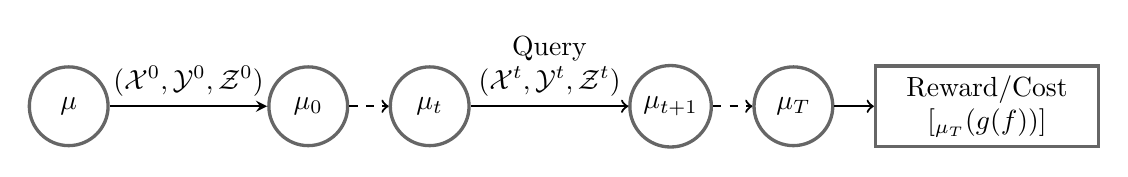
\begin{tikzpicture}
[
roundnode/.style={circle, draw=black!60, very thick, minimum size=10mm},
squarednode/.style={rectangle, draw=black!60, very thick, minimum size=10mm, align =center,text width = 26mm},
]
%Nodes
\node[roundnode]      (maintopic)                              {$\mu$};
\node[roundnode]        (circle1)       [right=20mm of maintopic] {$\mu_0$};
\node[roundnode]      (circle2)       [right=5mm of circle1] {$\mu_t$};
\node[roundnode]        (circle3)       [right=20mm of circle2] {$\mu_{t+1}$};
\node[roundnode]        (circle4)       [right=5mm of circle3] {$\mu_T$};
\node[squarednode]        (circle5)       [right=5mm of circle4] {Reward/Cost $\E \left[ \V_{\mu_T} (g(f))\right]$};


%Lines
\draw[thick, ->, >=stealth] (maintopic.east) -- node[anchor=south] {$(\mathcal{X}^0,\mathcal{Y}^0,\mathcal{Z}^0)$} (circle1.west);
\draw[thick, ->, dashed] (circle1.east) --  (circle2.west);
\draw[thick, ->] (circle2.east)  -- node[above, align =center, text width = 18mm] { Query $(\mathcal{X}^t,\mathcal{Y}^t,\mathcal{Z}^t)$} (circle3.west);
\draw[thick, ->,dashed] (circle3.east) --  (circle4.west);
\draw[thick, ->] (circle4.east) --  (circle5.west);


\end{tikzpicture}
\caption{MDP framework for adaptive labeling to efficiently estimate the average treatment effect (ATE).}
\label{fig:MDP_framework_flowchart}
\end{figure}
 









\begin{comment}
\subsection{Broader applicability of the framework to other problem settings} \label{sec:broad-framework-accuracy}
 

Although  we describe our setting in a healthcare setting with the objective  to estimate the recall of a trained AI model $\model(\cdot)$, the framework caters to many other problem settings. The extension to the evaluation of model based on accuracy (in regression setting) is straightforward, we simply replace the definition of recall $g(f)$ in~\eqref{eqn:l2-g-f} with
\begin{align*}
    g(f) = \E_{\substack{ y \sim p(y|f,x) \\  \forall x \in \mathcal X}} \big( \E_{{\textbf x} \sim p_x} [y-\model(x)]^2 \big).
\end{align*}


\textcolor{red}{To discuss if we need to have it here}
We can also extend this setting to the efficient estimation of the ATE as well. We describe these in detail below:

\begin{itemize}
    
    \item Estimating accuracy:  \[g(f) = \E_{\substack{ y \sim p(y|f,x) \\  \forall x \in \mathcal X}} \big( \E_{{\textbf x} \sim p_x} [y-\model(x)]^2 \big)\]
%    \item Estimating ATE with known control arm: 
%\[g(f) = \E_{\substack{ y \sim p(y|f,x) \\  \forall x \in \mathcal X}} \big( \E_{{\textbf x} \sim p_x} [y-\model(x)] \big)\]
\item Estimating ATE  (with minor modifications - broad structure remains similar) : 


Consider feature vector ${\mathbf x} \in \mathcal X $  distributed as ${\mathbf x}  \sim p_{\mathbf x}$, treatment $z \in {\mathcal Z} = \{0,1\}$, and a class of random functions $f: {\mathcal X} \times {\mathcal Z} \to {\mathcal Y}$, which determines the likelihood $p(y_i|f,{\mathbf x_i},z_i)$. Note that $f$ is random and reflects our uncertainty about how
labels are generated given features and the treatment. Additionally, the joint likelihood is determined as follows,  

\[p(Y|f,X,Z) = \prod_{i} p(y_i|f,{\mathbf x_i}, z_i) \]

Assuming the prior over functions $f$ to be $\mu$, therefore we have 
\[p(Y|X,Z) = \int \prod_{i} p(y_i|f,{\mathbf x_i},z_i) d\mu(f) \]


Also, assuming that under the  true data generating function $f$ (if known precisely - which we don't), the estimand of interest is

\[ \E_{{\textbf x} \sim p_x}  \left( \E_{\substack{ y \sim p(y|x,f,z=1) }} y - \E_{\substack{ y \sim p(y|x,f,z=0) }} y \right) \]


Throughout the paper we assume the above data generating process.  Now, suppose we have some labeled  data $(\datax^0,\datay^0,Z^0) =({\mathbf x}_{1:m}^0,y_{1:m}^0, z_{1:m}^0)$. 
    We run a experiment, in which we want to query the labels (in batches), so as to minimize the uncertainty of the estimand of interest. Suppose, the horizon of the experiment is $T$. Now, given prior $\mu$ and labeled data $\datax^0,\datay^0,Z^0$, in the beginning of our experiment the posterior state is $\mu_0$.

 At each step $j$ ($j \geq 1$), we query labels for a batch (with size $k$) of unlabeled data $(\datax^j,Z^j) \subset \mathcal X \times \mathcal Z$  and get labels $\datay^j$. After acquiring the labels at each step $j$ we update posterior state to $\mu_{j+1}$, informed by $\mu_j$ and $(\datax^j,\datay^j,Z^j)$. 
 
 Let the policy at step $j$ be $\pi_j$ (potentially random), which gives $\datax^{j+1},Z^{j+1} \sim \pi_j(\mu_j)$.  Observe that $\mu_{j+1}$ is random because of the randomness of the policy $\pi_j$ and $\datay^{j+1}|\{\datax^{j+1},Z^{j+1},\mu_j\}$ (\textcolor{red}{can this be written in a better way?}). Let, $\pi = \{\pi_0,....,\pi_{T-1}\}$. Therefore, our objective is to

 
\[ \min_{\pi} \E \left[ {\mathbf {Var}}_{f \sim \mu_T} \left( \E_{{\textbf x} \sim p_x}  \left( \E_{\substack{ y \sim p(y|x,f,z=1) }} y - \E_{\substack{ y \sim p(y|x,f,z=0) }} y \right) \right) \right]\]

where, $\mu_T$ depends on $\{(\datax^i,\datay^i,Z^i)\}_{i=0}^T$ and outer expectation is over both $\pi$ and  $\datay^{j+1}|\{\datax^{j+1}, Z^{j+1},\mu_j\}$ for all $j \in [0,T-1]$.


%Constraining the action space is straightforward - by first choosing set of x's using k-subset and then assigning treatment with learnable probability parameters $w_1,...,w_n$.

\end{itemize}

 \[ g(f) = \E_{\substack{ y \sim p(y|f,x) \\  \forall x \in \mathcal X}}\E_{{\textbf x} \sim p_x} g(y,{\textbf x}) \approx \E_{\substack{ y \sim p(y|f,x) \\  \forall x \in  \datax^u}} \left( \frac{1}{n}\sum_{i=1}^n \tilde{g}(y,{\textbf x}_i^u) \right)\]




Notation borrowed from a combination of the following papers 
~\citep{LeeYuNaFoLe23, KatoOgKoIn24, FongHoWa24}

%  
\end{comment}


%%% Local Variables:
%%% mode: latex
%%% TeX-master: "main"
%%% End:
     

\section{\label{sec:method}Methodology}

Each SIEM system uses its own RDL to define threat detection rules, and each RDL has its own schema.
For example, the Splunk SIEM uses the SPL to define its threat detection rules.
The task of understanding threat detection rules and recommending relevant MITRE ATT\&CK techniques (or sub-techniques) requires complex reasoning skills.
In the case of LLMs, this can be achieved with a technique called prompt chaining in which each task is divided into multiple sub-tasks in order to understand the complex reasoning behind the task.
Therefore, we employ a multi-phase architecture based on prompt chaining that leverages the power of LLMs to take a SIEM rule defined in any RDL and map it to relevant MITRE ATT\&CK techniques using the power of LLMs.
Our approach is based on the following intuitions:
\begin{itemize}[nosep,leftmargin=*]
    \item \textit{LLMs' implicit knowledge}: LLMs possess deep understanding of diverse RDLs. This enables them to interpret any rule, regardless of the RDL it is defined in, and convert it into comprehensible natural language text.
    \item \textit{LLMs' similarity comparison capability}: LLMs are adept at analyzing and comparing textual descriptions. 
    They can intelligently assess the similarity between two textual inputs to establish a meaningful connection.
\end{itemize}

\methodName has two main phases: (1) the rule to text translation phase, and (2) the MITRE ATT\&CK techniques recommendation phase.
These two phases in the pipeline include six key steps to determine relevant TTPs, as illustrated in Figure~\ref{fig:r2t}.

Although LLMs excel at translating SIEM rules into natural language, they often lack critical domain-specific contextual information related to IoCs in the rules.
To overcome this limitation, the \textit{rule to text translation} phase includes three steps: IoC extraction, contextual information retrieval, and natural language translation.

The workflow begins with the extraction of IoCs from the rules (for example, processes, log source, event codes, and file names) that the rule searches for in the logs (step (1)).In the next sstep a web search agent performs the task of obtaining additional contextual information about the IoCs discovered ((step 2)).
By incorporating this additional domain-specific information, the pipeline enhances the language translation, resulting in a more accurate and meaningful interpretation of SIEM rules.
The rule itself and the IoCs' contextual additional information from the previous stage are then used to translate the rule from RDL to natural language (step (3)).

The \textit{MITRE ATT\&CK techniques} recommendation phase of the pipeline includes the following three steps.
The rule in processed in data source identification step in which the probable origin of the data is identified (step (4)).
The description of the rule is then used to determine probable MITRE ATT\&CK techniques based on the implicit knowledge of the LLM (step (5)).
Finally, using chain-of-thought~\cite{wei2022chain} prompting, the most relevant techniques are extracted from the list of probable techniques (step (6)).
Each step of our method is further described in detail below.


% [bb=0 0 1440 900,width=1.43\linewidth,height=0.9\textwidth]
\begin{figure*}[htbp]
   \includegraphics[width=\textwidth]{Images/stages.jpg}
    
   \caption{An illustration of the different steps in \methodName.}
   \label{fig:stages}
\end{figure*} 

\subsection{IoC Extraction}
The context associated with a SIEM detection rule is crucial for its accurate interpretation and effective application. 
Obtaining this contextual understanding requires comprehensive analysis of the embedded IoCs in the SIEM rule.
In the first step, \methodName systematically identifies and extracts all IoCs, identifying the types of IoCs and their corresponding values that form the foundational elements of the detection rules. 
Leveraging the LLM's inherent understanding of rule structures and IoCs, we employ a zero-shot prompting approach for this task. 
Zero-shot prompting enables the direct extraction of IoCs from the rules without requiring extensive pre-training on specific datasets.

\noindent The result of this stage is a dictionary structure, where:
\begin{itemize}[nosep,leftmargin=*]
    \item Keys represent types of IoC, such as processes, files, IP addresses, and log sources.
    \item Values are lists containing specific IoC details, such as process names, file names, IP addresses, and log source identifiers.
\end{itemize}

In the example depicted in Figure~\ref{fig:stages}(a), the pipeline processes a rule for which relevant MITRE ATT\&CK techniques need to be recommended. 
The IoC extractor LLM produces a dictionary structure as output, organizing the IoCs in a structured format to support subsequent stages in the analysis pipeline. 



\subsection{Contextual Information Retrieval}
In this step, an LLM agent is employed to retrieve relevant information pertaining to the IoCs extracted from the rule.
A REACT agent~\cite{react} was used in this case to generate both reasoning traces and task-specific actions in an interleaved manner.
REACT agents interact with external tools to retrieve additional information that leads to more factual and reliable responses.
The LLM agent conducts a systematic search across web resources to gather additional contextual information for each IoC value present in the rule. 
This step addresses LLMS' lack of up-to-date knowledge or specialized domain expertise (which is critical to understanding the role and significance of the IoCs in the rule), without the need for retraining or fine-tuning.
Figure~\ref{fig:stages}(b) presents an example in which the rule includes the process name \texttt{soaphound.exe} as an IoC.
As can be seen, the web search results indicate that \texttt{soaphound.exe} is being used for active directory (AD) enumeration, which is important for the understanding of the attack. 

\subsection{Natural Language Translation}

The translation of detection rules into natural language textual descriptions fulfills three key objectives:
\begin{enumerate}[nosep,leftmargin=*]
    \item \textbf{Ensures that \methodName is format-agnostic}: It converts rules defined in various RDL formats into a generic, unstructured text format, ensuring compatibility with different SIEM systems, regardless of the specific rule format.
    \item \textbf{Provides contextual explanation}: It includes all relevant contextual information to produce a concise and comprehensible explanation of the rule.
    \item \textbf{Enhances the comprehension for LLMs}: It enables LLMs to more effectively compare the translated rule with descriptions in the MITRE ATT\&CK framework by providing a unified textual representation.
\end{enumerate}
To achieve these objectives, a zero-shot prompting technique is employed. 
The input to the LLM comprises two components:
\begin{itemize}
    \item \textbf{Syntactical information}: The rule itself, providing the structural and operational details.
    \item \textbf{Contextual information}: Details of the IoCs extracted from the rule, providing semantic insights into the rule's intent and function.
\end{itemize}
The LLM utilizes these inputs to generate a natural language textual description of the rule. 
This transformation not only ensures a more interpretable representation but also facilitates further steps of analysis and comparison, particularly in aligning the rule with MITRE ATT\&CK techniques and sub-techniques.



\subsection{Data Source or Mitigation Identification}
Identifying the most relevant data component or mitigation associated with the rule description in this step is critical for filtering out irrelevant MITRE ATT\&CK techniques (or sub-techniques) in subsequent steps of the pipeline.
In the MITRE ATT\&CK framework, data sources represent various categories of information that can be gathered from sensors or logs. 
These data sources include \textit{data components}, which are specific attributes or properties within a data source that are directly relevant to detecting a particular technique or sub-technique~. 
For example, in the context of the rule described in Figure~\ref{fig:stages}(a), the term \texttt{Endpoint.Processes} indicates that the activity is happening on an endpoint. 
Presence of the terms such as, \texttt{soaphound.exe}, \texttt{--buildcache}, \texttt{--certdump} and etc. indicate that the rule searches for command line execution of an executable named \texttt{soaphound.exe} with specific parameters. 
Therefore, the appropriate data source in this example is \textit{Command}, with the corresponding data component being \textit{Command Execution}.
Additionally, \textit{mitigations} are defined as categories of technologies or strategies that can prevent or reduce the impact of specific techniques or sub-techniques. 
The MITRE ATT\&CK framework explicitly establishes relationships between data components, mitigations, and techniques (or sub-techniques), enabling a systematic approach for identifying relevant elements.

To identify the most relevant data component or mitigation associated with a given rule description, we utilize agentic retrieval augmented generation (RAG), which incorporates an AI Agent-based implementation of the RAG framework.
Data from the MITRE ATT\&CK framework, specifically related to data components and mitigations, is stored in a vector database (e.g., ChromaDB). 
The process begins with the rule description from the previous stage, which serves as the input to the AI Agent. 
The LLM-powered agent automatically generates a search query tailored to retrieve relevant information from the RAG database.

For each query, the system retrieves the five most similar documents from the database, each containing contextual information about data components or mitigations. 
These documents are then utilized by the LLM agent to contextualize the rule description. 
By comparing the content of these retrieved documents with the rule description, the LLM agent determines and outputs the most relevant data component or mitigation along with a chain-of-thought as to why the data component or mitigation is related to the rule.


\subsection{Probable Technique Recommendation}

In this step, an LM agent is utilized to propose probable MITRE ATT\&CK techniques (and sub-techniques) that may be relevant to the description of the provided rule.
We used a REACT agent in this step as well to utilize both implicit and explicit knowledge during reasoning.
For explicit knowledge, the agent searches the MITRE ATT\&CK framework to obtain the list of probable techniques (and sub-techniques).
The natural language description of the rule from the previous step serves as input to the LLM agent.
The output of this stage consists of a list of JSON objects, each containing the MITRE technique ID, technique name, and technique description as seen in Figure~\ref{fig:stages}(c).

Throughout our experiments, we observed that as the number of recommendations ($k$) increases, both the framework's average recall and precision initially improve, however beyond a certain threshold of $k$, the %average 
precision begins to decline.
Based on these observations(please refer Table~\ref{tab:results3}), we selected a $k$-value of 11 to ensure a high recall.



\subsection{Relevant Technique Extraction}
In this step, \methodName refines the set of probable MITRE ATT\&CK techniques identified in the previous stage by eliminating irrelevant entries.
This step in the pipeline serves two primary purposes: (1) to enhance precision while maintaining recall achieved in previous step, and (2) to provide a clear rationale for the selection of the labels, ensuring transparency and interpretability of the mapping process.
This refinement process is grounded in the assumption that LLMs are effective for text similarity matching tasks.

The process comprises two key steps:
\begin{itemize}
    \item \textit{Rule-technique comparison}: The description of each technique in the set of probable techniques is compared with the rule description. 
    A chain-of-thought technique is then applied to elucidate the reasoning behind the association of each technique with the rule.
    \item \textit{Confidence calculation}: The generated chain-of-thought rationale for each technique (or sub-technique) is compared with the rule description to compute a relevance (or confidence) score, as done in prior work~\cite{freitas2024ai}.
    % \item \textbf{Reasoning}: \new{Add here the reasoning that it provides - explaining in NLP why it was selected...}
\end{itemize}

Techniques with higher confidence scores are deemed more relevant to the rule. 
Conversely, techniques with scores falling below a predefined threshold are excluded.
The techniques retained after this filtering step represent the most relevant techniques corresponding to the given rule's description. 


The chain-of-thought (CoT) rationale generated during the comparison of each rule to its probable technique is also provided as an output in this step.
This rationale offers a detailed natural language explanation, articulating why a particular technique is relevant to the given rule. 
Such explanations are highly valuable for security analysts, as they provide clear and transparent reasoning behind the mapping, enabling analysts to better understand and validate the association between the rule and the technique.
Other classification models proposed in previous works within this domain also suffer from the limitation of being black-box models, which lack the ability to provide clear reasoning or explanations. 
Unlike \methodName, these models fail to generate transparent, CoT rationales that explain why a particular rule is mapped to a specific technique, making them less interpretable and less useful for security analysts.    
\section{Experiments: Planning outperforms Heuristics}
\label{sec:experiment}

We begin our empirical demonstrations by showcasing the effectiveness of our planning framework on both synthetic and real datasets. We focus on the simplest planning algorithm, 1-step lookaheads (Algorithm~\ref{alg:complete}), and show that even basic planning can hold great promise. 
We illustrate our framework using two uncertainty quantification modules---GPs and 
\ensembles/ \ensembleplus. 

Throughout this section, we focus on evaluating the mean squared error of 
a regression model $\model$,  and develop adaptive policies that minimize uncertainty on $g(f)$ defined in~\eqref{eqn:l2-g-f}.
When GPs provide a valid model of uncertainty, 
our experiments show that our planning framework significantly outperforms other baselines. 
We further demonstrate that our conceptual framework extends to deep learning-based uncertainty quantification methods such as  \ensembleplus while highlighting computational challenges that need to be resolved in order to scale our ideas. 
For simplicity, we assume a naive predictor, i.e., $\psi(\cdot) \equiv 0$. However, we emphasize that this problem is just as complex as if we were using a sophisticated model $\psi(.)$. The performance gap between the algorithms 
primarily depends
on the level  of uncertainty in our prior beliefs.

To evaluate the performance of our algorithm, we benchmark it against several baselines. 
%Active learning baselines use an acquisition function $\ac$ to select points that have the highest   function value: $X\opt_t \in \argmax_{X \in \xpoolj{t}} \ac({X})$ at every step $t$. These methods may also need an UQ module, which we simply use the same UQ module as in our algorithm, and it  outputs $V(X)$ that measures the the uncertainty of each point $X \in \xpoolj{t}$.
Our first set of baselines are from active learning~\citep{AggarwalKoGuHaPh14}:
\\ % \noindent\textbf{Active Learning Heuristics:} 
\textbf{(1)} 
\textsf{Uncertainty Sampling (Static):}  In this approach, we query the samples for which the model is least certain about. Specifically, we estimate the variance of the latent output $f(X)$ for each $X \in \xpool$ using the UQ module and select the top-$K$ points with the highest uncertainty. \\
\textbf{(2)} \textsf{Uncertainty Sampling (Sequential):} This is a greedy heuristic that sequentially selects the points with the highest uncertainty within a batch, while updating the posterior beliefs using pseudo labels from the current posterior state. Unlike \textsf{Uncertainty Sampling (Static)}, this method takes into account the information gained from each point within batch, and hence tries to diversify the selected points within a batch. 

 
We also compare our approach to the  \textbf{(3)} \textsf{Random Sampling}, which selects each batch uniformly at random from the pool. Additionally, we compare solving the planning problem using  \textsf{REINFORCE}-based policy gradients with   $\mathsf{Smoothed\text{-}Autodiff}$ policy gradients.\footnote{Our code repository is available at
  \url{https://github.com/namkoong-lab/adaptive-labeling}.}
%Detailed experimental setups are provided in Section \ref{sec:details-experiments}.

%We repeat all experiments with 10 random seeds.




\begin{figure}[t]
\centering
\begin{minipage}[b]{0.49\textwidth}
\centering
\includegraphics[width=\textwidth, height=5cm]{figures/original_scale/Var_of_l_2_loss.pdf}
\caption{(Synthetic data) Variance of mean squared loss evaluated through the posterior belief $\mu_t$ at each horizon $t$. This is the objective that policy gradient methods like \textsf{REINFORCE} and $\ouralgo$ optimizes. 1-step lookaheads are surprisingly effective even in long horizons.}
\label{fig:var-l2-sim}
\end{minipage}
\hfill
\begin{minipage}[b]{0.49\textwidth}
\centering \includegraphics[width=\textwidth, height=5cm]{figures/original_scale/Error_of_estimated_model_l_2_loss.pdf}
\caption{(Synthetic data) Error between MSE calculated based on collected data $\mc{D}^{0:T}$ vs. population oracle MSE over $\mc{D}_{\rm eval} \sim P_X$. Reducing uncertainty over posteriors directly leads to better OOD evaluations. 1-step lookaheads significantly outperform active learning heuristics in small horizons.}
\label{fig:mean-l2-sim}
\end{minipage}
%\caption{Simulated data for GPs}
%\label{fig:both_plots}
\end{figure}

\subsection{Planning with Gaussian processes}
\label{sec:experiment-plan-GP}
We now briefly describe the data generation process for the GP experiments,  deferring a more detailed discussion of the dataset generation to Section~\ref{sec:details-experiments}. 
We use both the synthetic data and the real data to test our methodology.
For the \emph{simulated data},  we construct a setting where the general population is distributed across \emph{51 non-overlapping clusters} while the initial labeled data $\dtrain$ just comes from one cluster. In contrast, both $\dpool \defeq (\xpool,\ypool),\deval \defeq (\xeval,\yeval)$ are generated   from all the clusters. 
We begin with a low-dimensional scenario, generating a one-dimensional regression setting using a GP. %Gaussian Process (GP).
Although the data-generating process is not known to the algorithms,  we assume that the GP hyperparameters are known to all the algorithms
to ensure fair comparisons. This can be viewed as a setting where our prior is well-specified, allowing us to isolate the effects
of different policy optimization approaches
 without any concerns about the misspecified priors. We select $10$ batches, each of size $K=5$ across $T = 10$ time horizons.

To examine the robustness of our method against the distributional assumptions made  in the simulated case, we then move to a real dataset where the correct prior is not known. We simulate selection bias from the eICU dataset~\citep{PollardJoRaCeMaBa18}, which contains real-world patient data with in-hospital mortality outcomes. 
We conduct a $k$-means clustering to generate 51 clusters and then select data from those clusters. We view this to be a credible replication of practice, as severe distribution shifts are common due to selection bias in clinical labels.  To convert the binary mortality labels into a regression setting, we train a  random forest classifier and fit a GP on predicted scores, which serves as the UQ module for all the algorithms. As before, the task is to select 10 batches, each consisting of 5 samples, across 10 time horizons.

 In Figures~\ref{fig:var-l2-sim} and~\ref{fig:mean-l2-sim}, we present results for the simulated data. 
Figure~\ref{fig:var-l2-sim} shows the variance of $\ell_2$ loss, and Figure~\ref{fig:mean-l2-sim} presents the error in the estimated $\ell_2$ loss using $\mu_t$ (relative to true $\ell_2$ loss, that is unknown to the algorithm). 
As we can see from these plots, our method one-step lookahead  gives substantial improvements  over active learning baselines and random sampling. In addition,
compared to the one-step lookahead planning approach using \textsf{REINFORCE}-based policy gradients, 
we observe that $\mathsf{Smoothed\text{-}Autodiff}$-based policy gradients provide significantly more robust performance over all horizons.

In Figures~\ref{fig:var-l2-real}~and~\ref{fig:mean-l2-real}, we observe similar findings on the eICU data. We see that planning policies (\textsf{REINFORCE} and $\mathsf{Smoothed\text{-}Autodiff}$) consistently outperform other heuristics by a large margin.  Active learning baselines perform poorly in these small-horizon batched problems and can sometimes be even worse than the random search baselines.  Overall, our results show the importance of careful planning in adaptive labeling for reliable model evaluation. 

We offer some intuition as to why one-step lookahead planning may outperform other heuristic algorithms. 
 First,  \textsf{Uncertainty sampling (Static)} while myopically selects the
 top-$K$ inputs with the highest uncertainty, it fails to consider 
the overlap in information content among the ``best” instances; see \citep{AggarwalKoGuHaPh14} for more details. 
In other words,  it might acquire points from the same region with high uncertainty while failing to induce diversity among the batch.
Although \textsf{Uncertainty Sampling (Sequential)} somewhat addresses the issue of information overlap, a significant drawback of 
this algorithm
is the disconnect between the objective we aim to optimize and the algorithm. For example, it might sample from a region with high uncertainty but very low density. 

\begin{figure}[t]
\centering
\begin{minipage}[b]{0.48\textwidth}
\centering
\includegraphics[width=\textwidth, height=5cm]{figures/original_scale/Var_of_l_2_loss_real.pdf}
\caption{(Real-world eICU data) Variance of mean squared loss evaluated through the posterior belief $\mu_t$ at each horizon $t$. Even 1-step lookaheads are extremely effective planners, and auto-differentiation-based pathwise policy gradients provide a reliable optimization algorithm based on low-variance gradient estimates.}
\label{fig:var-l2-real}
\end{minipage}
\hfill
\begin{minipage}[b]{0.48\textwidth}
\centering \includegraphics[width=\textwidth, height=5cm]{figures/original_scale/Error_of_estimated_model_l_2_loss_real.pdf}
\caption{(Real-world eICU data) Error between MSE calculated based on collected data $\mc{D}^{0:T}$ vs. population oracle MSE over $\mc{D}_{\rm eval} \sim P_X$. Reducing uncertainty over posteriors directly leads to better OOD evaluations. Our method significantly outperforms active learning-based heuristics, and random sampling.}
\label{fig:mean-l2-real}
\end{minipage}
%\caption{Real data for GPs}
\end{figure}
 
%\vspace{-1.5cm}
% \begin{wrapfigure}{r}{.32\columnwidth}
%   \vspace{-.5cm} 
%   \centering
% \includegraphics[scale=.29]{figures/Var of l2l_2 loss.pdf}
%   \vspace{-0.2cm}
%   \caption{Results of GP}
% \label{fig:var-l2-gp}
%   \vspace{-0.1cm}
% \end{wrapfigure}


% Attempts have been made  in the past to address these  drawbacks heuristically  (see \citep{AggarwalKoGuHaPh14}). We give a unified computational framework while approaching the problem in a more principled manner and solving it more optimally.




\subsection{Planning with  neural network-based uncertainty quantification methods ($\ensembleplus$)}


We now provide a proof-of-concept that shows the generalizability of our conceptual framework  to the deep learning-based UQ modules, specifically focusing on $\ensembleplus$ due to their previously observed superior performance~\citep{OsbandWenAsDwIbLuRo23}. Recall that implementing our framework with deep learning-based UQ modules  requires us to retrain the model across multiple possible random actions $\bm{a}(\theta)$ sampled from the current policy $\pi_\theta$.
This requires significant computational resources, in sharp contrast to the GPs where the posteriors are in closed form and can be readily updated and differentiated. 

Due to the computational constraints, we test $\ensembleplus$ on a toy setting to demonstrate the generalizability of our framework. We consider a setting where the general population consists of four clusters, while the initial labeled data only comes from one cluster. Again we generate data using GPs.  The task is to select a batch of 2 points in one horizon. We detail the $\ensembleplus$ architecture in Section \ref{sec:details-experiments}, and we assume prior uncertainty to be large (depends on the scaling of the prior generating functions). 
The results are summarized in the Table~\ref{tab:UQ_ensemble}.

% \begin{table}[H]
% \vspace{-10pt}
% \caption{Performance under \ensembleplus as UQ module}
%     \centering
%     \begin{tabular}{|m{3cm}|m{2.5cm}|m{2cm}|} 
%     \hline
%       Algorithm   & Variance of $\loss_2$ loss estimate & Error of $\loss_2$ loss estimate  \\ \hline Random Sampling 
%          & $1710.9 \pm 1352.1$ & $8.67\pm6.62$ 
%       \\ \hline \ouralgo & $1.30 \pm 0.68$ & $0.91\pm0.25$ \\ \hline
%     \end{tabular}
%     \label{tab:UQ_ensemble}
%     %\vspace{-10pt}
% \end{table}




\begin{table}[h]
\vspace{-10pt}
\caption{Performance under \ensembleplus as the UQ module}
\centering
\begin{tabular}{|l|l|l|}
\hline
Algorithm   & Variance of $\loss_2$ loss estimate & Error of $\loss_2$ loss estimate  \\
\hline
\textsf{Random sampling} & 7129.8 $\pm$ 1027.0 & 136.2 $\pm$ 8.28 \\ \hline
\textsf{Uncertainty sampling (Static)} & 10852 $\pm$ 0.0 & 162.156 $\pm$ 0.0 \\ \hline
\textsf{Uncertainty sampling (Sequential)} & 8585.5 $\pm$ 898.9 & 144 $\pm$ 6.93 \\ \hline
\textsf{REINFORCE} & 1697.1 $\pm$ 0.0 & 45.27 $\pm$ 0.0 \\ \hline
\ouralgo & 1697.1 $\pm$ 0.0 & 45.27 $\pm$ 0.0 \\ \hline
\end{tabular}
%\caption{Comparison of different algorithms based on variance   and   error in $\ell_2$ loss estimation with Ensemble $+$ as the UQ module. Our results demonstrate that {\ouralgo} and REINFORCE outperformthe other active learning based heuristics, confirming the benefits of our MDP formulation for the adaptive labeling problem, as also demonstrated in Section 4.\\
%\footnotesize{Experimental details: We use Gaussian Processes as our data generating process, GP parameters are the same as in Section D.3.  The task is to select a batch of 2 points along one horizon.The marginal distribution $p_X$ has 4 \textit{non-overlapping} clusters. Initial data comes from one cluster, while pool and evaluation points comes from all the clusters. We have $20$ initial labeled data points, $10$ pool points, and $252$ evaluation points.  Training procedures are similar to the one in Section D.3.} }
\label{tab:UQ_ensemble}
\end{table}



% We faced  issues in scaling up these experiments which will be our focus in the future. 





% \begin{itemize}
%     \item Posteriors should be consistent. Two dimensions: even with less training,  
%     \item the inference should be  fast enough
% \end{itemize}


% Potential research directions for uncertainty quantification

% In this section we consider a simple setting We consider a simpler setting and 


% For synthetic dataset generation, we use ...... For real datasets, we use ...... We compare our methodolgy to several baselines ()    This Section is structured as follows:
% \begin{itemize}
%     \item \textbf{GPs, square loss objective} (Section \ref{}): 
%     %the broad aim of the experiments  in this section is to isolate the performance of our methodology without any concerns for the inefficiencies induced due to a mis-specified prior or imperfect posterior inference. To accomplish this we generate synthetic datasets using GPs (detailed later). We use the well specified prior (GPs - with same hyperparameter setting) as our UQ module.   
%      As GPs provide differentaible posterior inference - any errors induced due to imperfect posterior updates are also isolated. We note that under this setting
%      \item In Section\ref{} we demonstrate why our methodology performs better than other baselines - by devising various synthetic experiments ()
%     \item  \textbf{UQ Benchmarking }(Section \ref{}): Before diving into the experiments using $\ensembleplus$ and ENNs,  we showcase our benchmarking experiments in Section \ref{}. We use real datasets We observe that ENNs perform better
%      \item \textbf{Ensemble $+$}, objective: recall, accuracy
%     \item \textbf{ENN}, objective: recall, accuracy
% \end{itemize}




% In Section {}, we test 
% \subsection{Experimental details}

% \begin{itemize}
%     \item UQ methodologies - GPs, ENNs
%     \item Objectives - Recall,  ATE
%     \item Datasets - ATE-synthetic datasets, Recall-synthetic, real datasets
%     \item Baselines - 
%     \begin{itemize}
%         \item Random sampling
%         \item Active learning - Uncertainty based sampling - In regression setting almost all of the 
%         \item Myopic greedy - Greedy Batch based sampling
%         \item Policy Gradient
%     \end{itemize}
    
% \end{itemize}

% \subsection{Experiments}
%     \begin{itemize}
%     \item GPs with square loss
%     \item Benchmarking ENN
%         \item ENNs with ATE
%         \item ENNs with Recall
%     \end{itemize}

% \subsection{Benefits over other algorithms - intuition and experiments}

%Active learning - Myopic greedy / Don't rely on the objective rather some entropy version.


%%% Local Variables:
%%% mode: latex
%%% TeX-master: "main"
%%% End:


\newcommand{\cosim}{\mathsf{cosim}}


%Our codebase is available at \url{https://github.com/namkoong-lab/adaptive-labeling}.


\section{Analysis of Policy Gradient Estimators}
\label{sec:gradient_estimation_anlaysis}

In this section, we present a theoretical and empirical analysis of the statistical properties (bias-variance trade-off) of the \textsf{REINFORCE} and  $\mathsf{Smoothed\text{-}Autodiff}$ (smoothed-pathwise gradient) estimators and their efficacy
in downstream policy optimization task for adaptive labeling. First, in section \ref{sec:theory_gradient_estimation}, we theoretically compare the error in the $\mathsf{Smoothed\text{-}Autodiff}$ estimator and the \textsf{REINFORCE} estimator.
Next, in section \ref{sec:empirical_gradient_estimation_quality}, we empirically study the estimation quality of these two estimators within our framework, using  cosine similarity as the comparison metric. Finally, in section \ref{sec:gradient_estimation_algorithmic_performance}, we investigate the impact of gradient estimation quality on the performance of one-step lookaheads in the adaptive labeling setting.


%\textcolor{red}{Give a summary of the non-triviality of these results}.

%In this Section we present a theoretical and empirical analysis of when do smoothed pathwise gradients might out-perform \textsf{REINFORCE} gradients (and vice-versa) within our framework. Specifically, we present a bias-variance trade-off analysis for pathwise gradient and \textsf{REINFORCE} gradient -  

\subsection{Analytic insights}
\label{sec:theory_gradient_estimation}

 Recall that in our optimization problem (\ref{eqn:general-obj}), we encounter a combinatorial action space.
To build intuition, in Section~\ref{sec:theory_gradient_estimation_binary},   we start with a simple two-action setting to compare the 
$\mathsf{Smoothed\text{-}Autodiff}$ estimator and the \textsf{REINFORCE} estimator. 
The more  general setting is discussed in Section~\ref{sec:theory_gradient_estimation_multi}. 


 \subsubsection{Binary actions}
\label{sec:theory_gradient_estimation_binary}


To compare the two estimators, we consider a simplified setting with two possible actions 
$A \in \mathcal{A} := \{-1,1\}$, where the policy is parametrized by
$\theta \in [0,1]$, with
$\pi_\theta(-1) = \theta$ and $\pi_\theta(1) =1-\theta$. We are interested in the gradient $\nabla_\theta H(\theta)$, where $H(\theta) =\E_{A\sim \pi_\theta}G(A)$. For simplicity, we set $G(A)=A$.

\noindent Given $N$ i.i.d. samples of $A_i \sim \pi_\theta$, the \textsf{REINFORCE} estimator for $\nabla_\theta H(\theta)$ is defined as
\begin{align}
    \hat{\nabla}^{\mathsf{RF}}_N = \frac{1}{N}\sum_{i=1}^N\Big(G(A_i) \nabla_\theta \log(\pi_\theta(A_i)) \Big).
    \label{eqn:bin-reinf-def}
\end{align}
Using  the reparametrization trick, we can rewrite  $H(\theta)$ as $\E_U G(h(U,\theta))$, where 
\begin{align*}
    h(U,\theta):= 2\mc{I}(U > \theta)-1\stackrel{d}{=}A,
\end{align*}
with $U\sim \mathsf{Uni}[0,1]$. However, $h(U,\theta)$ is not differentiable with respect to $\theta$. Therefore, to enable the pathwise gradient estimation, we consider a smoothed approximation $ h_\tau(U,\theta)$ of $ h(U,\theta)$:
\begin{align*}
    h_{\tau}(U,\theta) = \frac{\exp\left(\frac{U-\theta}{\tau}\right)-1}{\exp\left(\frac{U-\theta}{\tau}\right)+1},
\end{align*}
where $\tau$ is a temperature parameter that controls the smoothness of $h_\tau(U,\theta)$.

\noindent The $\mathsf{Smoothed\text{-}Autodiff}$ estimator $\nabla_{\tau,N}^{\mathsf{grad}}$ is the $N$-sample approximation of 
$\E_{U}[\nabla_\theta G(h_{\tau}(U,\theta))]$, 
 given by
\begin{align}
    \hat{\nabla}^{\mathsf{grad}}_{\tau,N} = \frac{1}{N}\sum_{i=1}^N\Big(\nabla_\theta{G}(h_\tau(U_i,\theta))\Big).
    \label{eqn:bin-grad-def}
\end{align}
 Our result, with proof in Section~\ref{sec:proof-thm-binary},
 highlights the conditions under which 
 $\hat{\nabla}^{\mathsf{grad}}_{\tau,N}$~\eqref{eqn:bin-grad-def} achieves better gradient estimation (lower mean squared error)  compared to $\hat{\nabla}^{\mathsf{RF}}_{N}$~\eqref{eqn:bin-reinf-def}.
\begin{theorem}
For $\theta \in [0,1]$ and $N \le  \frac{1}{4\theta(1-\theta)} - 1$,
there exists $\Tilde{\tau}$ depending on $(N, \theta)$ such that 
\begin{align*}
\mse(\hat{\nabla}^{\mathsf{grad}}_{\Tilde{\tau},N})
< 
\mse(\hat{\nabla}^{\mathsf{RF}}_{N}).
\end{align*}
Additionally, for any $N$, $\theta = \frac{1}{k}$, and $k \to \infty$, we have that
$\mse(\hat{\nabla}^{\mathsf{RF}}_{N})  = \Omega(k) 
$, $\mse(\hat{\nabla}^{\mathsf{grad}}_{\tilde{\tau},N}) < 4$. 
The same statement holds for $\theta =  1-\frac{1}{k}$ as well. 
This implies that the MSE of $\hat{\nabla}^{\mathsf{RF}}_{N}$ is unbounded, while the MSE of gradient estimator is bounded.
\label{thm:binary}
\end{theorem}
\noindent In particular, this example illustrates how $\mathsf{Smoothed\text{-}Autodiff}$ gradients shine when 
the sample size $N$ is small and the policy takes on extreme values.

\subsubsection{General case}
\label{sec:theory_gradient_estimation_multi}

We now extend our analysis from Section~\ref{sec:theory_gradient_estimation_binary} to the setting with more than two actions.
Consider an  action space  $\mathcal{A}:= \{a_1,a_2,...,a_m\} \subset \mathbb{R}$ with $m \ge 2$ actions. 
Actions $A\in \mathcal{A}$ are drawn according to a policy $\pi_\theta$, such that $A=a_i$ with probability $\pi_\theta(a_i) = \frac{\theta_i}{\sum_{j=1}^m \theta_j}$. 
As in Section~\ref{sec:theory_gradient_estimation_binary}, we are interested in the gradient $\nabla_\theta H(\theta)$, where $H(\theta) =\E_{A\sim \pi_\theta}G(A)$. We assume that 
$G(\cdot)$ is differentiable and  sufficiently smooth such that
$G'(a) \le \bar{G}$ for all $a \in \mathsf{conv}(a_1,...,a_m)$. 
 %Assume that an action is sampled based on the policy $\pi_\theta$ as follows:
% \begin{align*}
%     \pi_\theta(a_i) = \frac{\theta_i}{\sum_{j=1}^m \theta_j}.
% \end{align*}

% \noindent To avoid complexities, below we consider a simple setting to convey intuition of why 
% our autodiff estimator performs better than the \textsf{REINFORCE} gradient estimator.

% \noindent \textbf{Specific Setting:} Let $\mathcal{A} = \{1,2,...,m\}$, with $\pi_\theta(i) = \frac{\theta_i}{\sum_{j=1}^m \theta_j}$. \textbf{Let $f(A) =A$.} 

% \vspace{5mm}


% \[\E_{A\sim \pi_\theta}(G(A)) = \sum_{i=1}^m \frac{\theta_i}{\sum_{j=1}^m \theta_j} G(a_i)\]


% \[\nabla_{\theta_i} \E_{A\sim \pi_\theta}(f(A)) =  
% \frac{
% f(a_i) (\sum_{j=1}^n \theta_j) - (\sum_{j=1}^n   \theta_j f(a_j))
% }{(\sum_{j=1}^n \theta_j)^2} \]

% \[\nabla_{\theta} \E_{A\sim \pi_\theta}(f(A)) =  
% \frac{
% 1}{ \sum_{j=1}^n \theta_j} \bm{f(a)} - \frac{\sum_{j=1}^n   \theta_j f(a_j)
% }{(\sum_{j=1}^n \theta_j)^2} \bm{1} \]


% Another helpful expression
% \[\nabla_{\theta_i} \E_{A\sim \pi_\theta}(f(A)) =  \frac{ \sum_{j=1}^n \theta_j (f(a_i)-f(a_j))}{(\sum_{j=1}^n \theta_j)^2} \]

% \paragraph{\textsf{REINFORCE} estimator} 
% $\nabla^{\mathsf{RF}}_{\theta_i} H(\theta) = \nabla_{\theta_i}  \E_{A\sim \pi_{\theta}} G(A) = {\E_{A\sim \pi_\theta} \Big(G(A) \nabla_{\theta_i} \log(\pi_\theta(A))} \Big)$



% To estimate it we take $N$ monte-carlo samples -

\noindent As in~\eqref{eqn:bin-reinf-def}, given $N$ i.i.d. samples of $A_j \sim \pi_\theta$,
the \textsf{REINFORCE} estimator 
is defined as
\begin{align}
\hat{\nabla}^{\mathsf{RF}}_{N,\theta_i}
\defeq 
\frac{1}{N}\sum_{j=1}^N\Big(G(A_j) \nabla_{\theta_i} \log(\pi_\theta(A_j)) \Big).
\label{eqn:eq-def-reinforce}
\end{align}

% Therefore, the expected squared error in the Reinforce estimator is  
% \[ \E[\\mse_i(\hat{\nabla}^{\mathsf{RF}}_{N,\theta_i})] = \frac{1}{N} \V_{A \sim \pi_\theta} \bigg(G(A) \nabla_{\theta_i} \log(\pi_\theta(A)) \bigg)\]


%\paragraph{Autodiff estimator (using gumbel softmax)} 

\noindent We now generalize the $\mathsf{Smoothed\text{-}Autodiff}$ estimator in ~\eqref{eqn:bin-grad-def}. Recall that $H(\theta) = \E_{A\sim \pi_\theta} {G}(A)$,  which can be rewritten as $$H(\theta) =  \E_{A\sim \pi_\theta}\left[ G \left(\sum_{i=1}^ma_i (\mc{I}(A)=a_i) \right) \right].$$
 Using the Gumbel-Max reparametrization trick  
 from~\citep{JangGuPo17}, we have
\begin{align*}
\{\mc{I}(A=a_i)\}_{i=1}^m 
\deq 
\tilde{h}(Z,\theta) \defeq
\mathsf{one\_hot}\left[ \argmax_i\set{\log(\theta_i) + Z_i} \right]
\end{align*}
 with  $Z_i$ being i.i.d samples drawn from Gumbel (0, 1), ensuring that 
  $A \sim \pi_\theta$. 
  
  
 \noindent Therefore, we can now express   $H(\theta) = \E_Z[G\left(h(Z,\theta) \right)]$, where $h(Z,\theta) = \tilde{h}(Z,\theta) \odot (a_i)_{i=1}^m $, the element-wise product  of $\tilde{h}(Z,\theta)$ and  the vector $(a_i)_{i=1}^m$. 
Since $h(Z,\theta)$ is not differentiable with respect to $\theta$, to enable pathwise gradient estimation, we consider a smoothed approximation $h_\tau(Z,\theta)$ of $ h(Z,\theta)$, as described in~\citep{JangGuPo17}:
\begin{align*}
h_\tau(Z,\theta)  
=
\left( \frac{\exp((\log (\theta_i)+Z_i)/\tau)}{\sum_{j=1}^{m}\exp((\log (\theta_j)+Z_j)/\tau)}\right)_{i=1}^m \odot (a_i)_{i=1}^m,
\end{align*} 
where $\tau$ is a temperature parameter controlling the smoothness of $h_\tau(Z,\theta)$. Thus, $$H(\theta)  \approx 
\frac{1}{N}\sum_{j=1}^N G(h_\tau(Z^{(j)},\theta)).$$
We now define the $\mathsf{Smoothed\text{-}Autodiff}$ estimator as
\begin{align}
  \hat{\nabla}^{\mathsf{grad}}_{\tau, N,\theta_i}
  \defeq \frac{1}{N}\sum_{j=1}^N\nabla_{\theta_i}G(h_\tau(Z^{(j)},\theta)).
\label{eqn:eq-def-autodiff}
\end{align}

We present our main result, Theorem~\ref{thm:multi}, for the $\mathsf{Smoothed\text{-}Autodiff}$ estimator defined in~\eqref{eqn:eq-def-autodiff} and \textsf{REINFORCE} estimator defined in~\eqref{eqn:eq-def-reinforce}.  Similar to Theorem~\ref{thm:binary},
the result below highlights 
that the \textsf{REINFORCE}  estimator will be worse
as compared to the $\mathsf{Smoothed\text{-}Autodiff}$ estimator
if the number of samples $N$ is not   large enough.
The proof is provided in Section~\ref{sec:proof-thm-multi}:
% but our results extend to the below estimator that we use in our pipeline:
%  \begin{align}
%   \Tilde{\nabla}^{\mathsf{grad}}_{N,\theta_i}
% \defeq  \nabla_{\theta_i}
%   G\left(  \sum_{i=1}^m a_i (h_\tau(Z,\theta))_i \right) \label{eqn:eq-def-autodiff-inside}
% \end{align}


% \begin{align}
%       \hat{\nabla}^{\mathsf{grad}}_{N,\theta_i}' =
%       f'\left(  \sum_{i=1}^m a_i (h_\tau(Z,\theta))_i \right)
%       \cdot 
%       \left( \sum_{i=1}^m a_i  \nabla(h_\tau(Z,\theta))_i \right)
% \end{align}

%  a∈[amina \in [a_{\min},a_{\max}],
% where a_{\min} = \min_{i=1}^m a_ia_{\min} = \min_{i=1}^m a_i


\begin{theorem}
Assuming
$G(\cdot)$ is differentiable and  sufficiently smooth such that
$|G'(a)| \le \bar{G}$ for all $a \in \mathsf{conv}(a_1,...,a_m)$. 
Fix $i \in [m]$.
For $\theta \in [0,1]^m$, any $\epsilon>0$ and 
\begin{align*}
N \le 
\frac{1}{\paran{\nabla_{\theta_i} \E_{A\sim \pi_\theta}(G(A))+\epsilon}^2}
\paran{
\frac{\sum_{j=1}^m\theta_j(G(a_j))^2}{(\sum_{j=1}^m\theta_j)^3} + \frac{(G(a_i))^2}{\theta_i\sum_{j=1}^m \theta_j} - 2 \frac{(G(a_i))^2}{(\sum_{j=1}^m \theta_j)^2}  - \left(\nabla_{\theta_i} \E_{A\sim \pi_\theta}(G(A))\right)^2},
\end{align*}
there exists $\Tilde{\tau}$ depending on $ (N, \theta)$ such that 
\begin{align*}
\mse(\hat{\nabla}^{\mathsf{grad}}_{\Tilde{\tau},N,\theta_i})
\le 
\left(\nabla_{\theta_i}\E_{A\sim \pi_\theta}(G(A))\right)^2 + {\epsilon}
\le 
\mse(\hat{\nabla}^{\mathsf{RF}}_{N,\theta_i}).
\end{align*}



 

Additionally, for any $N$, $\theta_i = \frac{1}{k}$, and $k \to \infty$, we have the following
\begin{align*}
\mse(\hat{\nabla}^{\mathsf{RF}}_{N,\theta_i}) & = \Omega(k),
 \mse(\hat{\nabla}^{\mathsf{grad}}_{\tilde{\tau},N,\theta_i})
 \le 
\left(\nabla_{\theta_i} \E_{A\sim \pi_\theta}(G(A))\right)^2.
\end{align*}

The same statement holds for $\theta_i =  1-\frac{1}{k}$ as well. This implies that the mse of $\hat{\nabla}^{\mathsf{RF}}_{N}$ is unbounded, while the mse of gradient estimator is bounded.
\label{thm:multi}
\end{theorem}





% If we assume 
% GG is sufficiently smooth: i.e., suppose
% G'(x) \le \bar{G}G'(x) \le \bar{G} for all xx, we can obtain the same results  while
% changing~\eqref{eqn:eq-def-autodiff}\eqref{eqn:eq-def-autodiff} to~\eqref{eqn:eq-def-autodiff-inside}\eqref{eqn:eq-def-autodiff-inside} carrying out similar analysis.




%In this Section, we demonstrate the bias-variance trade-off between the \textsf{REINFORCE} and pathwise gradient through its impact on the algorithmic performance and by also evaluating the mean-squared error and cosine similarity between the gradient estimators from each approach to the true gradient.


\subsection{Empirical comparison of gradient estimators}

\label{sec:empirical_gradient_estimation_quality}

In  the preceding theoretical analysis, we demonstrate  that $\mathsf{Smoothed\text{-}Autodiff}$ gradients can outperform \textsf{REINFORCE} gradients and there exists a temperature for which the mean squared error (MSE) of the $\mathsf{Smoothed\text{-}Autodiff}$ estimator is lower than that of the \textsf{REINFORCE} estimator.  While it is theoretically challenging to precisely characterize the difference between the $\mathsf{Smoothed\text{-}Autodiff}$ and \textsf{REINFORCE} gradients for varying $N$ and temperature $\tau$, we provide an empirical analysis of the gradient estimation within our adaptive labeling framework to further assess this comparison. 


As discussed, we denote the true gradient by $\nabla_{\theta}H(\theta)$.  For any gradient estimator $\hat{\nabla}_N $ (either $\hat{\nabla}_{\tau,N}^{\mathsf{grad}}$ or $\hat{\nabla}_N^{\mathsf{RF}}$), we measure the following performance metric, the cosine similarity, with the true gradient, denoted by $\cosim(\hat{\nabla}_N)$:
\begin{align*}
\cosim(\hat{\nabla}_N) = \E[\cos(\hat{\nabla}_N, \nabla_{\theta}H(\theta))],
\end{align*}
% \begin{align}
%     mse(\hat{\nabla}_N) = \frac{1}{d}\E[\mathbf{1}^T(\hat{\nabla}_N-\nabla_{\theta}H(\theta))^2]
% \end{align}
where expectation is taken over the randomness of the $\hat{\nabla}_N$.
Cosine similarity measures the alignment of direction between $\hat{\nabla}_N$ and $\nabla_{\theta}H(\theta)$, capturing both the bias and variance of the gradient estimators. 
The \textsf{REINFORCE} estimator is unbiased but suffers from high variance. As a result 
$\E [\cos(\hat{\nabla}_N^{\mathsf{RF}}, \nabla_{\theta}H(\theta))]$ might be small, even though $\E[\hat{\nabla}_N^{\mathsf{RF}}]= \nabla_{\theta} H(\theta)$.  
For the  $\mathsf{Smoothed\text{-}Autodiff}$  gradient, the $\cosim$ metric $\E [\cos(\hat{\nabla}_{N,\tau}^{\mathsf{grad}}, \nabla_{\theta}H(\theta))]$ is influenced by two factors. First, the  bias in the $\mathsf{Smoothed\text{-}Autodiff}$ gradient,  $\E (\hat{\nabla}_{N,\tau}^{\mathsf{grad}}) - \E (\nabla_{\theta}H(\theta))$, increases as $\tau$ increases. 
Second, the variance of the $\mathsf{Smoothed\text{-}Autodiff}$ gradient, $\V(\hat{\nabla}_{N,\tau}^{\mathsf{grad}})$,  decreases as $\tau$ increases. Our objective is to determine whether a favorable trade-off between bias and variance can be achieved, resulting in higher $cosim$ values and improved gradient alignment for the $\mathsf{Smoothed\text{-}Autodiff}$ gradient.













\begin{figure}
\centering
\begin{minipage}[b]{0.32\textwidth}
\centering
\includegraphics[height=4cm, width=5cm]
{figures/compare_grad_cos_tau_0.1.pdf}
\centering{\small{{$\tau=0.1$ }}}
\end{minipage}
\hfill
\begin{minipage}[b]{0.32\textwidth}
\centering
\includegraphics[height=4cm, width=5cm]{figures/compare_grad_cos_tau_0.5.pdf}
\centering{\small{ $\tau=0.5$}}
\end{minipage}
\hfill
\begin{minipage}[b]{0.32\textwidth}
\centering \includegraphics[height=4cm, width=5cm]{figures/compare_grad_cos_tau_10.pdf}
\centering{\small{$\tau=10$}}
\end{minipage}
\caption{Comparison of $\mathsf{Smoothed\text{-}Autodiff}$ and \textsf{REINFORCE} estimators under different temperature ($\tau$) hyperparameter for the $\mathsf{Smoothed\text{-}Autodiff}$ gradient - metric used is cosine similarity}
\label{fig:compare-grad-cos}
\end{figure}




 


In the below mentioned results, we compare the $\mathsf{Smoothed\text{-}Autodiff}$ gradients and  \textsf{REINFORCE} gradients in the setting discussed in 
Figures~\ref{fig:var-l2-sim} and~\ref{fig:mean-l2-sim}.  
To approximate the ground truth gradient $\nabla_{\theta}H(\theta)$, we use the unbiased \textsf{REINFORCE} gradient estimated over many samples (in our case, $10^6$ samples). We evaluate both  $\mathsf{Smoothed\text{-}Autodiff}$ and \textsf{REINFORCE} gradients for different values of $N$. 
To estimate the expected values of cosine similarity, each gradient estimator was computed $200$ times. Figure~\ref{fig:compare-grad-cos} compares the $\mathsf{Smoothed\text{-}Autodiff}$ estimator and the \textsf{REINFORCE} estimator for different $N$.
We observe that for different $N$, pathwise estimator outperforms the \textsf{REINFORCE} estimator and has higher cosine similarity.
Moreover, \textsf{REINFORCE} estimator takes almost 100-1000 times more samples to reach the same level of cosine similarity.

%https://github.com/namkoong-lab/adaptive_sampling/blob/main/src/notebooks/new_plots/Plot_1006.ipynb
%We present here the results for one $\theta$, and relegate results for other $\theta$'s and other settings to the Appendix.




 
%Similar results were observed for different settings and $\theta$'s (we refer the reader to the Appendix \ref{}). 
%One may wonder that why cosine smilarity is so low for the both estimators - this is because coisne similarity scales poorly with dimesnion of the vector, $\theta$ in our setting is of dimension $285$. When we take multiple gradient steps the grad's correct for itself - as far as cosine similarity is positive with high probability, however lower the cosine similarity, more the number of steps it takes to converge. In Fig \ref{}, we demonstrate that cosine similarity is comparatively higher in a setting where $\theta$ has low dimension $d=10$. 

%In Figure \ref{}, we demonstrate the bias-variance trade-off between the pathwise gradient estimator as we vary the temperature. we also observe a range of temperature where the  pathwise gradient estimator performs better than reinforce estimator.

%\textcolor{red}{@EVERYONE : Should we have the results for gradient estimators for different $\theta$ and settings in the Appendix and reference it here?}



\subsection{Impact of gradient estimation on algorithmic performance}
\label{sec:gradient_estimation_algorithmic_performance}

We now compare the performance of $\mathsf{Smoothed\text{-}Autodiff}$  and \textsf{REINFORCE} gradients in the downstream optimization task of adaptive labeling, examining the effect of varying the number of samples $N$ used in the gradient estimator. Our results show that gradient quality directly impacts downstream task performance. In Figures~\ref{fig:var-l2-sim-in-N} and~\ref{fig:mean-l2-sim-N}, we   replicate the setting from 
Figure~\ref{fig:var-l2-sim} and~\ref{fig:mean-l2-sim}  in Section~\ref{sec:experiment-plan-GP}. As illustrated, $\mathsf{Smoothed\text{-}Autodiff}$ gradients perform exceptionally well even with a single sample in the estimator, with only marginal gains as $N$ increases due to limited room of improvement. In contrast, \textsf{REINFORCE} performs poorly with one sample but gradually improves as the sample size increases.

 
%In Figure \ref{}, we show the bias-variance tradeoff in pathwise gradient as we vary the temperature $\tau$ manifesting in the performance on adaptive labeling task.




\begin{figure}[t]
\centering
\begin{minipage}[b]{0.49\textwidth}
\centering
\includegraphics[width=\textwidth, height=6cm]{figures/original_scale/N_samples_var_square_loss.pdf}
\caption{Comparing the impact of $\mathsf{Smoothed\text{-}Autodiff}$ and \textsf{REINFORCE} gradient estimators (with different values of $N$) on the performance of  \ouralgo. (Synthetic data) Variance of mean squared loss evaluated through the posterior belief $\mu_t$ at each horizon $t$.}
\label{fig:var-l2-sim-in-N}
\end{minipage}
\hfill
\begin{minipage}[b]{0.49\textwidth}
\centering \includegraphics[width=\textwidth, height=6cm]{figures/original_scale/N_samples_l2_loss.pdf}
\caption{Comparing the impact of $\mathsf{Smoothed\text{-}Autodiff}$ and \textsf{REINFORCE} gradient estimators (with different values of $N$) on the performance of  \ouralgo. (Synthetic data) Error between MSE calculated based on collected data $\mc{D}^{0:T}$ vs. population oracle MSE over $\mc{D}_{\rm eval} \sim P_X$.}
\label{fig:mean-l2-sim-N}
\end{minipage}
\end{figure}




\section{Practical considerations in implementing our framework}
\label{sec:practical_consideration}

As highlighted in our previous discussion, the success of our framework relies on  two critical components.  
First, the uncertainty quantification methodology must provide reliable and efficiently computable posterior updates. 
Second, the computational efficiency of the autodifferentiation software framework is crucial, 
as it enables end-to-end gradient estimation through the entire pipeline. 
This efficiency will be particularly important in multi-step lookahead scenarios. 
In this section, we highlight practical considerations associated with these two components, 
and discuss  remaining challenges and corresponding promising future research directions. 
We begin by evaluating the reliability of current UQ methodologies in Section~\ref{sec:eval_posterior_consis}, followed by a discussion on the efficiency of the autodiff framework in Section~\ref{sec:auto-diff-bottleneck}.


\subsection{Evaluating Posterior Consistency of Uncertainty Quantification Methods}
\label{sec:eval_posterior_consis}
The reliability of a UQ methodology depends on two key properties i) reliable UQ performance on out-of-distribution (OOD) inputs, and ii) the ability to sharpen beliefs reliably as more data is gathered. We refer to these two properties collectively as  ``posterior consistency''. 


% In this section, we evaluate and compare different UQ methodologies for their reliability (posterior consistency).  Given that Uncertainty Quantification is the foundational for fields such as trustworthy AI, active learning, and exploration in reinforcement learning - this analysis may be of independent interest to researchers in  these domains.  Most existing literature on UQ evaluation  focuses on static single-shot settings~\citep{OsbandWenAsDwIbLuRo23}, with some literature on evaluating UQ performance on OOD data~\citep{OvadiaFeReNa19,Nadoal21}. To our knowledge, none of these literature evaluates UQ in dynamic settings, which is critical for applications in active Learning and reinforcement learning settings. Continual learning~\citep{WangZhSuZh24} is an active area of research with a primary focus on efficiently retraining the models as new data is observed. In contrast, our focus on assessing whether a UQ model, even when retrained perfectly, performs posterior updates consistently—specifically, whether the posteriors are sharp on observed data and provide reliable UQ on unobserved data.

Most existing literature on UQ evaluation  focuses on static single-shot settings~\citep{OsbandWenAsDwIbLuRo23}, with some literature on evaluating UQ performance on OOD data~\citep{OvadiaFeReNa19,Nadoal21}. To our knowledge, none of these literature evaluates UQ in dynamic settings, which is critical for applications in active learning and reinforcement learning settings. 
In this section,  we focus on assessing whether a UQ model, 
even  
when retrained perfectly, performs posterior updates consistently or not—--specifically, whether the posteriors are sharp on observed data and provide reliable UQ on unobserved data. 
Since UQ is foundational to trustworthy AI and active exploration in reinforcement learning, our empirical insights may be of independent interest to researchers in these domains.  

Our experiments reveal several challenges that current UQ methodologies suffer from. Due to the variation in UQ quality across hyperparameters, we observe a clear trade-off between in-distribution (ID) and out-of-distribution (OOD) performance. 
The performance disparity between ID and OOD performance is intricately tied to canonical model training practices that extend beyond the conceptual UQ paradigms. In particular, we observe that implementation details such as weight-decay, prior scales (where applicable), and stopping times have an outsized influence on the performance of UQ methodologies. Moreover, we highlight
the unreliability of typical approximate posterior update heuristics,
which rely on gradient updates to the underlying network(s). 
We observe large variation in the quality of the posterior across similar implementation details and even random seeds,
underscoring the importance of further methodological development along these dimensions. 
These challenges magnify in the dynamic setting where posteriors are updated with new observations, highlighting the need for reliable posterior update methods---an often  overlooked dimension in UQ algorithmic development predominantly focused on static evaluations.  

We demonstrate the above discussion using the eICU dataset. Additional results from other datasets, along with further details on the evaluated UQ methodologies, the selection biases introduced, and the metrics used to assess UQ performance, are provided in
Section~\ref{sec:practical_consideration_experiment_details}.
 
\begin{figure}
\centering
\begin{minipage}[b]{0.32\textwidth}
\centering
\captionsetup{labelformat=empty,labelsep=none}
\includegraphics[height=4.5cm]
{figures/eicu_simple/Task_1_kl_estimate_dyadic_tau_10_ood_vs_k_val_for_all_agents.pdf}
{\small{\centering{eICU (Linear bias)}}}
\end{minipage}
\hfill
\begin{minipage}[b]{0.32\textwidth}
\centering
\includegraphics[height=4.6cm]{figures/eicu_clustering/Task_1_joint_log-loss_ood_vs._k_val_for_num_batches=200_dynamic_0.pdf}
{\small{ eICU (Clustering bias)}}
\end{minipage}
\hfill
\begin{minipage}[b]{0.32\textwidth}
\centering \includegraphics[height=4.5cm]{figures/GP_dynamic_0/Task_1_kl_estimate_dyadic_tau_10_ood_vs._k_val_for_num_batches=250_dynamic_0.pdf}
{\small{ Synthetic (Clustering bias)}}
\end{minipage}
\caption{Joint log-loss on OOD data with increasing selection bias. 
Though some agents such as ensemble and dropout perform well under no selection bias, their performance deteriorates significantly with a large selection bias (larger $k$).}
\label{fig:task-1-joint-ood-all-data}
\end{figure}



\paragraph{Performance under distribution shifts} In Figure~\ref{fig:task-1-joint-ood-all-data}, we compare the performance of different UQ methodologies on  out-of-distribution data under increasing levels of  \emph{linear} and \emph{out-of-support} selection bias. The methodology to introduce selection bias is detailed later in Section~\ref{sec:selection-bias}.
 Figure~\ref{fig:task-1-joint-ood-all-data} shows that most UQ methodologies are sensitive to selection bias, with performance often degrading  significantly on OOD data, while in-distribution performance remains stable.  These results emphasize the importance of evaluating UQ models beyond the data it has seen so far.



 
\paragraph{Hyperparameter tuning breaks under distribution shifts} 
UQ methodologies such as \ensembles/ \ensembleplus and Epinet require extensive hyperparameter tuning to perform well. Canonically, these hyperparameters are tuned by splitting the available dataset, $\mc{D}_0$, into a training and validation sets, and choosing the hyperparameters that yield the best results on the validation set.
However, we demonstrate that this approach has a significant limitation when the data experiences distribution shifts: the best hyperparameters for in-distribution (ID) data are not necessarily the best for out-of-distribution (OOD) test data. 
Moreover, in many cases, there is a unexpected trade-off between ID and OOD performance. In Figure~\ref{fig:difficult_to_choose_prior_scale}, we illustrate this phenomenon for  \ensembleplus, Epinets, and Hypermodels 
when tuning the Prior Scale hyperparameter (we provide a detailed explanation of each methodology in Section \ref{sec:UQ_bench_benchmark-uq-metric}). We observe that reducing prior scale for \ensembleplus improves ID  performance while the OOD performance deteriorates. Similar trends were noted for other hyperparameters, such as weight decay and stopping time, as shown in Figures~\ref{fig:difficult_to_choose_weight_decay} and~\ref{fig:difficult_to_choose_stopping_time} in Section \ref{sec:practical_consideration_experiment_details}.




\begin{figure}[h]
\centering
\begin{minipage}[b]{0.32\textwidth}
\centering
\includegraphics[height=4.5cm]{figures/eicu_clustering/Experiment_2_prior_scale_ensemble+_with_500_training_iterations.pdf}
{\small{\centering Ensemble$+$}}
\end{minipage}
\hfill
\begin{minipage}[b]{0.32\textwidth}
\centering \includegraphics[height=4.5cm]{figures/eicu_clustering/Experiment_2_prior_scale_epinet_with_500_training_iterations.pdf}
{\small{\centering Epinet}}
\end{minipage}
\hfill
\begin{minipage}[b]{0.32\textwidth}
\centering \includegraphics[height=4.5cm]{figures/eicu_clustering/Experiment_2_prior_scale_hypermodel_with_500_training_iterations.pdf}
{\small{\centering Hypermodel}}
\end{minipage}
\caption{Trade-off between  in-distribution and out-of-distribution joint log-loss with prior scale as the hyperparameter (eICU, Clustering bias).} \label{fig:difficult_to_choose_prior_scale}
\end{figure}



\paragraph{Performance under dynamic settings} We observe that even static OOD performance does not comprehensively capture the reliability of a UQ method. 
It is crucial that a UQ method  sharpens its beliefs as new data is observed while  still maintaining uncertainty over the unobserved space.  We capture this by assessing UQ performance in  a  dynamic setting. 
Figure~\ref{fig:dynamic_setting_k_30} summarizes  the results of this experiment. 
Figure~\ref{fig:dynamic_setting_k_30} (a) and (b)  shows that at $T=0$, models with better performance on in-distribution data are worse on 
out-of-distribution data, highlighting the previously discussed trade-off. For instance, Epinets perform better on out-of-support data, their ID performance is worse compared to \ensembleplus and Hypermodels. Figure~\ref{fig:dynamic_setting_k_30} (c) and (d)  shows performance improvement after acquiring new data, allowing us to assess the sharpness of posterior updates for each model. 
Although Epinets initially excel on OOD data, their performance improvement (posterior update) on OOD data is not as sharp as that of Hypermodels and \ensembleplus. Additionally, hyperparameter tuning remains challenging in dynamic settings (see Section \ref{sec:practical_consideration_experiment_details} for further evaluations). While one might consider re-tuning hyperparameters with each new data acquisition, no consistent procedure currently exists to ensure reliable performance. Apart from being computationally intensive, even re-tuned hyperparameters cannot be reliably trusted in dynamic OOD scenarios, as previously discussed. These experiments reveal a significant limitation of current UQ methodologies: SOTA UQ methods suffer from a trade-off between achieving sharper posterior updates on the observed data and maintaining performance on OOD data. Furthermore, there is no reliable method to control this trade-off. This inability of UQ modules to effectively balance these competing demands underscores the need for new methodological advancements in UQ to support complex downstream tasks.



%Further, hyperparameter tuning suffers in the dynamic setting as well (see Appendix for additional evaluation). Although in practice, one might try to tune these hyperparameters each time it sees new data, there is no consistent procedure to enable  reliable performance.  
%Apart from being computationally expensive,  if we are in a dynamic OOD setting as we saw in earlier discussion even the updated hyperparameters cannot be trusted for their performance in OOD settings.

%Note the change in rankings of different models as we go from in-distribution performance based ranking in Figure~\ref{fig:dynamic_setting_k_30}, to out-of-distribution based ranking, to dynamic ranking.   
%This also points to the need of developing better UQ methodologies.
 %We hope \textsf{UQBench} can help comprehensively assess any advances in UQ methodologies for both out-of-distribution and dynamic settings.



\begin{figure}[h]
\centering
\begin{minipage}[b]{0.24\textwidth}
\centering
\includegraphics[width = \textwidth]{figures/eicu_clustering_improvement_plots/in_distribution_mean_T0.pdf}

{\small{{(a)} ID performance ($T=0$) }}
\end{minipage}
\hfill
\begin{minipage}[b]{0.24\textwidth}
\centering \includegraphics[width = \textwidth]{figures/eicu_clustering_improvement_plots/out_of_distribution_mean_T0.pdf}
{\small{{(b)} OOD performance, ($T=0$) }}
\end{minipage}
\hfill
\begin{minipage}[b]{0.24\textwidth}
\centering \includegraphics[width = \textwidth]{figures/eicu_clustering_improvement_plots/out_of_distribution_mean_T50.pdf}
{\small{{(c)}~ OOD performance, ($T=1$)}}
\label{fig:eicu_clustering_improvement-k=30}
\end{minipage}
\hfill
\begin{minipage}[b]{0.24\textwidth}
\centering \includegraphics[width = \textwidth]{figures/eicu_clustering_improvement_plots/out_of_distribution_mean_difference.pdf}
{\small{{(d)} ~ OOD improvement ($T=0 \to 1$) }}
\end{minipage}
\caption{Performance of different UQ modules in a dynamic setting. \textbf{Experimental Setup:} Population is distributed across 2 clusters.  At $T=0$, agent  observes data $\mc{D}_0$ sampled from Cluster 1. 
Figure (a) and Figure (b) show how different UQ models perform on test data from Cluster 1 (in-distribution) and Cluster 2 (out-of-distribution). At $T=1$, UQ agent observes some data $\mc{D}_1$  sampled from Cluster 2.  Figure (c) performance on test data from Cluster 2 at $T=1$. Figure (d)  showcase performance improvement on test data from Cluster 2 at $T=1$. \textbf{Observations:} Comparison between Figure (a) and Figure (b) signifies the trade-off between  the  in-distribution and out-of-distribution performance discussed previously. Figure (d) shows Epinets, in this case, are much worse at adapting to new data compared to the other two agents.}
\label{fig:dynamic_setting_k_30}
\end{figure}


\vspace{-10pt}
\paragraph{Sensitivity of posterior estimates to implementation details} Apart from assessing the fundamental trade-offs  on OOD data and under dynamic setting, we also examine performance degradations under practical computational constraints.
Our experiments show that the current UQ methodologies are sensitive to early stopping and random seeds, we defer the experimental details to Section \ref{sec:UQ_BENCH_additional_experiment}. This sensitivity may limit the practical effectiveness of these UQ methodologies.
Our findings highlight the outsized impact of these factors on UQ performance, underscoring the importance of evaluating UQ methods within realistic computational constraints rather than in idealized settings.



\subsection{Auto-differentiability bottleneck} 
\label{sec:auto-diff-bottleneck}
Our smoothed-pathwise gradient methodology relies on the automatic differentiation (Autodiff) functionality of Pytorch/Jax. As we saw in Section \ref{sec:diff-piepline}, for \ouralgo, we use Autodiff to differentiate through the whole pipeline including soft $\batchsize$-subset sampling, posterior update and the objective evaluation.



Our implementation focused on one-step lookaheads, and extending it to longer horizons  involves efficiently differentiating through hierarchical (multi-level) optimization and accurately estimating Hessians, tasks for which the current autodifferentiation frameworks lack sufficient efficiency. Hessian estimation via autodifferentiation remains an active area of research~\citep{BaydinPeRaSi17,ShabanChHaBo18,Margossian19,LorraineViDu20,Amos22,BlondelBeCuFrHoLlPeVe22, ScieurGiBePe22,Alesiani23,KotaryDiFi23}, and exploring and adapting these advancements or developing new engineering solutions combined with innovative parallelization techniques, represents a promising avenue for future reseach.

Similarly, while the posterior update in GPs is differentiable, 
  deep learning-based UQ modules rely on a finite number of SGD steps for posterior updates.
Consequently, the Autodiff gradient through the posterior update  also requires differentiation through hierarchical (multi-level) optimization. Moreover, there is a trade-off between computational time
and the accuracy of the gradient approximation, depending on the number of training steps used in the posterior update. 
If the number of steps becomes large, estimation errors may increase due to round-off and vanishing gradient issues. 
This limitation, along with previously mentioned challenges such as performance on OOD datasets and in dynamic settings, 
restricts the applicability of 
current UQ methodologies.
Recent advancements, such as Bayesian 
Transformer~\citep{NguyenGr22, MullerHoArGrHu22}, 
offer
promising solutions by providing differentiable posterior updates 
without requiring gradient steps. 
Exploring this approach could be an interesting direction for further improvement.

\section*{Conclusion}
This paper aims to enhance our understanding of the computational complexity of computing various Shapley value variants. We found that for various ML models --- including decision trees, regression tree ensembles, weighted automata, and linear regression --- both local and global interventional and baseline SHAP can be computed in polynomial time under HMM modeled distributions. This extends popular algorithms, such as TreeSHAP, beyond their empirical distributional scope. We also establish strict complexity gaps between the various SHAP variants (baseline, interventional, and conditional) and prove the intractability of computing SHAP for tree ensembles and neural networks in simplified scenarios. Overall, we present SHAP as a versatile framework whose complexity depends on four key factors: \begin{inparaenum}[(i)] \item model type, \item SHAP variant, \item distribution modeling approach, \item and local vs. global explanations\end{inparaenum}. We believe this perspective provides deeper insight into the computational complexity of SHAP, paving the way for future work.




%We believe that our framework provides a more intricate understanding of SHAP computation complexity across different models, distributions, and variants, paving the way for further research.

Our work opens promising directions for future research. First, expanding our computational analysis to other SHAP-related metrics, such as asymmetric SHAP~\citep{frye20} and SAGE~\citep{covert2020understanding}, would be valuable. Additionally, we aim to explore more expressive distribution classes and relaxed assumptions beyond those in Section \ref{sec:tractable} while maintaining tractable SHAP computation. Finally, when exact computation is intractable (Section \ref{sec:intractable}), investigating the approximability of SHAP metrics through approximation and parameterized complexity theory~\citep{downey2012parameterized} is an important direction.

%Our work opens several promising avenues for future research on the computational properties of explainable AI methods, with a particular focus on SHAP. First, it would be interesting to broaden the computational analysis conducted in this work to include other popular SHAP-related metrics in the literature, such as asymmetric SHAP \cite{frye20} and SAGE \cite{covert2020understanding}. Also, in the future, we aim to explore more expressive distribution classes and relaxed distributional assumptions—extending beyond those examined in Section \ref{sec:tractable} —that still yield tractable SHAP computation. Finally, when exact computation proves intractable (Section \ref{sec:intractable}), it is worthwhile to theoretically investigate the question of the approximability of computing the SHAP metrics across various configurations, through the lens of approximation and parametrized complexity theory \cite{arora2009computational}.

%This paper aims to deepen our understanding of the computational complexity involved in obtaining different Shapley value variants. We found that for a variety of ML models, including decision trees, tree ensembles for regression, weighted automata, and linear regression models — computing both local and global interventional and baseline SHAP can be done in polynomial time when distributions are modeled by HMMs. This extends the distributional scope of popular algorithms like TreeSHAP, which is limited to empirical distributions. Additionally, we demonstrate a strict complexity gap between SHAP variants, showing that interventional and baseline SHAP can be strictly easier to compute than conditional SHAP. Despite these positive results, we uncovered intractability for various SHAP variants in neural networks and tree ensembles. Finally, we provided generalized complexity relations across SHAP variants. We believe that our framework offers a deeper understanding of the complexity involved in computing SHAP across various variants, models, distributions, as well as in both local and global computations, laying the groundwork for future research.

% \documentclass[../main.tex]{subfiles}
\graphicspath{{../images/}}
\makeatletter
\def\input@path{{../images/}}
\makeatother
\begin{document}
\section{Introduction}
\begin{figure}
\centering
\begin{tikzpicture}
\node[inner sep=0pt] (ws) at (0, 0) {
\includegraphics[height=.4\textwidth, trim={10cm 0 10cm 0},clip]{world_space.png}};
\node[inner sep=0pt] (cs) at (6,0) {\includegraphics[height=.4\textwidth, trim={10cm 1cm 10cm 4cm},clip]{conf_space.png}};
\end{tikzpicture}
\vspace{-5pt}
\label{fig:pbrm_intro}
\caption{\textbf{Left}: Shows world space obstacles as grey spheres. Robots start and goal configuration is colored red and green, respectively. Configurations along the computed path are colored transparent blue. \textbf{Right:} Mapped world space scenario to configuration space. Obstacle region is the grey mesh. Red spheres are collision-free regions computed by the neural SCDF. The optimized shortest path in the convex corridor is the blue curve.}
\vspace{-25pt}
\end{figure}
Motion planning is the problem of finding a collision-free trajectory that connects a given start and goal configuration. The planning takes place in the configuration space of the robot. For single body robots, like mobile robots or drones, the configuration space and the world space are usually the same. This simplifies the planning, since explicit obstacle representations are available which enables geometrical tools like separating hyperplanes, smallest distance to obstacles etc., to be used when designing motion planning algorithms. For multi-body robots like manipulators, the situation is completely different. The world space obstacles are usually mapped to non-convex regions, and to make the problem even harder, the mapping is usually not known. Forming explicit representations of the obstacle region in the configuration space is usually too expensive or intractable. Despite all of this, sampling based planners are used with great success, which mainly is due to their use of implicit representations of the obstacle region. The basic idea is to construct a graph in the configuration space that covers and connects the collision-free region. From this graph, a path can be extracted that connects a given start and goal configuration. The approach is computationally expensive, since the graph is constructed with the smallest geometrical building block available, points, which represents a collision-check. Furthermore, the extracted paths from the graph are non-smooth and jagged due to the stochastic nature of the approach. This adds an additional post-processing step to the process, where the paths are shortcutted and smoothened, before the path can be used for tracking. Clearly a lot of time is invested to form this graph and produce smooth paths. Thus, if the obstacles start to move, then all of this work is done in no use, since all points that make up this graph need to be re-verified, which is simply too time consuming to be done in real time.
\\\\
In this work, we want to address the existing drawbacks of the sampling based planners. Our main contribution is an improved motion planner where each vertex in the graph covers a collision-free region in the form of a sphere instead of a point and where the edges are formed with neighboring intersecting spheres. This representation has the advantage of instead of returning piecewise linear paths, returning a sequence of overlapping spheres, i.e. a convex corridor, that connects a given start and goal configuration, illustrated in Figure \ref{fig:pbrm_intro}. This convex corridor allows us to use convex optimization to produce smooth trajectories, instead of computationally expensive post-processing methods. The representation further allows us to estimate the coverage of the collision-free space, which gives us awareness and feedback in the offline roadmap construction phase. Finally, our representation is simple to adapt to moving obstacles, simply requery for the new radii and recheck for intersections. 
\\\\
The spherical collision-free regions are formed using a signed distance function (SDF), which is a function that returns the smallest distance from an arbitrary point to the boundary of an obstacle. As the name implies, the distance is signed, thus if the point is inside the obstacle it is negative otherwise positive. If the distance is positive, a sphere with radius equal to the distance is guaranteed to cover a collision-free region. Using an SDF in motion planning is not new, but what is novel about our approach is that we express the distance in the configuration space instead of the world space and by doing so allows us to form these convex collision-free regions. We refer to the resulting SDF as a signed configuration distance function (SCDF). Computing an SCDF analytically is non-trivial, our approach is therefore to parameterize the SCDF with a deep neural network and learn the mapping by supervised learning. Our resulting neural SCDF can compute distances for different parameter values of obstacle shapes and we also show how multiple distances can be combined, thus making our approach flexible.
\section{Related work}
Motion planning algorithms can roughly be divided into three families, grid-based, sampling based and optimization based methods. Grid-based methods (GBM) discretize the planning space from which a graph is then compiled. A standard search method is A$^\star$ \citep{a_star}, which is classified as an \textit{informed} search method, since it employs a heuristic function to speed up the search. A$^\star$ guarantees to return an optimal path at the level of discretization used. GBMs usually discretize the planning space by a regular lattice and this limits the GBMs to problems with low dimensionality due to the curse of dimensionality. Thus, GBMs are usually limited to single-body robots where the degrees of freedom (DOF) are low. To overcome the inherent scaling problem with the GBMs, stochastic methods are usually used for multi-body robots. These methods are termed as sampling-based methods (SBM) and core members within this family are the rapidly-exploring random trees (RRT) \citep{rrt} and the probabilistic roadmap (PRM) \citep{prm}. RRT grows a tree from the start configuration and explores the collision-free region in a rapid way until it is able to connect to the goal region. RRT is usually improved by bi-directional planning \citep{rrt_connect}, i.e. an additional tree is grown from the goal configuration and the trees are tested for connection after any tree has been expanded. RRT is a single-query method, thus it searches for a path from scratch each time it is queried. Contrary to this, PRM is a multi-query method, which solves for multiple queries without starting from scratch. PRM does this by creating a roadmap (graph) that covers the collision-free space as an offline step. The graph is then used to solve for multiple queries. PRMs are used in cases where the environment does not change since the extra offline step is too computationally costly and needs to be re-done if the environment is changed. In our work, we address this inherent issue by using a different roadmap representation. Our vertices in the graph cover a collision-free region in the form of spheres and we form the edges by checking for intersecting spheres. If something in the environment changes, we recompute the spheres radii and recheck the intersections, without relying on collision detection. We use a trained neural network to compute the sphere radius, therefore querying for the radius can be done fast, hence our representation enables the PRM for dynamic environments.
\\\\
In the recent decades, optimization based methods (OBM) \citep{chomp, schulman, itomp, stomp} have been introduced as an alternative to SBM for multi-body robots. Like the SBM, the OBMs scale well to higher dimensional problems and produce smoother motion. It is common to use a SDF in the optimization since it is a smooth function, thus enabling gradient-based methods. However, the standard way of expressing the SDF is in world space. The distance therefore needs to be mapped to the configuration space by the forward kinematics. This mapping makes the optimization problem a non-linear program (NLP), which is computationally expensive to solve. Recently, a different approach has been proposed. In \cite{mp_gcs} motion planning is formulated as a convex optimization problem by using the graph of convex sets framework \citep{gcs}. The underlying idea is to decompose the collision-free space into intersecting convex sets from which a convex optimization problem is formulated. In cases where an explicit representation of the obstacles in the configuration space exists, like for single-body robots, creating collision-free convex regions can be done fast \citep{iris}. For multi-body robots, this is non-trivial. Existing work does this successfully \citep{iris_nlp, iris_c} by an optimization based approach, but the methods are still too time consuming to be used in the presence of moving obstacles. Our approach is instead to use deep learning to learn an SDF expressed in the configuration space. With this, we can query for shortest distances to the collision boundary, which allows us to expand spherical regions which are collision-free. Our approach is fast and therefore enables our suggested roadmap planner to be used in dynamic environments.
\\\\
Recent research has focused on learning collision detection \citep{fk_kernel_distance, diffco, graphdistnet} by predicting the signed distance between the robot links and the surrounding obstacles in the world space. The learned SDF is used in trajectory optimization but since the distance is expressed in the world space, the problem becomes an NLP and therefore takes a long time to solve. We take a novel approach and suggest to instead express the signed distance in the configuration space. This allows us to improve the PRM at the same time as it enables convex optimization for trajectory optimization, which runs faster and is more reliable than NLP solvers. In \cite{cspf} a learned signed distance function in the configuration space is proposed similar to our approach. However, their approach is restricted to point cloud representations, while we propose to represent the obstacles as parameterized geometric shapes, e.g. spheres. Furthermore, we also show how to use our learned SCDF to improve an existing roadmap planner.
\section{Problem formulation}
A robot is located in the world space, $\W \subset \R^3 $. The unique location of the robot is given by its configuration $\q \in \C$, where $\C$ is the configuration space. The set of points covered by the robots bodies at a certain configuration is expressed as $\B(\q) \subset \W$. The robot is surrounded by $\NrObst$ obstacles $\O = \bigcup_{i=1}^{\NrObst} \O_i$, where  $\O_i \subset \W$. The representation of the obstacle in the configuration space is the set $\C\O_i = \{\q \in \C \: |\: \B(\q) \cap \O_i \neq \emptyset \}$. The obstacle space is formed as $\Co = \bigcup_{i=1}^{\NrObst} \C \O_i$. The complement is referred to as the free space, $\Cf = \C \setminus \Co$. The path planning problem is a tuple, ($\Cf$, $\qStart$, $\qGoal$), where we want to connect a query pair, consisting of a start, $\qStart$, and goal configuration, $\qGoal$, with a geometric path, $\q(s): [0, 1] \mapsto \Cf$, such that $\q(0)=\qStart$ and $\q(1)=\qGoal$, or report correctly when such a path does not exist.
\end{document}


 
% Acknowledgments---Will not appear in anonymized version


%% ========================== Bibliography =========================  = %%

%\bibliographystyle{abbrvnat}

%\ifdefined\useorstyle
%\setlength{\bibsep}{.0em}
%\else
%\setlength{\bibsep}{.7em}
%\fi

%\bibliography{bib}
% \bibliographystyle{format/icml2022} 

\begin{thebibliography}{100}
\providecommand{\natexlab}[1]{#1}
\providecommand{\url}[1]{\texttt{#1}}
\expandafter\ifx\csname urlstyle\endcsname\relax
  \providecommand{\doi}[1]{doi: #1}\else
  \providecommand{\doi}{doi: \begingroup \urlstyle{rm}\Url}\fi

\bibitem[Aggarwal et~al.(2014)Aggarwal, Kong, Gu, Han, and Philip]{AggarwalKoGuHaPh14}
C.~C. Aggarwal, X.~Kong, Q.~Gu, J.~Han, and S.~Y. Philip.
\newblock Active learning: A survey.
\newblock In \emph{Data classification}, pages 599--634. Chapman and Hall/CRC, 2014.

\bibitem[Alesiani(2023)]{Alesiani23}
F.~Alesiani.
\newblock Implicit bilevel optimization: differentiating through bilevel optimization programming.
\newblock In \emph{Proceedings of the Thirty-Seventh AAAI Conference on Artificial Intelligence}, 2023.

\bibitem[Alvo et~al.(2024)Alvo, Russo, and Kanoria]{AlvoRuKa23}
M.~Alvo, D.~Russo, and Y.~Kanoria.
\newblock Neural inventory control in networks via hindsight differentiable policy optimization.
\newblock \emph{arXiv:2306.11246 [cs.LG]}, 2024.

\bibitem[Amaran et~al.(2016)Amaran, Sahinidis, Sharda, and Bury]{AmaranSaShBu16}
S.~Amaran, N.~V. Sahinidis, B.~Sharda, and S.~J. Bury.
\newblock Simulation optimization: a review of algorithms and applications.
\newblock \emph{Annals of Operations Research}, 2016.

\bibitem[Amos(2022)]{Amos22}
B.~Amos.
\newblock Tutorial on amortized optimization.
\newblock \emph{Foundations and Trends® in Machine Learning}, 2022.

\bibitem[Astudillo et~al.(2021)Astudillo, Jiang, Balandat, Bakshy, and Frazier]{AstudilloJiBaBaFr21}
R.~Astudillo, D.~Jiang, M.~Balandat, E.~Bakshy, and P.~Frazier.
\newblock Multi-step budgeted bayesian optimization with unknown evaluation costs.
\newblock \emph{Advances in Neural Information Processing Systems 21}, 2021.

\bibitem[Avadhanula et~al.(2022)Avadhanula, Baki, Bastani, Bastani, Gocmen, Haimovich, Hwang, Karamshuk, Leeper, Ma, et~al.]{AvadhanulaEtAl22}
V.~Avadhanula, O.~A. Baki, H.~Bastani, O.~Bastani, C.~Gocmen, D.~Haimovich, D.~Hwang, D.~Karamshuk, T.~Leeper, J.~Ma, et~al.
\newblock Bandits for online calibration: An application to content moderation on social media platforms.
\newblock \emph{arXiv preprint arXiv:2211.06516}, 2022.

\bibitem[Balachandar et~al.(2024)Balachandar, Garg, and Pierson]{BalachandarGaPi24}
S.~Balachandar, N.~Garg, and E.~Pierson.
\newblock Domain constraints improve risk prediction when outcome data is missing.
\newblock In \emph{The Twelfth International Conference on Learning Representations}, 2024.

\bibitem[Barron et~al.(1998)Barron, Rissanen, and Yu]{BarronRiYu98}
A.~Barron, J.~Rissanen, and B.~Yu.
\newblock The minimum description length principle in coding and modeling.
\newblock \emph{IEEE transactions on information theory}, 44\penalty0 (6):\penalty0 2743--2760, 1998.

\bibitem[Baydin et~al.(2017)Baydin, Pearlmutter, Radul, and Siskind]{BaydinPeRaSi17}
A.~G. Baydin, B.~A. Pearlmutter, A.~A. Radul, and J.~M. Siskind.
\newblock Automatic differentiation in machine learning: a survey.
\newblock \emph{Journal of Machine Learning Research}, 2017.

\bibitem[Bengio et~al.(2013)Bengio, L\'eonard, and Courville]{BengioLeCo13}
Y.~Bengio, N.~L\'eonard, and A.~Courville.
\newblock Estimating or propagating gradients through stochastic neurons for conditional computation.
\newblock \emph{arXiv:1308.3432 [cs.LG]}, 2013.

\bibitem[Bertsekas and Tsitsiklis(1996)]{BertsekasTs96}
D.~Bertsekas and J.~N. Tsitsiklis.
\newblock \emph{Neuro-dynamic programming}.
\newblock Athena Scientific, 1996.

\bibitem[Blondel et~al.(2022)Blondel, Berthet, Cuturi, Frostig, Hoyer, Llinares-Lopez, Pedregosa, and Vert]{BlondelBeCuFrHoLlPeVe22}
M.~Blondel, Q.~Berthet, M.~Cuturi, R.~Frostig, S.~Hoyer, F.~Llinares-Lopez, F.~Pedregosa, and J.-P. Vert.
\newblock Efficient and modular implicit differentiation.
\newblock In \emph{Advances in Neural Information Processing Systems 22}, 2022.

\bibitem[Blundell et~al.(2015)Blundell, Cornebise, Kavukcuoglu, and Wierstra]{Blundell15}
C.~Blundell, J.~Cornebise, K.~Kavukcuoglu, and D.~Wierstra.
\newblock Weight uncertainty in neural network.
\newblock In \emph{Proceedings of the 32nd International Conference on Machine Learning}, pages 1613--1622. PMLR, 2015.

\bibitem[Cao(1985)]{Cao85}
X.-R. Cao.
\newblock Convergence of parameter sensitivity estimates in a stochastic experiment.
\newblock \emph{IEEE Transactions on Automatic Control}, 1985.

\bibitem[Che et~al.(2024)Che, Dong, and Namkoong]{CheDoNa24}
E.~Che, J.~Dong, and H.~Namkoong.
\newblock Differentiable discrete event simulation for queuing network control.
\newblock \emph{arXiv:2409.03740 [cs.LG]}, 2024.

\bibitem[Chen et~al.(2000)Chen, Lin, Yucesan, and Chick]{ChenLiYuCh00}
C.-H. Chen, J.~Lin, E.~Yucesan, and S.~E. Chick.
\newblock Simulation budget allocation for further enhancing the efficiency of ordinal optimization.
\newblock \emph{Discrete Event Dynamic Systems}, 10:\penalty0 251--270, 2000.

\bibitem[Chen et~al.(2015)Chen, Chick, Lee, and Pujowidianto]{ChenChLePu15}
C.-H. Chen, S.~E. Chick, L.~H. Lee, and N.~A. Pujowidianto.
\newblock Ranking and selection: efficient simulation budget allocation.
\newblock \emph{Handbook of Simulation Optimization}, pages 45--80, 2015.

\bibitem[Dawid(1984)]{Dawid84}
A.~P. Dawid.
\newblock Statistical theory: The prequential approach.
\newblock \emph{Journal of the Royal Statistical Society, Series A}, 147:\penalty0 278--292, 1984.

\bibitem[de~Avila Belbute-Peres et~al.(2018)de~Avila Belbute-Peres, Smith, Allen, Tenenbaum, and Kolter]{deAvilaFiSmAlTeKl18}
F.~de~Avila Belbute-Peres, K.~Smith, K.~Allen, J.~Tenenbaum, and J.~Z. Kolter.
\newblock End-to-end differentiable physics for learning and control.
\newblock In \emph{Advances in Neural Information Processing Systems}. Curran Associates, Inc., 2018.

\bibitem[Ding et~al.(2021)Ding, Hardt, Miller, and Schmidt]{DingHaMoSc21}
F.~Ding, M.~Hardt, J.~Miller, and L.~Schmidt.
\newblock Retiring adult: New datasets for fair machine learning.
\newblock \emph{Advances in Neural Information Processing Systems 34}, 34, 2021.

\bibitem[Du et~al.(2020)Du, Li, Xu, Spielberg, Wu, Rus, and Matusik]{DuLiXuSpWuRuMa20}
T.~Du, Y.~Li, J.~Xu, A.~Spielberg, K.~Wu, D.~Rus, and W.~Matusik.
\newblock D3{\{}pg{\}}: Deep differentiable deterministic policy gradients, 2020.

\bibitem[Dwaracherla et~al.(2020)Dwaracherla, Lu, Ibrahimi, Osband, Wen, and Roy]{DwaracherlaLuIbOsWeVa20}
V.~Dwaracherla, X.~Lu, M.~Ibrahimi, I.~Osband, Z.~Wen, and B.~V. Roy.
\newblock Hypermodels for exploration.
\newblock In \emph{International Conference on Learning Representations}, 2020.

\bibitem[Eckman and Henderson(2020)]{EckmanHe20}
D.~J. Eckman and S.~G. Henderson.
\newblock Biased gradient estimators in simulation optimization.
\newblock In \emph{2020 Winter Simulation Conference (WSC)}, pages 2935--2946, 2020.

\bibitem[Efraimidis and Spirakis(2006)]{EfraimidisSp06}
P.~S. Efraimidis and P.~G. Spirakis.
\newblock Weighted random sampling with a reservoir.
\newblock \emph{Information processing letters}, 2006.

\bibitem[Efroni et~al.(2018)Efroni, Dalal, Scherrer, and Mannor]{EfroniDaScMa18}
Y.~Efroni, G.~Dalal, B.~Scherrer, and S.~Mannor.
\newblock Multiple-step greedy policies in approximate and online reinforcement learning.
\newblock In \emph{Advances in Neural Information Processing Systems}, 2018.

\bibitem[Efroni et~al.(2020)Efroni, Ghavamzadeh, and Mannor]{EfroniGhMa20}
Y.~Efroni, M.~Ghavamzadeh, and S.~Mannor.
\newblock Online planning with lookahead policies.
\newblock In \emph{Advances in Neural Information Processing Systems}, 2020.

\bibitem[Fortini and Petrone(2023)]{FortiniPe23}
S.~Fortini and S.~Petrone.
\newblock Prediction-based uncertainty quantification for exchangeable sequences.
\newblock \emph{Philosophical Transactions of the Royal Society A: Mathematical, Physical and Engineering Sciences}, 381\penalty0 (2247):\penalty0 20220142, 2023.

\bibitem[Frazier(2018)]{Frazier18}
P.~I. Frazier.
\newblock \emph{Bayesian Optimization}, pages 255--278.
\newblock 2018.

\bibitem[Frazier et~al.(2008)Frazier, Powell, and Dayanik]{FrazierPoDa08}
P.~I. Frazier, W.~B. Powell, and S.~Dayanik.
\newblock A knowledge-gradient policy for sequential information collection.
\newblock \emph{SIAM Journal on Control and Optimization}, 47\penalty0 (5):\penalty0 2410--2439, 2008.
\newblock \doi{10.1137/070693424}.

\bibitem[Fu and Hill(1997)]{FuHi97}
M.~C. Fu and S.~D. Hill.
\newblock Optimization of discrete event systems via simultaneous perturbation stochastic approximation.
\newblock \emph{IIE transactions}, pages 233--243, 1997.

\bibitem[Fu and Hu(2012)]{FuHu12}
M.~C. Fu and J.-Q. Hu.
\newblock \emph{Conditional Monte Carlo: Gradient estimation and optimization applications}.
\newblock Springer Science \& Business Media, 2012.

\bibitem[Gal and Ghahramani(2016)]{GalGh16}
Y.~Gal and Z.~Ghahramani.
\newblock Dropout as a {B}ayesian approximation: Representing model uncertainty in deep learning.
\newblock In \emph{Proceedings of The 33rd International Conference on Machine Learning}, pages 1050--1059, 2016.

\bibitem[Ghadimi and Lan(2013)]{GhadimiLa13}
S.~Ghadimi and G.~Lan.
\newblock Stochastic first- and zeroth-order methods for nonconvex stochastic programming.
\newblock \emph{SIAM Journal on Optimization}, 23\penalty0 (4):\penalty0 2341--2368, 2013.

\bibitem[Gittins(1979)]{Gittins79}
J.~C. Gittins.
\newblock Bandit processes and dynamic allocation indices.
\newblock \emph{Journal of the Royal Statistical Society, Series B}, 41\penalty0 (2):\penalty0 148--177, 1979.

\bibitem[Glasserman(1990)]{Glasserman90}
P.~Glasserman.
\newblock \emph{Gradient estimation via perturbation analysis}.
\newblock Springer Science \& Business Media, 1990.

\bibitem[Glasserman(1992)]{Glasserman92}
P.~Glasserman.
\newblock Derivative estimates from simulation of continuous-time {M}arkov chains.
\newblock \emph{Operations Research}, 40\penalty0 (2):\penalty0 292--308, 1992.

\bibitem[Glasserman(2004)]{Glasserman04}
P.~Glasserman.
\newblock \emph{Monte Carlo methods in financial engineering}, volume~53.
\newblock Springer, 2004.

\bibitem[Glynn(1989)]{Glynn89}
P.~Glynn.
\newblock Optimization of stochastic systems via simulation.
\newblock In \emph{1989 Winter Simulation Conference Proceedings}, 1989.

\bibitem[Glynn(1987)]{Glynn87}
P.~W. Glynn.
\newblock Likelilood ratio gradient estimation: an overview.
\newblock In \emph{Proceedings of the 19th Conference on Winter Simulation}, 1987.

\bibitem[Glynn and Juneja(2004)]{GlynnJu04}
P.~W. Glynn and S.~Juneja.
\newblock A large deviations perspective on ordinal optimization.
\newblock In \emph{Proceedings of the 2004 Winter Simulation Conference}, pages 577--586. IEEE, 2004.

\bibitem[Greensmith et~al.(2004)Greensmith, Bartlett, and Baxter]{GreensmithBaBa04}
E.~Greensmith, P.~L. Bartlett, and J.~Baxter.
\newblock Variance reduction techniques for gradient estimates in reinforcement learning.
\newblock \emph{Journal of Machine Learning Research}, 2004.

\bibitem[Grefenstette et~al.(2019)Grefenstette, Amos, Yarats, Htut, Molchanov, Meier, Kiela, Cho, and Chintala]{GrefenstetteAmYaHtMoMeKiChCh19}
E.~Grefenstette, B.~Amos, D.~Yarats, P.~M. Htut, A.~Molchanov, F.~Meier, D.~Kiela, K.~Cho, and S.~Chintala.
\newblock Generalized inner loop meta-learning.
\newblock \emph{arXiv preprint arXiv:1910.01727}, 2019.

\bibitem[Grover et~al.(2022)Grover, Xu, Tittelfitz, Cheng, Li, Zablocki, Liu, and Zhou]{GroverXuTiCheLiZaLiZh22}
P.~Grover, J.~Xu, J.~Tittelfitz, A.~Cheng, Z.~Li, J.~Zablocki, J.~Liu, and H.~Zhou.
\newblock Fraud dataset benchmark and applications.
\newblock \emph{arXiv:2208.14417 [cs.LG]}, 2022.

\bibitem[Heidelberger et~al.(1988)Heidelberger, Cao, Zazanis, and Suri]{HeidelbergerCaZaMiSu88}
P.~Heidelberger, X.-R. Cao, M.~A. Zazanis, and R.~Suri.
\newblock Convergence properties of infinitesimal perturbation analysis estimates.
\newblock \emph{Management Science}, 1988.

\bibitem[Ho et~al.(1983{\natexlab{a}})Ho, Cao, and Cassandras]{HoCaCh89}
Y.~Ho, X.~Cao, and C.~Cassandras.
\newblock Infinitesimal and finite perturbation analysis for queueing networks.
\newblock \emph{Automatica}, 19\penalty0 (4):\penalty0 439--445, 1983{\natexlab{a}}.

\bibitem[Ho et~al.(1983{\natexlab{b}})Ho, Eyler, and Chien]{HoEyCh83}
Y.~C. Ho, M.~A. Eyler, and T.~T. Chien.
\newblock A new approach to determine parameter sensitivities of transfer lines.
\newblock \emph{Management Science}, 29\penalty0 (6), 1983{\natexlab{b}}.

\bibitem[Hong et~al.(2015)Hong, Nelson, and Xu]{HongNeXu15}
L.~J. Hong, B.~L. Nelson, and J.~Xu.
\newblock Discrete optimization via simulation.
\newblock In \emph{Handbook of Simulation Optimization}, pages 9--44. Springer, 2015.

\bibitem[Houlsby et~al.(2011)Houlsby, Husz{\'a}r, Ghahramani, and Lengyel]{HoulsbyHuGhLe11}
N.~Houlsby, F.~Husz{\'a}r, Z.~Ghahramani, and M.~Lengyel.
\newblock Bayesian active learning for classification and preference learning.
\newblock \emph{arXiv:1112.5745 [cs.CV]}, 2011.

\bibitem[Huang et~al.(2022)Huang, Dossa, Raffin, Kanervisto, and Wang]{HuangDoRaKaWa22}
S.~Huang, R.~F.~J. Dossa, A.~Raffin, A.~Kanervisto, and W.~Wang.
\newblock The 37 implementation details of proximal policy optimization, 2022.
\newblock URL \url{https://iclr-blog-track.github.io/2022/03/25/ppo-implementation-details/}.
\newblock ICLR 2022 Blog Track.

\bibitem[Huang et~al.(2021)Huang, Hu, Du, Zhou, Su, Tenenbaum, and Gan]{HuangHuDuZhSuTeGa21}
Z.~Huang, Y.~Hu, T.~Du, S.~Zhou, H.~Su, J.~B. Tenenbaum, and C.~Gan.
\newblock Plasticinelab: A soft-body manipulation benchmark with differentiable physics.
\newblock In \emph{International Conference on Learning Representations}, 2021.

\bibitem[Jang et~al.(2017)Jang, Gu, and Poole]{JangGuPo17}
E.~Jang, S.~Gu, and B.~Poole.
\newblock Categorical reparameterization with {G}umbel-softmax.
\newblock In \emph{International Conference on Learning Representations}, 2017.

\bibitem[Johnson and Jackman(1989)]{JohnsonJa89}
M.~E. Johnson and J.~Jackman.
\newblock Infinitesimal perturbation analysis: a tool for simulation.
\newblock \emph{Journal of the Operational Research Society}, 40\penalty0 (3):\penalty0 243--254, 1989.

\bibitem[Kim and Nelson(2007)]{KimNe07}
S.-H. Kim and B.~L. Nelson.
\newblock Recent advances in ranking and selection.
\newblock In \emph{Proceedings of the 2007 Winter Simulation Conference}, 2007.

\bibitem[Kingma and Welling(2014)]{KingmaWe14}
D.~P. Kingma and M.~Welling.
\newblock Auto-encoding variational bayes, 2014.

\bibitem[Kirsch et~al.(2019)Kirsch, van Amersfoort, and Gal]{KirschVaGa19}
A.~Kirsch, J.~van Amersfoort, and Y.~Gal.
\newblock {BatchBALD}: Efficient and diverse batch acquisition for deep bayesian active learning.
\newblock In \emph{Advances in Neural Information Processing Systems}, volume~32, 2019.

\bibitem[Kotary et~al.(2023)Kotary, Dinh, and Fioretto]{KotaryDiFi23}
J.~Kotary, M.-H.~N. Dinh, and F.~Fioretto.
\newblock Backpropagation of unrolled solvers with folded optimization.
\newblock In \emph{International Joint Conference on Artificial Intelligence}, 2023.

\bibitem[Lakshminarayanan et~al.(2017)Lakshminarayanan, Pritzel, and Blundell]{LakshminarayananPrBl17}
B.~Lakshminarayanan, A.~Pritzel, and C.~Blundell.
\newblock Simple and scalable predictive uncertainty estimation using deep ensembles.
\newblock In \emph{Proceedings of the 31st International Conference on Neural Information Processing Systems}, page 6405–6416, 2017.

\bibitem[Lorraine et~al.(2020)Lorraine, Vicol, and Duvenaud]{LorraineViDu20}
J.~Lorraine, P.~Vicol, and D.~Duvenaud.
\newblock Optimizing millions of hyperparameters by implicit differentiation.
\newblock In \emph{Proceedings of the 23rd International Conference on Artificial Intelligence and Statistics}, 2020.

\bibitem[Maddison et~al.(2017)Maddison, Mnih, and Teh]{MaddisonMnTe17}
C.~J. Maddison, A.~Mnih, and Y.~W. Teh.
\newblock The concrete distribution: A continuous relaxation of discrete random variables.
\newblock In \emph{Proceedings of the Fifth International Conference on Learning Representations}, 2017.

\bibitem[Madeka et~al.(2022)Madeka, Torkkola, Eisenach, Luo, Foster, and Kakade]{MadekaToEiLuFoKa22}
D.~Madeka, K.~Torkkola, C.~Eisenach, A.~Luo, D.~P. Foster, and S.~M. Kakade.
\newblock Deep inventory management.
\newblock \emph{arXiv:2210.03137 [cs.LG]}, 2022.

\bibitem[Margossian(2019)]{Margossian19}
C.~C. Margossian.
\newblock A review of automatic differentiation and its efficient implementation.
\newblock \emph{WIREs Data Mining and Knowledge Discovery}, 2019.

\bibitem[Mnih and Gregor(2014)]{MnihGr14}
A.~Mnih and K.~Gregor.
\newblock Neural variational inference and learning in belief networks.
\newblock In \emph{Proceedings of the 31st International Conference on Machine Learning}, volume~32 of \emph{Proceedings of Machine Learning Research}, pages 1791--1799, 2014.

\bibitem[Mohamed et~al.(2020)Mohamed, Rosca, Figurnov, and Mnih]{MohamedRoFiMn20}
S.~Mohamed, M.~Rosca, M.~Figurnov, and A.~Mnih.
\newblock {Monte Carlo} gradient estimation in machine learning.
\newblock \emph{Journal of Machine Learning Research}, 21\penalty0 (1), 2020.

\bibitem[Mora et~al.(2021)Mora, Peychev, Ha, Vechev, and Coros]{MoraAnHaVeCo21}
M.~A.~Z. Mora, M.~Peychev, S.~Ha, M.~Vechev, and S.~Coros.
\newblock Pods: Policy optimization via differentiable simulation.
\newblock In \emph{Proceedings of the 38th International Conference on Machine Learning}, 2021.

\bibitem[Mullainathan and Obermeyer(2022)]{MullainathanOb22}
S.~Mullainathan and Z.~Obermeyer.
\newblock Diagnosing physician error: A machine learning approach to low-value health care.
\newblock \emph{The Quarterly Journal of Economics}, 2022.

\bibitem[M{\"u}ller et~al.(2022)M{\"u}ller, Hollmann, Arango, Grabocka, and Hutter]{MullerHoArGrHu22}
S.~M{\"u}ller, N.~Hollmann, S.~P. Arango, J.~Grabocka, and F.~Hutter.
\newblock Transformers can do bayesian inference.
\newblock In \emph{Proceedings of the Tenth International Conference on Learning Representations}, 2022.

\bibitem[Nado et~al.(2021)Nado, Band, Collier, Djolonga, Dusenberry, Farquhar, Filos, Havasi, Jenatton, Jerfel, Liu, Mariet, Nixon, Padhy, Ren, Rudner, Wen, Wenzel, Murphy, Sculley, Lakshminarayanan, Snoek, Gal, and Tran]{Nadoal21}
Z.~Nado, N.~Band, M.~Collier, J.~Djolonga, M.~Dusenberry, S.~Farquhar, A.~Filos, M.~Havasi, R.~Jenatton, G.~Jerfel, J.~Liu, Z.~Mariet, J.~Nixon, S.~Padhy, J.~Ren, T.~Rudner, Y.~Wen, F.~Wenzel, K.~Murphy, D.~Sculley, B.~Lakshminarayanan, J.~Snoek, Y.~Gal, and D.~Tran.
\newblock {Uncertainty Baselines}: Benchmarks for uncertainty \& robustness in deep learning.
\newblock \emph{arXiv::2106.04015 [cs.LG]}, 2021.

\bibitem[Namkoong et~al.(2020)Namkoong, Daulton, and Bakshy]{NamkoongDaBa20}
H.~Namkoong, S.~Daulton, and E.~Bakshy.
\newblock Distilled thompson sampling: Practical and efficient thompson sampling via imitation learning.
\newblock \emph{arXiv:2011.14266 [cs.LG]}, 2020.

\bibitem[Nguyen and Grover(2022)]{NguyenGr22}
T.~Nguyen and A.~Grover.
\newblock Transformer neural processes: Uncertainty-aware meta learning via sequence modeling.
\newblock In \emph{Proceedings of the 39th International Conference on Machine Learning}, 2022.

\bibitem[of~Medicine (US) Committee~on Understanding et~al.(2003)of~Medicine (US) Committee~on Understanding, Racial, and in~Health~Care]{Institute03}
I.~of~Medicine (US) Committee~on Understanding, E.~Racial, and E.~D. in~Health~Care.
\newblock \emph{Unequal Treatment: Confronting Racial and Ethnic Disparities in Health Care}.
\newblock 2003.

\bibitem[Osband and Van~Roy(2015)]{OsbandVa15}
I.~Osband and B.~Van~Roy.
\newblock Bootstrapped {T}hompson sampling and deep exploration.
\newblock \emph{arXiv:1507.00300 [stat.ML]}, 2015.

\bibitem[Osband et~al.(2018)Osband, Aslanides, and Cassirer]{OsbandAsCa18}
I.~Osband, J.~Aslanides, and A.~Cassirer.
\newblock Randomized prior functions for deep reinforcement learning.
\newblock In \emph{Advances in Neural Information Processing Systems 31}, volume~31, 2018.

\bibitem[Osband et~al.(2022{\natexlab{a}})Osband, Wen, Asghari, Dwaracherla, Lu, Ibrahimi, Lawson, Hao, O'Donoghue, and Roy]{OsbandWeAsDwLuIbLaHaDoRo22}
I.~Osband, Z.~Wen, S.~M. Asghari, V.~Dwaracherla, X.~Lu, M.~Ibrahimi, D.~Lawson, B.~Hao, B.~O'Donoghue, and B.~V. Roy.
\newblock {The Neural Testbed: Evaluating Joint Predictions}.
\newblock In \emph{Advances in Neural Information Processing Systems}, 2022{\natexlab{a}}.

\bibitem[Osband et~al.(2022{\natexlab{b}})Osband, Wen, Asghari, Dwaracherla, Lu, and Van~Roy]{OsbandWeAsSeDwLuVa22}
I.~Osband, Z.~Wen, S.~M. Asghari, V.~Dwaracherla, X.~Lu, and B.~Van~Roy.
\newblock Evaluating high-order predictive distributions in deep learning.
\newblock In \emph{Proceedings of the Thirty-Eighth Conference on Uncertainty in Artificial Intelligence}, pages 1552--1560, 2022{\natexlab{b}}.

\bibitem[Osband et~al.(2023)Osband, Wen, Asghari, Dwaracherla, Ibrahimi, Lu, and Roy]{OsbandWenAsDwIbLuRo23}
I.~Osband, Z.~Wen, S.~M. Asghari, V.~Dwaracherla, M.~Ibrahimi, X.~Lu, and B.~V. Roy.
\newblock Epistemic neural networks.
\newblock In \emph{Thirty-seventh Conference on Neural Information Processing Systems}, 2023.

\bibitem[Ovadia et~al.(2019)Ovadia, Fertig, Ren, Nado, Sculley, Nowozin, Dillon, Lakshminarayanan, and Snoek]{OvadiaFeReNa19}
Y.~Ovadia, E.~Fertig, J.~Ren, Z.~Nado, D.~Sculley, S.~Nowozin, J.~V. Dillon, B.~Lakshminarayanan, and J.~Snoek.
\newblock Can you trust your model's uncertainty? evaluating predictive uncertainty under dataset shift.
\newblock In \emph{Proceedings of the 33rd International Conference on Neural Information Processing Systems}, 2019.

\bibitem[Papini et~al.(2018)Papini, Binaghi, Canonaco, Pirotta, and Restelli]{PapiniBiCaPiRe18}
M.~Papini, D.~Binaghi, G.~Canonaco, M.~Pirotta, and M.~Restelli.
\newblock Stochastic variance-reduced policy gradient.
\newblock In \emph{Proceedings of the 35th International Conference on Machine Learning}, pages 4026--4035, 2018.

\bibitem[Paulus et~al.(2021)Paulus, Maddison, and Krause]{PaulusMaKr21}
M.~B. Paulus, C.~J. Maddison, and A.~Krause.
\newblock Rao-blackwellizing the straight-through gumbel-softmax gradient estimator.
\newblock In \emph{International Conference on Learning Representations}, 2021.

\bibitem[Pollard et~al.(2018)Pollard, Johnson, Raffa, Celi, Mark, and Badawi]{PollardJoRaCeMaBa18}
T.~J. Pollard, A.~E. Johnson, J.~D. Raffa, L.~A. Celi, R.~G. Mark, and O.~Badawi.
\newblock {The eICU Collaborative Research Database, a freely available multi-center database for critical care research}.
\newblock \emph{Scientific data}, 5\penalty0 (1):\penalty0 1--13, 2018.

\bibitem[Rasmussen(2003)]{Rasmussen03}
C.~E. Rasmussen.
\newblock Gaussian processes in machine learning.
\newblock In \emph{Summer School on Machine Learning}, pages 63--71. Springer, 2003.

\bibitem[Rasmussen(2006)]{Rasmussen06}
C.~E. Rasmussen.
\newblock Gaussian processes for machine learning.
\newblock pages 63--71, 2006.

\bibitem[Ren et~al.(2023)Ren, Feng, Liu, Pan*, Fu, Mai, and Yang]{RenFeLiPaFuMaYa23}
J.~Ren, X.~Feng, B.~Liu, X.~Pan*, Y.~Fu, L.~Mai, and Y.~Yang.
\newblock {TorchOpt: An Efficient Library for Differentiable Optimization}.
\newblock \emph{Journal of Machine Learning Research}, 24\penalty0 (367):\penalty0 1--14, 2023.

\bibitem[Rezende et~al.(2014)Rezende, Mohamed, and Wierstra]{RezendeMoWi14}
D.~J. Rezende, S.~Mohamed, and D.~Wierstra.
\newblock Stochastic backpropagation and approximate inference in deep generative models.
\newblock In \emph{Proceedings of the 31st International Conference on Machine Learning}, pages 1278--1286, 2014.

\bibitem[Roberts(1965)]{Roberts65}
H.~V. Roberts.
\newblock Probabilistic prediction.
\newblock \emph{Journal of the American Statistical Association}, 60\penalty0 (309):\penalty0 50--62, 1965.

\bibitem[Scieur et~al.(2022)Scieur, Gidel, Bertrand, and Pedregosa]{ScieurGiBePe22}
D.~Scieur, G.~Gidel, Q.~Bertrand, and F.~Pedregosa.
\newblock The curse of unrolling: Rate of differentiating through optimization.
\newblock In \emph{Advances in Neural Information Processing Systems}, 2022.

\bibitem[Settles(2009)]{Settles09}
B.~Settles.
\newblock Active learning literature survey.
\newblock 2009.

\bibitem[Seyyed-Kalantari et~al.(2021)Seyyed-Kalantari, Zhang, McDermott, Chen, and Ghassemi]{Seyyed-KalantariZhMcChGh21}
L.~Seyyed-Kalantari, H.~Zhang, M.~B. McDermott, I.~Y. Chen, and M.~Ghassemi.
\newblock Underdiagnosis bias of artificial intelligence algorithms applied to chest radiographs in under-served patient populations.
\newblock \emph{Nature medicine}, 2021.

\bibitem[Shaban et~al.(2018)Shaban, Cheng, Hatch, and Boots]{ShabanChHaBo18}
A.~Shaban, C.-A. Cheng, N.~Hatch, and B.~Boots.
\newblock Truncated back-propagation for bilevel optimization.
\newblock In \emph{Proceedings of the 21st International Conference on Artificial Intelligence and Statistics}, 2018.

\bibitem[Straw and Wu(2022)]{StrawWu22}
I.~Straw and H.~Wu.
\newblock Investigating for bias in healthcare algorithms: a sex-stratified analysis of supervised machine learning models in liver disease prediction.
\newblock \emph{BMJ health \& care informatics}, 2022.

\bibitem[Suh et~al.(2022)Suh, Simchowitz, Zhang, and Tedrake]{SuhSiZhTe22}
H.~J. Suh, M.~Simchowitz, K.~Zhang, and R.~Tedrake.
\newblock Do differentiable simulators give better policy gradients?
\newblock In \emph{Proceedings of the 39th International Conference on Machine Learning}, volume 162, 2022.

\bibitem[Sutton and Barto(2018)]{SuttonBa18}
R.~S. Sutton and A.~G. Barto.
\newblock \emph{Reinforcement learning: An introduction}.
\newblock MIT press, 2018.

\bibitem[Sutton et~al.(1999)Sutton, McAllester, Singh, and Mansour]{SuttonMcSiMa99}
R.~S. Sutton, D.~McAllester, S.~Singh, and Y.~Mansour.
\newblock Policy gradient methods for reinforcement learning with function approximation.
\newblock In \emph{Advances in Neural Information Processing Systems}, volume~12, 1999.

\bibitem[Tucker et~al.(2017)Tucker, Mnih, Maddison, Lawson, and Sohl-Dickstein]{TuckerMnMaLaSo17}
G.~Tucker, A.~Mnih, C.~J. Maddison, J.~Lawson, and J.~Sohl-Dickstein.
\newblock Rebar: Low-variance, unbiased gradient estimates for discrete latent variable models.
\newblock In \emph{Advances in Neural Information Processing Systems}, 2017.

\bibitem[Wang et~al.(2021)Wang, Sun, and Grosse]{WangSuGr21}
C.~Wang, S.~Sun, and R.~Grosse.
\newblock Beyond marginal uncertainty: How accurately can {B}ayesian regression models estimate posterior predictive correlations?
\newblock In \emph{International Conference on Artificial Intelligence and Statistics}, pages 2476--2484, 2021.

\bibitem[Williams(1992)]{Williams92}
R.~J. Williams.
\newblock Simple statistical gradient-following algorithms for connectionist reinforcement learning.
\newblock \emph{Machine Learning}, 8:\penalty0 229--256, 1992.

\bibitem[Wu et~al.(2019)Wu, Brooks, Chen, Chen, Choudhury, Dukhan, Hazelwood, Isaac, Jia, Jia, et~al.]{WuEtAl19}
C.-J. Wu, D.~Brooks, K.~Chen, D.~Chen, S.~Choudhury, M.~Dukhan, K.~Hazelwood, E.~Isaac, Y.~Jia, B.~Jia, et~al.
\newblock Machine learning at facebook: Understanding inference at the edge.
\newblock In \emph{2019 IEEE international symposium on high performance computer architecture (HPCA)}, pages 331--344. IEEE, 2019.

\bibitem[{Xi-Ren Cao}(1987)]{Cao87}
{Xi-Ren Cao}.
\newblock First-order perturbation analysis of a simple multi-class finite source queue.
\newblock \emph{Performance Evaluation}, 7\penalty0 (1):\penalty0 31--41, 1987.
\newblock ISSN 0166-5316.

\bibitem[Xie and Ermon(2019)]{XieEr19}
S.~M. Xie and S.~Ermon.
\newblock Reparameterizable subset sampling via continuous relaxations.
\newblock In \emph{Proceedings of the 28th International Joint Conference on Artificial Intelligence}, IJCAI'19, page 3919–3925, 2019.

\bibitem[Xu et~al.(2021)Xu, Makoviychuk, Narang, Ramos, Matusik, Garg, and Macklin]{XuMaNaRaMaGaMa21}
J.~Xu, V.~Makoviychuk, Y.~Narang, F.~Ramos, W.~Matusik, A.~Garg, and M.~Macklin.
\newblock Accelerated policy learning with parallel differentiable simulation.
\newblock In \emph{International Conference on Learning Representations}, 2021.

\end{thebibliography}



\newpage
\begin{appendix}



% \section{Graphical Representation of AUTODIFF Algorithm}
% \label{sec:graphical_presentation}
% \begin{figure}[h]
% \centering
% \includegraphics[width=1\textwidth, height=9cm]{figures/Diagram_final.pdf}
% \caption{Description of \ouralgo algorithm}
% \label{fig:Graphical_presentation}
% \end{figure}

 





% \section{Gaussian Process posterior updates} \label{sec:GP}

% For any inputs $\bm{X}$, we assume $f(\bm{X})$ is Gaussian with mean $m(\bm{X})$ and $\cov(f(X_i), f(X_j)) = \mc{K}(X_i,X_j)$. In addition, the observation consists of $(\bm{X},\bm{Y})$ with $\bm{Y} = f\opt(\bm{X}) + \epsilon$ and ${\epsilon} \sim \mc{N}(0, \sigma^2 I)$ for some noise level $\sigma > 0$.
% Given the training data $(\bm{X}, \bm{Y})$ and   test points $X^*$, closed form posterior estimates over $f\opt$ can be computed
% \begin{align*}
% \bm{f}^* \mid \bm{X, Y, X^*} & \sim \mc{N}(\bar{\bm{f}}|^*, \cov(\bm{f}^*)), \\ 
% \text{where }  \bar{\bm{f}}|^* &\defeq \mc{K}(\bm{X}^*, \bm{X}) [\mc{K}(\bm{X},\bm{X}) + \sigma^2 I]^{-1} Y \\ 
% \cov(\bm{f}^*) & \defeq \mc{K}(\bm{X}^*, \bm{X}^*) - \mc{K}(\bm{X}^*, \bm{X}) [\mc{K}(\bm{X},\bm{X}) + \sigma^2 I]^{-1} \mc{K}(\bm{X},\bm{X}^*).
% \end{align*} 
% Using the above expression, we can update our belief  about $\bm{f}^*$ after observing new data.  


% \section{Details of $\batchsize$-subset sampling algorithm} \label{sec:k-subset-detail}

% Algorithm~\ref{alg:k-subset} for soft $K$-subset sampling was introduced in~\citep{XieEr19}. We present this algorithm here and refer the reader 
% to~\citep{XieEr19} for further details.
% \begin{algorithm}
% \caption{Soft $\batchsize$-subset sampling   algorithm}\label{alg:k-subset}
% \begin{algorithmic}[1]
% \State \textbf{Inputs:} Weight vector $\bm{w} \in \R_+^n$
% \State  Sample $n$ independent standard Gumbel random variables $g_1,g_2,\ldots,g_n$
%  \State Compute keys $\hat{r}_i = g_i + \log(w_i)$ for all $i$
% \State
% Initialize $\kappa^1_i = \hat{r}_i$ for all $i=1,\ldots,n$ 
% \State  
% For $j=1,..,\batchsize$, set
% \begin{align*}
%     a_i^j = \frac{\exp(\kappa_i^j/\tau)}{\sum_{k=1}^n \exp(\kappa_k^j/\tau)} \text{~for~all~} i=1,\ldots, n,
% \end{align*}
% $\kappa_i^{j+1} = \kappa_i^{j} + \log(1-a_i^j)$ for all $i=1,...,n$.
% \State \textbf{Return:} The soft $\batchsize$-hot vector, $\bm{a} = \bm{a}^1+\bm{a}^2+...+\bm{a}^\batchsize$.  
% \end{algorithmic}
% \end{algorithm}


% \section{Details of weighted GP} 
% \label{sec:details-weighted-GP}

% We present a weighted GP algorithm (Algorithm~\ref{alg:weighted-GP}) adapted from Algorithm 2.1 in~\citep{Rasmussen06}. 
% Recall that GPs $f(\cdot) \sim \mc{GP}(m(\cdot), \mc{K}(\cdot,\cdot))$ are defined by a mean function $m(\cdot)$ and kernel $\mc{K}(\cdot,\cdot)$.
% % for any inputs $X$,  $f(X)$ is Gaussian with mean $m(X)$ and $\cov(f(X_i), f(X_j)) = \mc{K}(X_i,X_j)$. 
% % In addition, the observation consists of $(X,\mc{Y})$ with $\mc{Y} = f\opt(X) + \varepsilon$ and ${\varepsilon} \sim \mc{N}(0, \sigma_d^2 I))$ for some noise level $\sigma_d > 0$.
% % For any inputs $\bm{X}$, we assume $f(\bm{X})$ is Gaussian with mean $m(\bm{X})$ and $\cov(f(X_i), f(X_j)) = \mc{K}(X_i,X_j)$. In addition, the observation consists of $(\bm{X},\bm{Y})$ with $\bm{Y} = f\opt(\bm{X}) + \epsilon$ and ${\epsilon} \sim \mc{N}(0, \sigma_d^2 I))$ for some noies level $\sigma_d > 0$ and size $d$.
% % Given training data $(\bm{X}, \bm{Y})$ and   test points $\bm{X}^*$, closed form posterior estimates over $f\opt$ can be estimated

% % \begin{align*}
% % \bm{f}^* \mid \bm{X, Y, X^*} & \sim \mc{N}(\bar{\bm{f}}|^*, \cov(\bm{f}^*)), \\ 
% % \text{where }  \bar{\bm{f}}|^* &\defeq \mc{K}(\bm{X}^*, \bm{X}) [\mc{K}(\bm{X},\bm{X}) + \sigma_d^2 I]^{-1} Y \\ 
% % \cov(\bm{f}^*)) & \defeq \mc{K}(\bm{X}^*, \bm{X}^*) - \mc{K}(\bm{X}^*, \bm{X}) [\mc{K}(\bm{X},\bm{X}) + \sigma_d^2 I]^{-1} \mc{K}(\bm{X},\bm{X}^*).
% % \end{align*} Using the above expression, we can update our belief  on $\bm{f}^*$ after observing new data.


% Now assuming, for the input data $(\bm{X},\bm{Y})$, we are also given some weights $w$ for these inputs and we want to perform posterior estimates over  $\bm{f}\opt$  for test points $\bm{X}^*$ under the weights $w$. Let us define the following terms
% $K \defeq \mc{K}(\bm{X},\bm{X}), K_* \defeq \mc{K}(\bm{X^*},\bm{X})$ and $K_{*,*} \defeq \mc{K}(\bm{X}^*, \bm{X}^*)$.
% Then GP Algorithm~\ref{alg:weighted-GP} gives
% posterior estimates of $\bar{\bm{f}\opt}$  for samples with weights $w$.
 

% %The justification of the algorithm is as follows:


% % Recall that posterior update in Gaussian Processes is given as follows (see Section \ref{sec:GP})

% % \begin{align*}
% % \bm{f}^* \mid \bm{X^1, Y, X^*} & \sim \mc{N}(\bar{\bm{f}}|^*, \cov(\bm{f}^*)), \\ 
% % \text{where }  \bar{\bm{f}}|^* &\defeq \mc{K}(\bm{X}^*, \bm{X}^1) [\mc{K}(\bm{X}^1,\bm{X}^1) + \sigma_d^2 I]^{-1} Y \\ 
% % \cov(\bm{f}^*)) & \defeq \mc{K}(\bm{X}^*, \bm{X}^*) - \mc{K}(\bm{X}^*, \bm{X}^1) [\mc{K}(\bm{X}^1,\bm{X}^1) + \sigma_d^2 I]^{-1} \mc{K}(\bm{X}^1,\bm{X}^*).
% % \end{align*} 


% % Now observe that, $\mc{K}(\bm{X}^*, \bm{X}^1) [\mc{K}(\bm{X}^1,\bm{X}^1) + \sigma_d^2 I]^{-1} Y = \mc{K}(\bm{X}^*, \bm{X}^1) [\mc{K}(\bm{X}^1,\bm{X}^1) + \sigma_d^2 I]^{-1} Y$ 






% \begin{algorithm}
% \caption{Weighted Gaussian process regression}\label{alg:weighted-GP}
% \begin{algorithmic}[1]
% \State Input: $K, K_*, K_{*,*}, \bm{Y}, w$
       
%        Return: $(\bar{f}, V)$
% \State $K_w = K ( (\bm{1}-I)   ww^\top + I)$
% \State $K_{w,*} = w \odot K_*$
% \State $L = \mathsf{Cholesky}(K_w + \sigma_d^2 I)$
% \State $\alpha = L^\top \setminus (L \setminus \bm{Y})$
% \State $\bar{f} = K_{w,*}^\top \alpha$
% \State $v =  L \setminus K_{w,*}$
% \State $V = K_{*,*} - v^\top v$
% \State Return: mean and covariance: $(\bar{f}, V)$ 
% \end{algorithmic}
% \end{algorithm}

% \href{https://github.com/namkoong-lab/adaptive_sampling/blob/main/src/autodiff/gp_pipeline_regression/gaussian_process_cholesky_advanced.py#L48}{weighted GP}

 
%%% Local Variables:
%%% mode: latex
%%% TeX-master: "main"
%%% End:

\section{Smoothing the recall objective} \label{sec:details-recall-smoothing}
 
Performance metric, such as the \texttt{Recall} of a model $\model(.)$,  is not differentiable. Recall that $  H(\theta) \defeq \E_{{\ybpool \sim \mu; S \sim \pi_\theta } }  [G\paran{\mu_+^S}]$,  where $G(\mu_+^S) = \V_{f \sim \mu_+^S}  g(f)$, and $g(f) \defeq  \E_{X \sim P_X}\left[ \E_{Y \sim p(\cdot|f,X) } \Big[\indic{\model(X)>0}|Y=1\Big]\mid f \right]$,  with $\mu_T$ depending on $\pi_\theta$. To estimate $\nabla_\theta H(\theta)$  in a differentiable manner, in addition to approximately sampling 
$\bm{a}(\theta)$ using Algorithm \ref{alg:k-subset},  we also need to apply a smooth approximation to $g(f)$. This can be  achieved using the softmax trick~\citep{JangGuPo17}, where we draw $2n$ i.i.d. Gumbel$(0,1)$ samples $R_{i}^{l}$ with $l \in \set{1,2}$. 
Define:
\begin{align*}
g_{\tau}(f; \bm{R}) & \defeq \frac{\sum_{i=1}^n  Y^{\tau}_i(f; \bm{R})  \model(X_i)}{\sum_{i=1}^n Y^{\tau}_i(f; \bm{R})}, \\
&\text{ where }
Y^{\tau}_i(f;\bm{R}) = \frac{\Exp{(\log f_i) + R_i^1) / \tau}}{
\Exp{(\log f_i) + R_i^1) / \tau}
+ \Exp{(\log (1-f_i)) + R_i^2) / \tau}
},
\end{align*} here  $\tau > 0$ is the temperature hyperparameter that controls the smoothing of $g_{\tau}(f; \bm{R})$. 
It is easy to show that $\E_{\bm{R}}[Y^{\tau}_i(f;\bm{R})] \approx f_i$,  making $g_{\tau}(f; \bm{R})$  a natural approximation of the previously defined \texttt{Recall} $g(f)$.

% Performance metric accuracy (square loss) as introduced in Section~\ref{sec:broad-framework-accuracy}  is already continuous and smooth - so we don't need to further smooth this objective






\section{Experimental details (Section \ref{sec:experiment})} \label{sec:details-experiments}

In this section, we provide detailed information about the experiments discussed in Section~\ref{sec:experiment}. 

\subsection{Planning with Gaussian Processes - synthetic data experiments}

As mentioned earlier, we generate our data using a  Gaussian Process ({GP}). Specifically, we use a {GP} with an RBF kernel: $f_i \sim \mathcal{GP}(m,\mc{K}) $, where $m(X)=0$ and $\mc{K}(X,X') = \sigma_f^2 \exp\left(-\frac{||X-X'||_2^2}{2\loss^2}\right)$, further Gaussian   noise $N(0,\sigma^2)$ is added to the outputs. We set $\loss = 1$, $\sigma_f^2 = 0.69$, and $\sigma^2 = 0.01$.
Recall that the marginal distribution $P_X$ consists of $51$ \textit{non-overlapping} clusters. To achieve this, we create a polyadic sampler, which first samples $51$ anchor points spaced at linearly increasing distances from the center to avoid overlap. These anchor points serve as our cluster centers. We sample the points around these anchor points by adding a small Gaussian noise $N(0,0.25)$. The training points are drawn from a single cluster, while the pool and evaluation points are drawn from all the $51$ clusters. The setup includes $100$ initial labeled data points, $500$ pool points and $285$ evaluation points used to estimate the objective. 

\noindent\textbf{\ouralgo~ training and hyperparameters:} As mentioned earlier, the underlying uncertainty quantification (UQ) module for these experiments is the {GP}. Although our algorithm does not know the true data generating function, but it has access to the {GP} hyperparameters. Therefore we use a $\mathcal {GP}$ with an RBF kernel: $f_i \sim \mathcal{GP}(m,\mc{K}) $, where $m(X)=0$ and $\mc{K}(X,X') = \sigma_f^2 \exp\left(-\frac{||X-X'||_2^2}{2\loss^2} \right)$, with 
Gaussian   noise $N(0,\sigma^2)$ added to the outputs. We set $\loss = 1$, $\sigma_f^2 = 0.69$ and $\sigma^2 = 0.01$. For soft $K$-subset sampling  (see Algorithm~\ref{alg:k-subset}),  we set $\tau$ to $0.1$. Further for evaluating the objective function $\V (g(f))$ - we take $100$ samples of $f(\xeval)$ from the posterior state $\mu_+^{a(\theta)}$. 
For policy optimization in each horizon, we use the Adam optimizer with a learning rate of $0.1$ to perform policy gradient steps over $100$ epochs. The results presented are averaged over $10$ different training seeds.


\noindent\textbf{Policy gradient (\rein) training and hyperparameters:} As mentioned earlier, all the algorithms have access to the true to {GP} hyperparameters. For evaluating the objective $\V (g(f))$ under a given action,  we take $100$ samples of $f(\xeval)$.  To optimize the policy in each horizon, we use the Adam optimizer with a learning rate of $0.1$ to perform policy gradient updates over $100$ epochs. The results presented are averaged over $10$ different training seeds.


\subsection{Planning with Gaussian Processes - real data (eICU) experiments}


The eICU  dataset is a healthcare dataset that contains data from various critical care units across the United States. To create a supervised learning setup from this dataset, we first extracted the $10$ most important features using a \texttt{Random Forest} classifier (number of trees $=$ $100$, criterion $=$ ``gini'').  The outcome variable was in-hospital mortality. Some examples of the extracted features include: Hospital length of stay, Number of days on the ventilator and the Last recorded temperature on Day 1 of ICU admission. We transformed the classification outcome variable (in-hospital mortality) into a regression task using the probability of in-hospital mortality predicted by the classifier.
To adapt the extracted data to our setting, we introduced selection bias in the data. We generated 51 clusters through the standard $k-$means algorithm. Our initial labeled data comes from only $1$ cluster, while the pool and evaluation data comes from all the $51$ clusters. Our dataset consists $100$ initial labeled data points, $500$ pool points, and $285$ evaluation points used to estimate the objective. 


We then fitted a  {GP}  with an RBF kernel to above data using  {GP}-regression. The resulting {GP} hyperparameters were: $m(x)=0.255$, $\loss = 0.50, \sigma_f^2 = 1.0, \sigma^2 =0.0001$. This $\mathcal{GP}$ model serves as our uncertainty quantification (UQ) module.


\noindent\textbf{\ouralgo  ~ training and hyperparameters:} For soft $K$-subset sampling  (see Algorithm~\ref{alg:k-subset}),  we set $\tau$ to $0.1$. Further to evaluate the objective function $\V (g(f))$, we take 100 samples of $f(\xeval)$ from the posterior state $\mu_+^{a(\theta)}$.
For policy optimization in each horizon, we use the Adam optimizer with a learning rate of $0.1$ to perform policy gradient steps over $1000$ epochs. The results presented are averaged over $10$ different training seeds.


\noindent\textbf{Policy gradient (\rein) training and hyperparameters:} To evaluate the objective $\V (g(f))$ under an action, we take $100$ samples of $f(\xeval)$.  For optimizing the policy in each horizon, we use an Adam optimizer with learning rate of $0.1$,  performing policy gradient updates over $1000$ epochs. The results presented are averaged over $10$ different training seeds.



\subsection{Planning with \ensembleplus experiments}

  Once again, we use {GP}s as our data generating process. Specifically, we use a GP with an RBF kernel: $f_i \sim \mathcal{GP}(m,\mc{K}) $, where $m(X)=0$ and $\mc{K}(X,X') = \sigma_f^2 \exp\left(-\frac{||X-X'||_2^2}{2\loss^2} \right)$. Additionally, Gaussian noise   $N(0,\sigma^2)$ is added to the outputs. We set $\loss = 1$, $\sigma_f^2 = 0.69$, and $\sigma^2 = 0.01$.
The marginal distribution $P_X$ consists of $4$ \textit{non-overlapping} clusters. We follow the same process as in the Gaussian process experiments to form the cluster centers and sample points around them. While the training points are drawn from a single cluster, both the pool and evaluation points are drawn from all the $4$ clusters. Our setup includes $20$ initial labeled data points, $10$ pool points, and $252$ evaluation points used to evaluate the objective. 

%\footnotesize{Experimental details: We use Gaussian Processes as our data generating process, GP parameters are the same as in Section D.3.  The task is to select a batch of 2 points along one horizon.The marginal distribution $p_X$ has 4 \textit{non-overlapping} clusters. Initial data comes from one cluster, while pool and evaluation points comes from all the clusters. We have $20$ initial labeled data points, $10$ pool points, and $252$ evaluation points.  Training procedures are similar to the one in Section D.3

\noindent\textbf{\ensembleplus Architecture:} We use an ensemble of 10 models. Each model being a 2-hidden layer MLP with 50 units per hidden layer. In addition, each models includes an additive prior. The additive prior function for each model is fixed to be a 2-hidden layer MLP with 50 units in each hidden layer.  
 Specifically, the $m$-th model for $1\leq m \le 10$ of the \ensembleplus takes the form
\begin{align*}
    f_{\eta_m}(X) = g_{\eta_m}(X) + \alpha p_m(X),
\end{align*}
where $g_{\eta_m}$  is the trainable part of the network while $\alpha p_m(\cdot)$ is the additive prior function. Here $\alpha$ controls our prior belief about the uncertainty ---higher the $\alpha$, the greater the uncertainty. The prior functions $p_m(\cdot)$ differ across models $m$ due to different initializations. In our setup, we set $\alpha=100$ to reflect a high level of uncertainty in the prior beliefs.




\noindent\textbf{\ensembleplus training:} For a given dataset ${\mathcal D} =(X_i,Y_i)_{i=1}^n$, we train the $m$-th model so as to minimize the following loss function 
\begin{align*}
    \loss(\eta_m, \mathcal D) =  \frac{1}{n}\sum_{i=1}^n (g_{\eta_m}(X_i) + \alpha p_m(X_i)-Y_i)^2 + \lambda \norm{\eta_m}_2^2.
\end{align*}
We tune $\lambda$ to $0.1$ and use the Adam optimizer with a tuned learning rate of $0.1$. Each model is trained for 50 iterations.
%Although in standard \ensembleplus, each model is trained on a different bootstrapped subset from the dataset ${\mathcal D}$, in our case we train all the models  within \ensembleplus on the entire dataset available.



 
\noindent\textbf{\ouralgo  ~ training and hyperparameters:} Recall that in soft $K$-subset sampling there is a hyperparameter $\tau$  (see Algorithm~\ref{alg:k-subset}), which we set to $0.1$. To differentiate through the argmin operation, we employ the differentiable optimizer from the $\mathsf{torchopt}$ package, specifically the MetAdam Optimizer with a learning rate of $0.1$. For optimizing the sampling policy, we use the Adam optimizer with a learning rate of $0.05$, performing policy gradient updates over $500$ epochs. 




% \begin{table}[H]
% \vspace{-10pt}
% \caption{Performance under \ensembleplus as UQ module}
%     \centering
%     \begin{tabular}{|m{3cm}|m{2.5cm}|m{2cm}|} 
%     \hline
%       Algorithm   & Variance of $\loss_2$ loss estimate & Error of $\loss_2$ loss estimate  \\ \hline Random Sampling 
%          & $1710.9 \pm 1352.1$ & $8.67\pm6.62$ 
%       \\ \hline \ouralgo & $1.30 \pm 0.68$ & $0.91\pm0.25$ \\ \hline
%     \end{tabular}
%     \label{tab:UQ_ensemble_old}
%     %\vspace{-10pt}
% \end{table}

%\colorbox{pink}{${\mathbb E} [\V_{\mu_0} (g(f))]$}


%\colorbox{pink}{${\mathbb E} [\V_{\mu_2} (g(f))]$}



%\colorbox{pink}{${\mathbb E} [\V_{\mu_t} (g(f))]$}


%\definecolor{customgray}{gray}{0.85} % Lighter gray

%\colorbox{customgray}{Pick $\{{\mathcal X^1}:\subseteq \xpoolj{1} \}$}

%\colorbox{customgray}{Pick $\{{\mathcal X^2}:\subseteq \xpoolj{2} \}$}

%\colorbox{customgray}{Pick $\{{\mathcal X^t}:\subseteq \xpoolj{t} \}$}

\subsection{Proof for Satisfaction of Marginal Constraints.}
% In this section, we will first show that our procedure satisfying the marginal conditions for our coupling $q(\rvx_0, \rvx_1)$:
% \begin{equation}
%     \int q(\rvx_0, \rvx_1) d\rvx_1 = q_0(\rvx_0), \int q(\rvx_0, \rvx_1) d\rvx_0 = q_1(\rvx_1).
% \end{equation}

% \begin{itemize}
%     \item For independent couple $q(x_0) = \int q(\mathcal{S}) \int q(x_1 | \mathcal{S}) q(x_0) dx_0 d_\mathcal{S}$ and $q(x_1) = \int q(\mathcal{S}) \int q(x_1 | \mathcal{S}) q(x_0) dx_1 d_\mathcal{S}$, we just need to show $\int q(x_0, x_1 | \mathcal{S}) dx_0 = q(x_1 | \mathcal{S})$ and $\int q(x_0, x_1 | \mathcal{S}) dx_1 = q(x_0)$.
%     \item $q(x_0, x_1 | \mathcal{S})$ is independent, so we can decompose it into $\prod q(x_0^i, x_1^i | \mathcal{S})$.
%     \item we can show $\int q(x_0^i, x_1^i | \mathcal{S}) dx_0 = q(x_1^i | \mathcal{S})$ and $\int q(x_0^i, x_1^i | \mathcal{S}) dx_0 = q(x_1^i)$
%     \item $q(x_0| \mathcal{S})$ and $q(x_1| \mathcal{S})$ are independent, so we can decompose it into $\prod q(x_1^i | \mathcal{S})$ and $\prod q(x_0^i)$.
%     \item The first part is done.
%     \item The second part is to show adding noise will not affect $q(x_0^i)$

% \end{itemize}

% In particular, the proof will be divided into four parts.
% %
% First, we will introduce the main theorem to apply to obtain the results, and show the random subsampling of a Dense Gaussian noise will converge to Gaussian distribution if the sample superset is large enough.
% %
% Second, by a proper construction, we can show that subsampling of a dense point superset can converge to direct subsampling of the surfaces when the size of the superset is also large enough.
% %
% Third, by considering our random subsampling procedure, we can show that our sampling is still random subsampling for Gaussian noise superset and point superset.
% %
% Lastly, we show that even introduction of the coupling interpolation, the results mariginal remain the same due to careful considerations.

\newtheorem{proposition}{Proposition}
\newtheorem{lemma}{Lemma}
\subsubsection{Law of Large Numbers}


\begin{proposition}\label{prop:large_samples}
Given $(X_1, \cdots, X_n)$, which are independently and identically distributed (IID) real $d$-diemsnion random variables, following a probability distribution $p(X)$,~\ie, $X_i \sim p(X), X \in \mathbb{R}^d$.
%
We have an additional random variable $Y$ that is random uniform sample of these variables,~\ie, $P(Y = X_i) = \frac{1}{n}$.
%
The cumulative distribution function (CDF) $\bar{F}(t)$ of random variable $Y$ will converge to the $F(X)$,~\ie, CDF of $X$.
\end{proposition}



% Assume $(X_1, \cdots, X_n)$ are independently and identically distributed (IID) real $d$-diemsnion random variables following a probability distribution $p(X)$, \ie, $X_i  \sim p(X), X \in \mathbb{R}^d$.
% %
% We also denote the cumulative distribution function of $p(X)$ to be $F(x)$.
%
Proof:
We first define an empirical cumulative distribution function $\hat{F}_n(X)$ over the random variables $(X_1, \cdots, X_n)$:
\begin{equation}
    \hat{F}_n (t) = \frac{1}{n} \sum_{i=1}^{n} \mathbf{1}_{X_i \leq t},
\end{equation}
where $\mathbf{1}_{X_i \leq t}$ is an indicator for $X_i^d \leq t^d$ for all dimensions $\{1, \cdots, d\}$.

The Glivenko–Cantelli theorem states that this empirical distribution function $\hat{F}_n(X)$ will converge to the cumulative distribution $F(X)$ if $n$ is sufficiently large:
\begin{equation}
    \textbf{sup}_{t \in \mathbb{R}^d} | \hat{F}_n(t) - F(t) | \rightarrow 0.
\end{equation}

If we have an additional random variable $Y$ that its value is a random subsample of the variables $(X_1, \cdots, X_n)$:
\begin{equation}
    P(Y = X_i) = \frac{1}{n}, \forall i = 1, 2, \cdots, n.
\end{equation}

The CDF of this variable $\bar{F}(t)$ is:
\begin{equation}
    \bar{F}(t) = P(Y \leq t) = \sum_{i=1}^{n} P(Y = X_i) \cdot \mathbf{1}_{X_i \leq t} = \frac{1}{n} \sum_{i=1}^{n} \mathbf{1}_{X_i \leq t} = \hat{F}_n(t).
\end{equation}
Therefore, the CDF of $Y$ also converges to the original underlying CDF $F(t)$ if $n$ is sufficiently large.

\begin{proposition}\label{prop:ot}
Assume we have $n$ random samples $(X_1, \cdots, X_n) \sim p_1$, and another $n$ random samples $(Y_1, \cdots, Y_n) \sim p_2$, and we are also given an arbitrary bijective map between random variables, \ie, $\Pi: \{1, \cdots, n\} \leftrightarrow \{1, \cdots, n\}$.
%
If we construct a new random variable $Z : (X, Y)$ follows the following couplings:

\[
    P(X = X_i, Y = Y_j) =
    \begin{cases}
    \frac{1}{n}, & \text{if } j = \Pi(i) \\ 
        0, & \text{else } j \neq \Pi(i);
    \end{cases}
\]

The CDF of the marginal $P(X)$ will converge the CDF of $p_1$, while the CDF of the marginal $P(Y)$ will converge to the CDF of $p_2$.
\end{proposition}

Proof:
Since $\Pi$ is bijective, we can compute the marginal $P(X = X_i)$ directly:
\begin{equation}
    \begin{split}
            P(X = X_i) = \sum_{j=1}^{n} P(X = X_i, Y = Y_j) \\
            = P(X = X_i, Y = Y_{\Pi(i)}) + \sum_{j \neq \Pi(i)} P(X = X_i, Y = Y_j) \\
            = \frac{1}{n} + 0 = \frac{1}{n}
    \end{split}
\end{equation}

Similarly, we can show the marginal of P(Y) is also $\frac{1}{n}$.
%
By leveraging Proposition~\ref{prop:large_samples}, we show that $P(X)$ will converge the CDF of $p_1$, and the CDF of $P(Y)$ will converge to the CDF of $p_2$.

% \begin{lemma}\label{lemma:independent}
% The Gaussian noises $x_0$ are independently and identically distributed (IID), \ie, $q_0(x_0) = \prod_{i}^N q_0(x_0^i)$, where $x^i_0$ is the $i$-th noises and $x^i_0 \sim q_0$ .
% %
% Also, the point cloud $x_1$ given a 3D shape $S$ is also independently and identically distributed (IID), \ie, $q_1(x_1|S) = \prod_{i}^N q_1(x_1^i | S)$, where $x^i_1$ is the $i$-th point and $x^i_0 \sim q_{1|S}$.
% %
% Lastly, the training pair $(x_0, x_1)$ from our coupling  given a shape $S$ is also independently and identically distributed (IID), \ie, $q(x_0, x_1 | S) = \prod_{i}^N q(x_0^i, x_1^i | S)$, where $(x_0^i, x_1^i$) is the $i$-th pair in the training pair.
% \end{lemma}

% \begin{lemma}\label{lemma:joint}
%     The sample distribution of a point $x_1^i$ involves modeling of underlying shape $S$ and the modeling of the point distribution given $S$, \ie, $q_1(x_1^i) = \int q_1(x_1^i | S) q(S) dS$.
%     %
%     However, the distribution of noises $q_0(x^i_0)$ is unrelated to a given shape $S$, \ie, $q_0(x^i_0 | S) = q_0(x^i_0)$.
% \end{lemma}

% By considering the $p(X)$ be a Gaussian distribution $N(0, I)$ or a sampling distribution of 3D points given a Shape $\mathcal{S}$, \ie, $q(x|\mathcal{S})$, we can show the random sample $Y$ still follows the original distribution.

% If we consider $M$ random variables, where each of them is an 3D Gaussian noise, denoted as $\epsilon_i \sim N(0, I), \epsilon_i \in \mathbb{R}^3$.
% %
% We also define another variable $\epsilon$ is a random sample of these random variables, \ie, $P(\epsilon = \epsilon_i) = \frac{1}{M}$.
% %
% Since each dimension in $\epsilon$ is independent, CDF of $\epsilon^j$ will follows the by leverage the above results, where $j$ is the j-th dimension of the noise.
% We consider a dense 3D Gaussian noises with $M \times 3$ random variables, $\{x_1, y_1, z_1, \cdots, x_M, y_M, z_M\}$, where we denote $x_i$, $y_i$, and $z_i$ to be the coordinates of in x, y, and z dimensions, respectively and $x_i, y_i, z_i \sim N(0, I)$.
% %
% If we can consider a random variable $\hat{x}$, which is random sample of this dense gausian in x dimension, \ie,  P$(\hat{x} = x_i) = \frac{1}{M}$.
% %
% By the above results, the CDF follows the original distribution, which is the Gaussian distribution $N(0, I)$.
% %
% By considering also y and z dimension, we can show that a random sampling of Gaussian point converge to Gaussian distribution.
\newtheorem{theorem}{Theorem}
\subsubsection{Proof of Our OT Approximation}
\label{subsec:our_ot_proof}

We first give a definition of coupling $q(x_0, x_1)$ in our case before showing its marginal fullfils the marginal requirements.
%
In particular, we denote $x_0 \in R^{N \times 3}$ and $x_1 \in R^{N \times 3}$ as two random variables following the distributions, $q_0(x_0)$ and $q_1(x_1)$, respectively.
%
It is noted that $q_0 := N(0, I)$, which is the standard Gaussian for each dimension in $x_0$, and $q_1(x_1)$ is the distribution all possible point clouds, which involves the joint modeling of point cloud distribution given a shape $S$ ($q_{1}(x_1|S)$) and the distribution of shape ($q(S)$), \ie, $q_1(x_1) = \int q_{1}(x_1|S) q(S) dS$.
%

We can notice that each row in $x_0$ is independently and identically distributed (IID), \ie, $q_0(x_0) = \prod_{i}^N \hat{q_0}(x_0^i)$, where we denote the $i$-th row of $x_0$ as $x_0^i$ and distribution of $x_0^i$ as $\hat{q_0}(x_0^i)$, which is 3-dimensional unit Gaussian.
%
We can also assume each point in $x_1$ is IID given a shape, \ie, $q_{1}(x_1 | S) = \prod_{i}^N \hat{q_{1}}(x_1^i|S)$,  where we denote the $i$-th row of $x_1$ as $x^i_1$ and the distribution of $x^i_1$ as $\hat{q_{1}}(x_1^i|S)$. 

In our superset OT precomputation for a given shape $S$, we pre-sample a set of random variables $(x^1_0 \cdots, x^j_0, \cdots, x^M_0) \sim \hat{q}_0$, and a set of random variables  $(x^1_1, \cdots, x^k_1,\cdots, x^M_1) \sim \hat{q}_1$, and have a precomputed bijective mapping $\Pi : \{1, \cdots, M\} \leftrightarrow \{1, \cdots, M\}$.
%
With these defined, our coupling $\hat{q}(x^i_0, x^i_1 |S)$ for one row in the training pair $(x^i_0, x^i_1)$ given $S$ can be formulated as:
\[
    \hat{q}(x^i_0 = x^j_0, x^i_1 = x^k_1 | S) =
    \begin{cases}
    \frac{1}{n}, & \text{if } j = \Pi(k) \\ 
        0, & \text{else } j \neq \Pi(k);
    \end{cases}
\]
%
Since the each row in the training pairs are independently subsampled, the coupling of the training pair $(x_0, x_1)$ given a shape is defined as $q(x_0, x_1 |S) = \prod_{i}^N \hat{q}(x_0^i, x_1^i | S)$.
%
In the end, the coupling over all training pairs can be obtained by marginalize over all possible shapes, \ie, $\int q(x_0, x_1 | S) q(S) dS$.

\begin{theorem}

% Our coupling $q(x_0, x_1)$ for a given Gaussian noise $x_0 \in R^{N \times 3}$ and a given point cloud $x_1 \in R^{N \times 3}$

Our coupling without blending converge the following marginal if the superset size $M$ is sufficiently large:
\begin{equation}\label{eq:mariginals}
    \int q(\rvx_0, \rvx_1) d\rvx_1 = q_0(\rvx_0), \int q(\rvx_0, \rvx_1) d\rvx_0 = q_1(\rvx_1).
\end{equation}
\end{theorem}

Proof:
We first show the left constraint:
% \begin{equation}
\begin{align}
LHS & = \int q(x_0, x_1) dx_1 = \int \int q(x_0, x_1 | S) q(S) dS dx_1  \\
& = \int q(S) \int q(x_0, x_1 | S) dx_1 dS && \text{change the order of integration} \\
& = \int q(S) \int \prod_i^N \hat{q}(x_0^i, x_1^i|S) d(x_1^1, \cdots, x_1^N) dS  && \text{independent assumption of each row in training pair}\\
& = \int q(S) \prod_i^N \int \hat{q}(x_0^i, x_1^i|S) dx_1^j dS && \text{integrals of independent products}\\
& = \int q(S) \prod_i \sum_k^M \hat{q}(x_0^i, x_1^k|S) dS && \text{restricting to discrete values in supersets}\\
& = \int q(S) \prod_i \hat{q}_0(x^i_0) dS && \text{Proposition~\ref{prop:ot}}\\
& = \int q(S) q_0(x_0) dS = q_0(x_0) && \text{independent assumption of each row in Gaussian noises} \\
\end{align}
% \end{equation}

Similarly, we perform the same computation on the right constraint:
% \begin{equation}
\begin{align}
LHS & = \int q(x_0, x_1) dx_0 = \int \int q(x_0, x_1 | S) q(S) dS dx_0   \\
 & = \int q(S) \int q(x_0, x_1 | S) dx_0 dS && \text{change the order of integration} \\
& = \int q(S) \int \prod_i^N \hat{q}(x_0^i, x_1^i|S) d(x_0^1, \cdots, x_0^N) dS && \text{independent assumption of each row in training pair} \\
& = \int q(S) \prod_i^N \int \hat{q}(x_0^i, x_1^i|S) dx_0^i dS  && \text{integrals of independent products} \\
& = \int q(S) \prod_i \sum_j^M \hat{q}(x_0^j, x_1^i|S) dS 
 && \text{restricting to discrete values in supersets} \\
& = \int q(S) \prod_i \hat{q}_1(x^i_1 | S) dS  && \text{Proposition~\ref{prop:ot}} \\
& = \int q(S) q_1(x_1 | S) dS = q_1(x_1) && \text{independent assumption of each row in point cloud} \\
\end{align}
% \end{equation}


% We first consider the RHS of Left Constraints (Equation~\ref{eq:mariginals}), we can reformulate it as follows:
% \begin{equation}
%     \begin{split}
%             RHS = q_0(x_0) = \int q(S) q_0(x_0 | S) dS = \int q(S) q_0(x_0) dS \\
%             % = \int q_0(x_0) (\int q_1(x_1 |S) q(S) dS) dx_1 \text{, by Lemma~\ref{lemma:joint}} \\
%             % = \int q(S) \int q_0(x_0) q_1(x_1|S) dx_1 d_S \text{, by rearranging the integrals} \\
%     \end{split}
% \end{equation}
% Considering LHS:
% \begin{equation}
%     \begin{split}
%         LHS = \int q(x_0, x_1) dx_1 = \int \int q(x_0, x_1 | S) q(S) dS dx_1 \\
%         = \int q(S) \int q(x_0, x_1 | S) dx_1 dS
%     \end{split}
% \end{equation}

% By comparing LHS and RHS, it is sufficient to show that $\int q(x_0, x_1 |S) dx_1 = q_0(x_0)$ for the first constraint.
% Similarly, for the second constraint RHS:
% \begin{equation}
%     \begin{split}
%             RHS = q_1(x_1) = \int q(S) q_1(x_1|S) dS \\
%             % = \int q_0(x_0) (\int q_1(x_1 |S) q(S) dS) dx_1 \text{, by Lemma~\ref{lemma:joint}} \\
%             % = \int q(S) \int q_0(x_0) q_1(x_1|S) dx_1 d_S \text{, by rearranging the integrals} \\
%     \end{split}
% \end{equation}
% Considering LHS:
% \begin{equation}
%     \begin{split}
%         LHS = \int q(x_0, x_1) dx_0 = \int \int q(x_0, x_1 | S) q(S) dS dx_0 \\
%         = \int q(S) \int q(x_0, x_1 | S) dx_0 dS
%     \end{split}
% \end{equation}
% Then it is sufficient to show $\int q(x_0, x_1 | S) dx_0 = q_1(x_1|S) $.

% To show first equation, we can apply Lemma~\ref{lemma:independent}:
% \begin{equation}
% \label{eq:left_LHS}
%     \begin{split}
%         LHS = \int q(x_0, x_1 | S) dx_1 = \int \prod_i q(x_0^i, x_1^i | S) d(x_1^i, \cdots, x_1^N) \\
%         = \prod_i \int q(x_0^i, x_1^i|S) dx_1^i 
%     \end{split}
% \end{equation}

% \begin{equation}
% \label{eq:left_RHS}
%     RHS = q_0(x_0) = \prod_i q_0(x^i_0)
% \end{equation}
% By this computation, we are also sufficient to show $\int q(x_0^i, x_1^i | S) dx_1^i = q_0(x_0^i)$ and by similar computation:
% \begin{equation}
% \label{eq:right_LHS}
%     \begin{split}
%         LHS = \int q(x_0, x_1 | S) dx_0 = \int \prod_i q(x_0^i, x_1^i | S) d(x_0^i, \cdots, x_0^N) \\
%         = \prod_i \int q(x_0^i, x_1^i|S) dx_0^i 
%     \end{split}
% \end{equation}

% \begin{equation}
% \label{eq:right_RHS}
%     RHS = q_1(x_0|S) = \prod_i q_1(x^i_1|S)
% \end{equation}
% Therefore, we are sufficient to show $\int q(x^i_0, x^i_1) dx_0^i = q_1(x_1^i |S)$.

% By considering the fact that, we pre-sample a set of random variables $(x^1_0 \cdots, x^j_0, \cdots, x^M_0) \sim q_0$, and a set of random variables  $(x^1_1, \cdots, x^k_1,\cdots, x^M_1) \sim q_{1|S}$, and have a precomputed bijective mapping $\Pi : \{1, \cdots, M\} \leftrightarrow \{1, \cdots, M\}$.
% %
% With these defined, our coupling $q(x^i_0, x^i_1 |S)$ given $S$ can formulated as:
% \[
%     P(x^i_0 = x^j_0, x^i_1 = x^k_1) =
%     \begin{cases}
%     \frac{1}{n}, & \text{if } k = \Pi(j) \\ 
%         0, & \text{else } k \neq \Pi(j);
%     \end{cases}
% \]
% By Proposition~\ref{prop:ot}, if the superset size $M$ is large enough, we can show that the CDF of Equation~\ref{eq:left_LHS} converge to Equation~\ref{eq:left_RHS}, also the CDF of Equation~\ref{eq:left_LHS} converges to Equation~\ref{eq:left_RHS}.

% To show our coupling maintain the correct marginal, we assume we have $M$ random variables $(X_1, \cdots, X_M) \sim p_1$, and another $M$ random random variables $(Y_1, \cdots, Y_M) \sim p_2$.
% %
% We can additionally take an arbitrary bijective map $\Pi$ between random variables, \ie, $\Pi : \{1, \cdots, M\} \leftrightarrow \{1, \cdots, M\}$.
% %
% If we only sample the a pair of variables based on the bijective map, we can then construct a new random Variable $Z: \{X, Y\}$:
% \[
%     P(X = X_i, Y = Y_j) =
%     \begin{cases}
%     \frac{1}{M}, & \text{if } j = \Pi(i) \\ 
%         0, & \text{else } j \neq \Pi(i);
%     \end{cases}
% \]

% Since $\Pi$ is a bijective mapping, the mariginal distribution of $P(X = X_i)$ and $P(Y = Y_j)$ is also $\frac{1}{M}$.
% %
% Following the result in the previous section, we can show the random variable $X$ ($Y$) still follows $p_1$ ($p_2$).
% %
% In our case, we consider $p_1$ to be a 3D Gaussian distribution, and $p_2$ to be point sample distribution given a Shape $\mathcal{S}$.

% The last part we need to show is that $q_0(x_0)$ and $q_1(x_1|\mathcal{S})$ is independently sampled for each of the point, \ie, $q_0(x_0) = \prod_{i} q_0(x_0^i)$ and \ie, $q_1(x_1) = \prod_{i} q_1(x_1^i | \mathcal{S})$, where $x_0^i$ and $x_1^i$ is the $i$-th point in $x_0$ and $x_1$, respectively.
% %
% For Gaussian distribution $q_0(x_0)$, this is true because it is an unit Gaussian distribution.
% %
% For surface point distribution $q_1(x_1|S)$, it is also correct since the points are indepdently sampled.



% Additionally, for a Gaussian noise sets arranged in the matrix format, $x_0 \in \mathbb{R}^{N \times 3}, x_0 \sim$
\subsubsection{Proof of Hybrid Coupling}

In the last, we would like to show even with our hybrid coupling, the marginal still fulfills the requirements.
%
In particular, we define a new noises $x_0'$ after perturbation:
\begin{equation}
    x_0' = \sqrt{1 - \beta} x_0 + \sqrt{\beta} \epsilon, \epsilon \sim N(\epsilon; 0, I),
\end{equation}
where $\beta \in [0, 1]$ is the blending coefficient. We denoted this as a conditional distribution $q(x_0'| x_0)$, which has a form of $N(x_0'; \sqrt{1 - \beta}x_0, \beta)$.
%
It is noted that since $\epsilon \sim N(\epsilon, 0, I)$, each row of $x'_0$ is also IID given $x_0$, \ie, $q_0(x_0' | x_0) = \prod_i^N \hat{q}_0(x_0^{'i} | x_0^i)$.
%
Due to the independent properties, it is sufficient to show that:
\begin{equation}
    \int q(x_0^{i'}, x_1^i | S) dx_0^{i'} = q_1(x^i_1|S), 
    \int q(x_0^{i'}, x_1^i | S) dx_1^{i} = q_0(x_0^i).
\end{equation}

For the sake of simplicity, we remove all the index $i$ and shape $S$ in the folloings.
We first show the left constraint:
\iffalse
\begin{align}
    q(x_1) & = \int q(x_0', x_1) dx_0' = \int \int q_0(x_0) q(x_0'| x_0) q(x_1|x_0, x_0') dx_0 dx_0' \\
    & = \int \int q_0(x_0) q(x_0'| x_0) q(x_1|x_0) dx_0 dx_0' \\
    & =  \int \int  q_0(x_0) q(x_0'| x_0) q(x_1|x_0)  dx_0' dx_0 \\
    & = \int q_0(x_0) q(x_1|x_0) \int  q(x_0'| x_0)  dx_0' dx_0 \\
    & = \int q_0(x_0) q(x_1|x_0) (1) dx_0 \\
    & = \int q(x_0, x_1) dx_0  = \frac{1}{M} \\
\end{align}
\fi
\begin{align}
    \int q(x_0', x_1) dx_0' & = \int \int q_0(x_0', x_0, x_1) dx_0 dx_0' \\
    & = \int \int q_0(x_0'|x_0) q(x_0, x_1) dx_0 dx_0' \\
    & =  \int q(x_0, x_1) \int  q_0(x_0'|x_0)  dx_0' dx_0 \\
    & = \int q(x_0, x_1) (1) dx_0 \\
    & = q(x_1)
\end{align}
By Proposition~\ref{prop:large_samples}, we can show $q(x_1)$ still converge to the right CDF if $M$ is sufficient large.

On the other hand, we show that:
\iffalse
\begin{align}
    \int q(x_0', x_1) dx_1 &= \int \int q_1(x_0' | x_0, x_1) q_0(x_0|x_1) q(x_1) dx_0 dx_1 \\
    &= \int \int q(x_0' | x_0, x_1) q(x_0|x_1) q(x_1) dx_1 dx_0 \\
    &= \int \int q(x_0' | x_0) q(x_0|x_1) q(x_1) dx_1 dx_0 \\
    & = \int q(x_0'|x_0) \int q(x_0|x_1) q(x_1) dx_1 dx_0 \\
    & = \int q(x_0'|x_0) \sum_{x_1} q(x_0, x_1) dx_0 \\
    & = \int q(x_0'|x_0) \frac{1}{M} dx_0 \\
    & = \frac{1}{M} \sum_{x_0} q(x_0' | x_0) \\
    & = \frac{1}{M} \sum_{x_0} N(x_0'; \sqrt{1 - \beta} x_0, \beta)
\end{align}
\fi
\begin{align}
    \int q(x_0', x_1) dx_1 &= \int \int q_0(x_0', x_0, x_1) dx_0 dx_1 \\
    &= \int \int q_0(x_0', x_0) dx_0\\
    &= \int \int  q_0(x_0'|x_0) q(x_0) dx_0 \\
    & = N(0, I)
\end{align}
where the last equality is obtained by inserting $q(x_0) = N(0, I)$ and $q_0(x_0'|x_0) = N(x_0'; \sqrt{1 - \beta}x_0, \beta I)$.

\iffalse
When $M \rightarrow \infty$, it becomes a convolution of two Gaussian $N(0, (1 - \beta) I)$ and $N(0, \beta I)$.
%
By convolution of Gaussian, we can observe that:
\begin{align}
    \int q(x_0', x_1) dx_1 & = N(0, (1 - \beta)I + \beta I) \\
    & = N(0, I)\\
\end{align}
\fi



\documentclass[../main.tex]{subfiles}
\graphicspath{{../images/}}
\makeatletter
\def\input@path{{../images/}}
\makeatother
\begin{document}
\section{Introduction}
\begin{figure}
\centering
\begin{tikzpicture}
\node[inner sep=0pt] (ws) at (0, 0) {
\includegraphics[height=.4\textwidth, trim={10cm 0 10cm 0},clip]{world_space.png}};
\node[inner sep=0pt] (cs) at (6,0) {\includegraphics[height=.4\textwidth, trim={10cm 1cm 10cm 4cm},clip]{conf_space.png}};
\end{tikzpicture}
\vspace{-5pt}
\label{fig:pbrm_intro}
\caption{\textbf{Left}: Shows world space obstacles as grey spheres. Robots start and goal configuration is colored red and green, respectively. Configurations along the computed path are colored transparent blue. \textbf{Right:} Mapped world space scenario to configuration space. Obstacle region is the grey mesh. Red spheres are collision-free regions computed by the neural SCDF. The optimized shortest path in the convex corridor is the blue curve.}
\vspace{-25pt}
\end{figure}
Motion planning is the problem of finding a collision-free trajectory that connects a given start and goal configuration. The planning takes place in the configuration space of the robot. For single body robots, like mobile robots or drones, the configuration space and the world space are usually the same. This simplifies the planning, since explicit obstacle representations are available which enables geometrical tools like separating hyperplanes, smallest distance to obstacles etc., to be used when designing motion planning algorithms. For multi-body robots like manipulators, the situation is completely different. The world space obstacles are usually mapped to non-convex regions, and to make the problem even harder, the mapping is usually not known. Forming explicit representations of the obstacle region in the configuration space is usually too expensive or intractable. Despite all of this, sampling based planners are used with great success, which mainly is due to their use of implicit representations of the obstacle region. The basic idea is to construct a graph in the configuration space that covers and connects the collision-free region. From this graph, a path can be extracted that connects a given start and goal configuration. The approach is computationally expensive, since the graph is constructed with the smallest geometrical building block available, points, which represents a collision-check. Furthermore, the extracted paths from the graph are non-smooth and jagged due to the stochastic nature of the approach. This adds an additional post-processing step to the process, where the paths are shortcutted and smoothened, before the path can be used for tracking. Clearly a lot of time is invested to form this graph and produce smooth paths. Thus, if the obstacles start to move, then all of this work is done in no use, since all points that make up this graph need to be re-verified, which is simply too time consuming to be done in real time.
\\\\
In this work, we want to address the existing drawbacks of the sampling based planners. Our main contribution is an improved motion planner where each vertex in the graph covers a collision-free region in the form of a sphere instead of a point and where the edges are formed with neighboring intersecting spheres. This representation has the advantage of instead of returning piecewise linear paths, returning a sequence of overlapping spheres, i.e. a convex corridor, that connects a given start and goal configuration, illustrated in Figure \ref{fig:pbrm_intro}. This convex corridor allows us to use convex optimization to produce smooth trajectories, instead of computationally expensive post-processing methods. The representation further allows us to estimate the coverage of the collision-free space, which gives us awareness and feedback in the offline roadmap construction phase. Finally, our representation is simple to adapt to moving obstacles, simply requery for the new radii and recheck for intersections. 
\\\\
The spherical collision-free regions are formed using a signed distance function (SDF), which is a function that returns the smallest distance from an arbitrary point to the boundary of an obstacle. As the name implies, the distance is signed, thus if the point is inside the obstacle it is negative otherwise positive. If the distance is positive, a sphere with radius equal to the distance is guaranteed to cover a collision-free region. Using an SDF in motion planning is not new, but what is novel about our approach is that we express the distance in the configuration space instead of the world space and by doing so allows us to form these convex collision-free regions. We refer to the resulting SDF as a signed configuration distance function (SCDF). Computing an SCDF analytically is non-trivial, our approach is therefore to parameterize the SCDF with a deep neural network and learn the mapping by supervised learning. Our resulting neural SCDF can compute distances for different parameter values of obstacle shapes and we also show how multiple distances can be combined, thus making our approach flexible.
\section{Related work}
Motion planning algorithms can roughly be divided into three families, grid-based, sampling based and optimization based methods. Grid-based methods (GBM) discretize the planning space from which a graph is then compiled. A standard search method is A$^\star$ \citep{a_star}, which is classified as an \textit{informed} search method, since it employs a heuristic function to speed up the search. A$^\star$ guarantees to return an optimal path at the level of discretization used. GBMs usually discretize the planning space by a regular lattice and this limits the GBMs to problems with low dimensionality due to the curse of dimensionality. Thus, GBMs are usually limited to single-body robots where the degrees of freedom (DOF) are low. To overcome the inherent scaling problem with the GBMs, stochastic methods are usually used for multi-body robots. These methods are termed as sampling-based methods (SBM) and core members within this family are the rapidly-exploring random trees (RRT) \citep{rrt} and the probabilistic roadmap (PRM) \citep{prm}. RRT grows a tree from the start configuration and explores the collision-free region in a rapid way until it is able to connect to the goal region. RRT is usually improved by bi-directional planning \citep{rrt_connect}, i.e. an additional tree is grown from the goal configuration and the trees are tested for connection after any tree has been expanded. RRT is a single-query method, thus it searches for a path from scratch each time it is queried. Contrary to this, PRM is a multi-query method, which solves for multiple queries without starting from scratch. PRM does this by creating a roadmap (graph) that covers the collision-free space as an offline step. The graph is then used to solve for multiple queries. PRMs are used in cases where the environment does not change since the extra offline step is too computationally costly and needs to be re-done if the environment is changed. In our work, we address this inherent issue by using a different roadmap representation. Our vertices in the graph cover a collision-free region in the form of spheres and we form the edges by checking for intersecting spheres. If something in the environment changes, we recompute the spheres radii and recheck the intersections, without relying on collision detection. We use a trained neural network to compute the sphere radius, therefore querying for the radius can be done fast, hence our representation enables the PRM for dynamic environments.
\\\\
In the recent decades, optimization based methods (OBM) \citep{chomp, schulman, itomp, stomp} have been introduced as an alternative to SBM for multi-body robots. Like the SBM, the OBMs scale well to higher dimensional problems and produce smoother motion. It is common to use a SDF in the optimization since it is a smooth function, thus enabling gradient-based methods. However, the standard way of expressing the SDF is in world space. The distance therefore needs to be mapped to the configuration space by the forward kinematics. This mapping makes the optimization problem a non-linear program (NLP), which is computationally expensive to solve. Recently, a different approach has been proposed. In \cite{mp_gcs} motion planning is formulated as a convex optimization problem by using the graph of convex sets framework \citep{gcs}. The underlying idea is to decompose the collision-free space into intersecting convex sets from which a convex optimization problem is formulated. In cases where an explicit representation of the obstacles in the configuration space exists, like for single-body robots, creating collision-free convex regions can be done fast \citep{iris}. For multi-body robots, this is non-trivial. Existing work does this successfully \citep{iris_nlp, iris_c} by an optimization based approach, but the methods are still too time consuming to be used in the presence of moving obstacles. Our approach is instead to use deep learning to learn an SDF expressed in the configuration space. With this, we can query for shortest distances to the collision boundary, which allows us to expand spherical regions which are collision-free. Our approach is fast and therefore enables our suggested roadmap planner to be used in dynamic environments.
\\\\
Recent research has focused on learning collision detection \citep{fk_kernel_distance, diffco, graphdistnet} by predicting the signed distance between the robot links and the surrounding obstacles in the world space. The learned SDF is used in trajectory optimization but since the distance is expressed in the world space, the problem becomes an NLP and therefore takes a long time to solve. We take a novel approach and suggest to instead express the signed distance in the configuration space. This allows us to improve the PRM at the same time as it enables convex optimization for trajectory optimization, which runs faster and is more reliable than NLP solvers. In \cite{cspf} a learned signed distance function in the configuration space is proposed similar to our approach. However, their approach is restricted to point cloud representations, while we propose to represent the obstacles as parameterized geometric shapes, e.g. spheres. Furthermore, we also show how to use our learned SCDF to improve an existing roadmap planner.
\section{Problem formulation}
A robot is located in the world space, $\W \subset \R^3 $. The unique location of the robot is given by its configuration $\q \in \C$, where $\C$ is the configuration space. The set of points covered by the robots bodies at a certain configuration is expressed as $\B(\q) \subset \W$. The robot is surrounded by $\NrObst$ obstacles $\O = \bigcup_{i=1}^{\NrObst} \O_i$, where  $\O_i \subset \W$. The representation of the obstacle in the configuration space is the set $\C\O_i = \{\q \in \C \: |\: \B(\q) \cap \O_i \neq \emptyset \}$. The obstacle space is formed as $\Co = \bigcup_{i=1}^{\NrObst} \C \O_i$. The complement is referred to as the free space, $\Cf = \C \setminus \Co$. The path planning problem is a tuple, ($\Cf$, $\qStart$, $\qGoal$), where we want to connect a query pair, consisting of a start, $\qStart$, and goal configuration, $\qGoal$, with a geometric path, $\q(s): [0, 1] \mapsto \Cf$, such that $\q(0)=\qStart$ and $\q(1)=\qGoal$, or report correctly when such a path does not exist.
\end{document}

\section{Related Work}
% \subsection{Vision Language Model}
% 시각장애인에서 상황을 설명할 DB가 없으니 만들었다. 그리고 이를 VLM에 튜닝했다.
\subsection{Technical approaches for assisting the visually-impaired}


\subsection{Datasets for visual instruction tuning}

\section{Adaptive labeling as a Markov decision process} 
\label{sec:formulation}

We illustrate our formulation for model evaluation, and extend it to the ATE estimation setting at the end of the section. 
Our goal is to evaluate the performance of a prediction model $\model: \statdomain \to \mathcal \labeldomain$ over the input distribution $P_X$ that we expect to see during deployment.  Given inputs $X  \in \mc{X}$,   labels/outcomes are generated
 from some unknown function $f\opt$: $
      Y = f\opt(X) + \varepsilon$, where $\varepsilon$ is the noise.
      %~~~\mbox{where}~~\varepsilon \sim N(0, \sigma^2)
  % \begin{equation*}
  %     Y = f\opt(X) + \varepsilon~~~\mbox{where}~~\varepsilon \sim N(0, \sigma^2).
  % \end{equation*}
When ground truth outcomes are costly to obtain, previously collected labeled data $\mc{D}^0 := \{(X_i,Y_i)\}_{i \in \mc{I}}$ 
typically suffers selection bias and covers only a subset of the support of input distribution $P_X$ over which we aim to evaluate the model performance. 

Assuming we have a   pool of data $\xpool$, we design
 adaptive sampling algorithms that iteratively select
inputs in $\xpool$ to be labeled.
Since labeling inputs takes time in practice, we model
real-world instances by considering \emph{batched} settings. Our goal is to sequentially label batches of data to accurately estimate model performance over $P_X$ and therefore we assume we have access to a set of inputs $\xeval \sim P_X$. %We assume the modeler pays a fixed and equal cost for each label/outcome. 
%Our framework is general as we do not assume \xpool∼PX\xpool \sim P_X.
We use the squared loss to illustrate our framework,
where our goal is to evaluate $\E_{X \sim P_X}[ (Y - \model(X))^2]$. Under the ``likelihood" function $p(y | f, x) = p_{\varepsilon}(y - f(x))$,  let $g(f)$ be the performance of the AI model $\model(\cdot)$ under the  data generating function $f$, which we refer to as our estimand of interest.
When we consider the mean squared loss,  $g(f)$ is given by 
\begin{align}
    g(f) \defeq \E_{X \sim P_X}\left[ \E_{Y \sim p(\cdot|f,X) } \Big[ (Y - \model(X))^2 \Big] \mid f \right]. \label{eqn:l2-g-f}
\end{align}
Our framework is general and can be extended to other settings. For example, a clinically useful  metric is \texttt{Recall}, defined as the fraction of individuals that the model $\model(\cdot)$ correctly labels as positive  among all the individuals who actually have the positive label 
\begin{align*}
    g(f) \defeq  \E_{X \sim P_X}\left[ \E_{Y \sim p(\cdot|f,X) } \Big[\indic{\model(X)>0}|Y=1\Big] \mid f\right].
\end{align*}
 
  Since the true function $f\opt$ is unknown, we  model it from a Bayesian perspective by formulating a posterior given the available supervised data. We refer to uncertainty over the data generating function $f$ as \emph{epistemic} uncertainty---since we can resolve it with more data---and that over
 the measurement noise $\varepsilon$ as \emph{aleatoric} uncertainty. 
Assuming independence given features $X$, we model the  likelihood of the data via the product 
$p({Y}_{1:m}|f, {X}_{1:m}) = \prod_{i=1}^m p(Y_i|f,X_i)$.
 Our prior belief  $\mu$ over functions $f$   reflects our uncertainty about how
labels are generated given features. 
To adaptively label inputs from $\mc{X}_{\rm pool}$, we assume access to an uncertainty quantification (UQ) method that provides posterior beliefs $\mu(f \mid \mc{D})$ given
any supervised data $\mc{D}:= \{(X_i,Y_i)\}_{i \in \mc{I}}$. As we detail  in Section~\ref{sec:uq}, our framework can leverage both classical 
Bayesian models like Gaussian processes and recent advancements in deep learning-based UQ  methods.

As new batches are labeled, we update our posterior beliefs about $f$ over time, which we view as ``state transitions'' of a dynamical system.
Recalling the Markov decision process depicted in Figure~\ref{fig:overview}, we sequentially label a batch of inputs from $\mc{X}_{\rm pool}$ (actions), which lead to state transitions (posterior updates).
Specifically, our initial state is given by $\mu_0(\cdot) = \mu(\cdot \mid \mc{D}^0)$, where $\mc{D}^0$ represents the initial labeled dataset.
At each period $t$, we label a batch of $K_t$ inputs $\mc{X}^{t+1} \subset \mc{X}_{\rm pool}$ resulting in labeled data $ \mc{D}^{t+1} = (\mc{X}^{t+1}, \datay^{t+1})$. After acquiring the labels at each step $t$, we update the posterior state to $\mu_{t+1}(\cdot) = \mu_t(\cdot \mid \mc{D}^{t+1})$. Modeling practical instances, we consider a small horizon problem with limited adaptivity $T$. Formulating an MDP over posterior states has long conceptual roots, dating back to the Gittin's index for multi-armed bandits~\citep{Gittins79}.

 We denote by $\pi_t$ the adaptive labeling policy at period $t$. We account for randomized policies $\datax^{t+1} \sim \pi_t(\mu_t)$ with a flexible batch size $|\datax^{t+1}| = \batchsize_t$.   
We assume $\pi_t$ is $\mc{F}_t-$measurable for all $t < T$, where $\mc{F}_t$ is the filtration generated by the observations up to the end of step $t$.
 Observe that $\mu_{t+1}$ contains randomness in the policy $\pi_t$ as well as randomness in $\datay^{t+1} \mid (\datax^{t+1},\mu_t)$. Letting $\pi = \set{\pi_0,....,\pi_{T-1}}$,  we minimize the uncertainty over $g(f)$
 at the end of data collection
\begin{align}
H(\pi) \defeq \E_{\mc{D}^{1:T} \sim \pi} \left[G(\mu_{T}) \right]  \defeq  \E_{\mc{D}^{1:T} \sim \pi} \left[G(\mu(\cdot \mid \mc{D}^{0:T})) \right]
%\defeq \E_{\mc{D}^{1:T} \sim \pi} \left[ \V_{f \sim \mu_{T}}  g(f)  \right]
     = \E_{\mc{D}^{1:T} \sim \pi} \left[ \V_{f \sim \mu(\cdot \mid \mc{D}^{0:T})}  g(f)  \right],
     \label{eqn:general-obj}
\end{align}   
where $G(\mu_T) = \V_{f \sim \mu_T}  g(f)$.
In the above objective~\eqref{eqn:general-obj}, we assume
that the modeler pays a fixed and equal cost for each outcome. 
Our framework can also seamlessly accommodate variable labeling cost. Specifically, we can define a cost function $c(\cdot)$ 
 applied on the selected subsets 
 and update the objective~\eqref{eqn:general-obj} accordingly to include the term  $\lambda c(\mc{D}^{1:T})$,
 where $\lambda$
 is the penalty factor that controls the trade-off between minimizing variance and cost of acquiring samples.


Our framework can be easily extended to causal estimation problems.  Consider a feature vector ${X}$ and suppose we have two treatment arms $Z \in \{0,1\}$. Our objective is to evaluate the average treatment effect over the population distribution $P_X$.  Given feature vector $X$, and treatment $Z$,  outcomes are generated from an unknown function $f\opt$: 
$Y = f\opt(X,Z) + \varepsilon.$
%~~~\mbox{where}~~\varepsilon \sim N(0, \sigma^2)
  % \begin{equation*}
  %     Y = f\opt(X) + \varepsilon~~~\mbox{where}~~\varepsilon \sim N(0, \sigma^2).
  % \end{equation*}
The available data is denoted by $\mc{D}^0 := \{X_i,Y_i,Z_i\}_{i \in \mc{I}}$ and given a pool of candidates 
$\xpool$, we want an
 adaptive sampling algorithms that iteratively select
candidates in $\xpool$ to be assigned a random treatment so that we can estimate average treatment effect efficiently. Under the ``likelihood" function $p(y | f, x, z) = p_{\varepsilon}(y - f(x,z))$,  let $g(f)$ represent  the average treatment effect, which is our estimand of interest. Formally, this is expressed as:
\begin{align}
g(f) \defeq \E_{X \sim P_X} \left[\E_{Y_1 \sim p(\cdot|f,X,Z=1) , Y_0 \sim p(\cdot|f,X,Z=0)} \left[Y_1 -  Y_0 \right]\mid f \right]. \label{eqn:ate-g-f}
\end{align}




 %Again the true function $f\opt$ is unknown and we model it from a Bayesian perspective by formulating a posterior  given available data.
 Our prior belief  $\mu$ over functions $f$, now 
 reflects our uncertainty about how
outcomes are generated given features and treatments. 
  We sequentially observe outcome of a batch of inputs from $\mc{X}_{\rm pool}$ (actions), and treatments assigned to this batch. We assume that selected batch of inputs $\mc{X}^t$ is randomly assigned treatments $\mc{Z}^t$ with each $Z\sim p_Z$. We summarize our formulation in Figure~\ref{fig:MDP_framework_flowchart}.
%Specifically, our initial state is given by $\mu_0(\cdot) = \mu(\cdot \mid \mc{D}^0)$ and at each period $t$, we get outcomes for a batch of $K$ candidates $\mc{X}^{t+1} \subset \mc{X}_{\rm pool}$, with randomly assigned treatments $\mc{Z}^{t+1}$ (with each $Z\sim p_Z$) and get the data $ \mc{D}^{t+1} = (\mc{X}^{t+1} \times \datay^{t+1} \times \mc{Z}^{t+1} )$. After acquiring the data at each step $t$ we update posterior state to $\mu_{t+1}(\cdot) = \mu_t(\cdot \mid \mc{D}^{t+1})$. Modeling practical instances, we consider a small horizon problem with limited adaptivity $T$.  We denote by $\pi_t$ the adaptive labeling policy at period $t$. We account for randomized policies $\datax^{t+1} \sim \pi_t(\mu_t)$ with a flexible batch size $|\datax^{t+1}| = \batchsize_t$.   
Again, we assume $\mu_t$ is $\mc{F}_t-$measurable for all $t < T$, where $\mc{F}_t$ is the filtration generated by the observations up to the end of step $t$.
 Observe that $\mu_{t+1}$ contains randomness in the policy $\pi_t$, randomness in treatment assignment $\mc{Z}^{t+1}$ and randomness in $\datay^{t+1} \mid (\datax^{t+1}, \mc{Z}^{t+1},\mu_t)$. Letting $\pi = \set{\pi_0,....,\pi_{T-1}}$,  we minimize the uncertainty over $g(f)$
 at the end of data collection:
\begin{align}
\E_{\mc{D}^{1:T} \sim \pi} \left[G(\mu_{T}) \right] \defeq
\E_{\mc{D}^{1:T} \sim \pi} \left[ \V_{f \sim \mu_{T}}  g(f)  \right]
= \E_{\mc{D}^{1:T} \sim \pi} \left[ \V_{f \sim \mu(\cdot \mid \mc{D}^{0:T})}  g(f)  \right].
\label{eqn:general-ate-obj}
\end{align}  


 

\begin{figure}[ht]
\centering
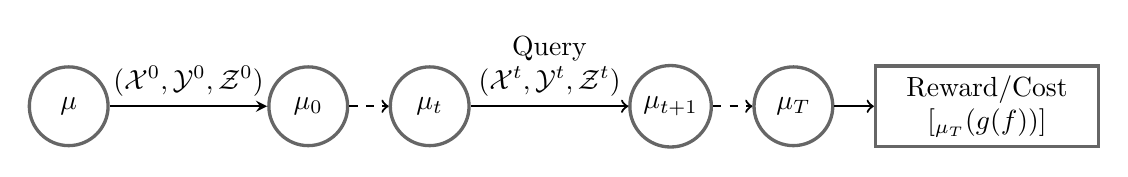
\begin{tikzpicture}
[
roundnode/.style={circle, draw=black!60, very thick, minimum size=10mm},
squarednode/.style={rectangle, draw=black!60, very thick, minimum size=10mm, align =center,text width = 26mm},
]
%Nodes
\node[roundnode]      (maintopic)                              {$\mu$};
\node[roundnode]        (circle1)       [right=20mm of maintopic] {$\mu_0$};
\node[roundnode]      (circle2)       [right=5mm of circle1] {$\mu_t$};
\node[roundnode]        (circle3)       [right=20mm of circle2] {$\mu_{t+1}$};
\node[roundnode]        (circle4)       [right=5mm of circle3] {$\mu_T$};
\node[squarednode]        (circle5)       [right=5mm of circle4] {Reward/Cost $\E \left[ \V_{\mu_T} (g(f))\right]$};


%Lines
\draw[thick, ->, >=stealth] (maintopic.east) -- node[anchor=south] {$(\mathcal{X}^0,\mathcal{Y}^0,\mathcal{Z}^0)$} (circle1.west);
\draw[thick, ->, dashed] (circle1.east) --  (circle2.west);
\draw[thick, ->] (circle2.east)  -- node[above, align =center, text width = 18mm] { Query $(\mathcal{X}^t,\mathcal{Y}^t,\mathcal{Z}^t)$} (circle3.west);
\draw[thick, ->,dashed] (circle3.east) --  (circle4.west);
\draw[thick, ->] (circle4.east) --  (circle5.west);


\end{tikzpicture}
\caption{MDP framework for adaptive labeling to efficiently estimate the average treatment effect (ATE).}
\label{fig:MDP_framework_flowchart}
\end{figure}
 









\begin{comment}
\subsection{Broader applicability of the framework to other problem settings} \label{sec:broad-framework-accuracy}
 

Although  we describe our setting in a healthcare setting with the objective  to estimate the recall of a trained AI model $\model(\cdot)$, the framework caters to many other problem settings. The extension to the evaluation of model based on accuracy (in regression setting) is straightforward, we simply replace the definition of recall $g(f)$ in~\eqref{eqn:l2-g-f} with
\begin{align*}
    g(f) = \E_{\substack{ y \sim p(y|f,x) \\  \forall x \in \mathcal X}} \big( \E_{{\textbf x} \sim p_x} [y-\model(x)]^2 \big).
\end{align*}


\textcolor{red}{To discuss if we need to have it here}
We can also extend this setting to the efficient estimation of the ATE as well. We describe these in detail below:

\begin{itemize}
    
    \item Estimating accuracy:  \[g(f) = \E_{\substack{ y \sim p(y|f,x) \\  \forall x \in \mathcal X}} \big( \E_{{\textbf x} \sim p_x} [y-\model(x)]^2 \big)\]
%    \item Estimating ATE with known control arm: 
%\[g(f) = \E_{\substack{ y \sim p(y|f,x) \\  \forall x \in \mathcal X}} \big( \E_{{\textbf x} \sim p_x} [y-\model(x)] \big)\]
\item Estimating ATE  (with minor modifications - broad structure remains similar) : 


Consider feature vector ${\mathbf x} \in \mathcal X $  distributed as ${\mathbf x}  \sim p_{\mathbf x}$, treatment $z \in {\mathcal Z} = \{0,1\}$, and a class of random functions $f: {\mathcal X} \times {\mathcal Z} \to {\mathcal Y}$, which determines the likelihood $p(y_i|f,{\mathbf x_i},z_i)$. Note that $f$ is random and reflects our uncertainty about how
labels are generated given features and the treatment. Additionally, the joint likelihood is determined as follows,  

\[p(Y|f,X,Z) = \prod_{i} p(y_i|f,{\mathbf x_i}, z_i) \]

Assuming the prior over functions $f$ to be $\mu$, therefore we have 
\[p(Y|X,Z) = \int \prod_{i} p(y_i|f,{\mathbf x_i},z_i) d\mu(f) \]


Also, assuming that under the  true data generating function $f$ (if known precisely - which we don't), the estimand of interest is

\[ \E_{{\textbf x} \sim p_x}  \left( \E_{\substack{ y \sim p(y|x,f,z=1) }} y - \E_{\substack{ y \sim p(y|x,f,z=0) }} y \right) \]


Throughout the paper we assume the above data generating process.  Now, suppose we have some labeled  data $(\datax^0,\datay^0,Z^0) =({\mathbf x}_{1:m}^0,y_{1:m}^0, z_{1:m}^0)$. 
    We run a experiment, in which we want to query the labels (in batches), so as to minimize the uncertainty of the estimand of interest. Suppose, the horizon of the experiment is $T$. Now, given prior $\mu$ and labeled data $\datax^0,\datay^0,Z^0$, in the beginning of our experiment the posterior state is $\mu_0$.

 At each step $j$ ($j \geq 1$), we query labels for a batch (with size $k$) of unlabeled data $(\datax^j,Z^j) \subset \mathcal X \times \mathcal Z$  and get labels $\datay^j$. After acquiring the labels at each step $j$ we update posterior state to $\mu_{j+1}$, informed by $\mu_j$ and $(\datax^j,\datay^j,Z^j)$. 
 
 Let the policy at step $j$ be $\pi_j$ (potentially random), which gives $\datax^{j+1},Z^{j+1} \sim \pi_j(\mu_j)$.  Observe that $\mu_{j+1}$ is random because of the randomness of the policy $\pi_j$ and $\datay^{j+1}|\{\datax^{j+1},Z^{j+1},\mu_j\}$ (\textcolor{red}{can this be written in a better way?}). Let, $\pi = \{\pi_0,....,\pi_{T-1}\}$. Therefore, our objective is to

 
\[ \min_{\pi} \E \left[ {\mathbf {Var}}_{f \sim \mu_T} \left( \E_{{\textbf x} \sim p_x}  \left( \E_{\substack{ y \sim p(y|x,f,z=1) }} y - \E_{\substack{ y \sim p(y|x,f,z=0) }} y \right) \right) \right]\]

where, $\mu_T$ depends on $\{(\datax^i,\datay^i,Z^i)\}_{i=0}^T$ and outer expectation is over both $\pi$ and  $\datay^{j+1}|\{\datax^{j+1}, Z^{j+1},\mu_j\}$ for all $j \in [0,T-1]$.


%Constraining the action space is straightforward - by first choosing set of x's using k-subset and then assigning treatment with learnable probability parameters $w_1,...,w_n$.

\end{itemize}

 \[ g(f) = \E_{\substack{ y \sim p(y|f,x) \\  \forall x \in \mathcal X}}\E_{{\textbf x} \sim p_x} g(y,{\textbf x}) \approx \E_{\substack{ y \sim p(y|f,x) \\  \forall x \in  \datax^u}} \left( \frac{1}{n}\sum_{i=1}^n \tilde{g}(y,{\textbf x}_i^u) \right)\]




Notation borrowed from a combination of the following papers 
~\citep{LeeYuNaFoLe23, KatoOgKoIn24, FongHoWa24}

%  
\end{comment}


%%% Local Variables:
%%% mode: latex
%%% TeX-master: "main"
%%% End:
     
\subsection{Evaluation metrics}
\label{sec:UQ_eval_metrics}

%Typical approaches in uncertainty quantification (UQ) posit latent factor models that determines the prior and the likelihood. These latent factors, being unobserved, present a challenge in justifying the relative validity of one model over another. Instead, we view UQ models as outputting a probability distribution over a number of data points given contexts, which allows us to evaluate UQ models based on their ability to explain held-out observed sequences. This view is well-founded in  prequential statistics~\citep{Roberts65,Dawid84}, sequence modeling view of Bayesian models~\citep{FortiniPe23}, and information theory~\citep{BarronRiYu98}. Most recently,~\citet{OsbandWeAsSeDwLuVa22} propose this approach to evaluating UQ models.
 Recall we denoted by $ \mc{D}^{0} = (\mc{X}^{0}, \datay^{0}) := (X_{1:m-1},Y_{1:m-1})$ the initial training data and let $X_i \simiid Q_X$. Further, let $P_X$ be the distribution we expect to see during deployment and  $\mc{X}^{0} $ only represents a part of this distribution (with having selection bias). 
 Also recall, given a true data generating function  $f\opt$, outcomes $Y$ are generated as following:
\begin{equation*}
    Y = f\opt(X) + \varepsilon.
\end{equation*}
for some random noise $\varepsilon$,
We view UQ models as outputting a probability distribution over a number of data points given contexts, which allows us to evaluate UQ models based on their ability to explain held-out observed sequences. 
This view is well-founded in  prequential statistics~\citep{Roberts65,Dawid84}, sequence modeling view of Bayesian models~\citep{FortiniPe23}, and information theory~\citep{BarronRiYu98}.
Most recently,~\citet{OsbandWeAsSeDwLuVa22} propose this approach to evaluating UQ models.
Suppose we wish to predict $\tau$ outcomes 
$\ypred \defeq \ypredsetl$ for features $\xpred \defeq \xpredsetl$ where $\xpredsetl \simiid P_X$. The corresponding true outcomes are $y_{m+1:m+\tau}$.  Further, let $\mu(f|\mc{D}^0)$ be the posterior from some UQ module after seeing data $\mc{D}^0$. We  set our evaluation metric to be

\begin{align}
- \log {\left[\int \left(\prod_{i=m}^{m+\tau} p_\epsilon (y_i -f(X_i))\right) d\mu(f|\mc{D}^0) \right]}.
\label{joint_log_loss}
\end{align}




%Let $\dtrain \defeq \dtrainsetl$ be the training data, where $X_i \simiid P_X$ is a feature vector in $\R^d$ and $Y_i \in \R$ is the label/ outcome.  where $\varepsilon$ is a mean zero noise independent of everything else. $Y_i$'s are i.i.d. conditional on $U$ and $X_i$, but linked through the latent factor $U$. If the class of regression functions $\{ f\opt(\cdot, u): u \in \mbox{supp}(U)\}$ was well-specified, then any uncertainty due to $U$ is fully resolvable in the limit of infinite observations. For this reason, we refer to stochasticity due to $U$  epistemic / actionable uncertainty and that due to $\varepsilon$ aleatoric / irreducible uncertainty.

% We wish to predict $\tau$ outcomes 
% $\ypred \defeq \ypredsetl$ for features $\xpred \defeq \xpredsetl$. Based on prior knowledge and data $\dtrain$ generated by a particular realization of $U$,
% we view UQ modules as estimating the 
% $\tau$-sequence probability $p(\ypredsetl \in \cdot ~ |U,\xpredsetl)$ with $\what{p}(\ypredsetl \in \cdot ~ |\xpredsetl)$.

% Recall we denoted  $\mu_0(\cdot) = \mu(f\mid \mc{D}^0)$, the posterior state after observing data $\mc{D}^0$.




% The KL divergence between the oracle and predicted sequence probabilities provides a natural performance measure
% \begin{align}
% & \E_{X_i \simiid P_X, U \sim \pi}
% \left[\dkl{p(\ypredsetl \in \cdot ~ |U,\xpredsetl)}{\what{p}(\ypredsetl \in \cdot ~ |\xpredsetl)}
% \right] \nonumber \\
% & \qquad \qquad \propto
% - \E_{X_i \simiid P_X, U \sim \pi, Y_i = f\opt(X_i, U) + \varepsilon}
% \left[\log  \what{p}(\ypredsetl |\xpredsetl) \right].
% \label{eqn:joint-log-loss}
% \end{align}

% Since the $Y_i$'s in the preceding display are coupled via the latent factor $U$,
\citet{OsbandWeAsSeDwLuVa22}~referred to the above metric as ``\emph{marginal} log-loss'' when 
$\tau=1$ and as ``\emph{joint} log-loss'' when $\tau > 1$. Marginal log-loss represents the expected negative log-likelihood of predicting a single test example, based on the UQ module’s predictive distribution for that specific input. On the other hand, joint log-loss is defined as the expected negative log-likelihood for a batch of test examples, calculated under the model’s joint predictive distribution across various label combinations for the entire batch of inputs. This effectively provides a unified measure to compare the performance of UQ methods. 
%The significance of joint log-loss was also emphasized by~\citep{OsbandWeAsDwLuIbLaHaDoRo22}. 


 
% For example, an idealized Bayesian approach posits a class of models $\{\what{f}(\cdot, u): u \in \mc{U}\}$ that approximates the model class $\{ f\opt(\cdot, u): u \in \mbox{supp}(U)\}$ and generate ``posterior predictives'' $\what{p}(\ypredsetl = \ypredset ~ |\xpredsetl)$ via
% \begin{align}
% \label{eqn:ppd}
% \int \what{p}(\ypredsetl = \ypredset \mid \xpredsetl, u) \what{\pi}(u) du := \int \prod_{i=1}^\tau 
%  \what{p}_{\varepsilon}\left(y_i - \what{f}(X_i, u)\right)
%  \what{\pi}(u) du,
% \end{align}
% where $\what{p}_{\varepsilon}$ is an estimator of
% the likelihood (pdf of $\varepsilon$) and $\what{\pi}(\cdot) := \what{\pi}(\cdot; \mc{D}^0)$ is the prior estimated based on the initial data $\mc{D}^0$.



% Variational inference-based Bayesian neural networks (BNNs)~\citep{JospinLaBoBuBe22},  %. 
% %This category encompasses techniques such as 
%  dropout~\citep{GalGh16}, Bayes by Backprop~\citep{BlundellCoKaWi15}, and Ensembles/ Ensemble $+$~\citep{LakshminarayananPrBl17,OsbandAsCa18}
%  can be represented with the above abstraction.
% BNNs model $\what{f}(X, U)$ a neural network with weights $U \sim \what{\pi}$ and input $X$.
% Ensembles typically consider discretely supported $U \sim \what{\pi}$, where $\what{f}(X, u)$ is 
% a predictive model trained on a (bootstrapped) subset of the training data for $u = \{1, ..., K\}$.
% %\hntodo{I don't know how to write ENNs in my abstraction. @Daksh, please rewrite the below paragraph in the new notation.}
% ~\citet{OsbandWenAsDwIbLuRo23} propose Epistemic Neural Networks (ENNs) and showed that they outperform traditional BNNs at a much lower computational cost. ENNs also fall under the above Bayesian framework and consider a set of functions $\set{g_\eta(\cdot,u): u}$, where $\eta$ is a fixed  parameter  
% and $u$ is called epistemic index with an associated  distribution.

\paragraph{Joint log-loss with dyadic sampling} 
To evaluate the quality of joint predictions as discussed, batches of inputs $(X_1, \cdots, X_\tau)$ need to be sampled multiple times, and their log-loss is assessed against corresponding labels $(y_1, \cdots, y_\tau)$. 
Typically, batch size $\tau$ required to effectively distinguish joint predictions that reflect label interdependencies becomes large as dimensionality of data increases, and it becomes impractical as dimension increases. 
Dyadic sampling~\citep{OsbandWeAsDwLuIbLaHaDoRo22} offers a practical heuristic to estimate joint likelihood.
The basic dyadic sampling method starts by independently sampling two anchor points, $X_1$ and $X_2$, from the input distribution. Then, $\tau$ points are sampled independently and with equal probability from these two anchor points $\set{X_1, X_2}$ that leads to a random sample $X_{(1)}, \cdots, X_{(\tau)}$.
An agent's joint prediction of labels is evaluated on this batch of size $\tau$.  In our experiments, we use $\tau = 10$ and it seems to be an effective estimator of the joint log-loss.



\paragraph{In-distribution and out-of-distribution evaluations} If training distribution and prediction distribution are same, that is $Q_X =P_X$, then we call it in-distribution performance. If $Q_X \neq P_X$  then it is the case of distribution shifts (potentially out-of-support).



\section{\label{sec:method}Methodology}

Each SIEM system uses its own RDL to define threat detection rules, and each RDL has its own schema.
For example, the Splunk SIEM uses the SPL to define its threat detection rules.
The task of understanding threat detection rules and recommending relevant MITRE ATT\&CK techniques (or sub-techniques) requires complex reasoning skills.
In the case of LLMs, this can be achieved with a technique called prompt chaining in which each task is divided into multiple sub-tasks in order to understand the complex reasoning behind the task.
Therefore, we employ a multi-phase architecture based on prompt chaining that leverages the power of LLMs to take a SIEM rule defined in any RDL and map it to relevant MITRE ATT\&CK techniques using the power of LLMs.
Our approach is based on the following intuitions:
\begin{itemize}[nosep,leftmargin=*]
    \item \textit{LLMs' implicit knowledge}: LLMs possess deep understanding of diverse RDLs. This enables them to interpret any rule, regardless of the RDL it is defined in, and convert it into comprehensible natural language text.
    \item \textit{LLMs' similarity comparison capability}: LLMs are adept at analyzing and comparing textual descriptions. 
    They can intelligently assess the similarity between two textual inputs to establish a meaningful connection.
\end{itemize}

\methodName has two main phases: (1) the rule to text translation phase, and (2) the MITRE ATT\&CK techniques recommendation phase.
These two phases in the pipeline include six key steps to determine relevant TTPs, as illustrated in Figure~\ref{fig:r2t}.

Although LLMs excel at translating SIEM rules into natural language, they often lack critical domain-specific contextual information related to IoCs in the rules.
To overcome this limitation, the \textit{rule to text translation} phase includes three steps: IoC extraction, contextual information retrieval, and natural language translation.

The workflow begins with the extraction of IoCs from the rules (for example, processes, log source, event codes, and file names) that the rule searches for in the logs (step (1)).In the next sstep a web search agent performs the task of obtaining additional contextual information about the IoCs discovered ((step 2)).
By incorporating this additional domain-specific information, the pipeline enhances the language translation, resulting in a more accurate and meaningful interpretation of SIEM rules.
The rule itself and the IoCs' contextual additional information from the previous stage are then used to translate the rule from RDL to natural language (step (3)).

The \textit{MITRE ATT\&CK techniques} recommendation phase of the pipeline includes the following three steps.
The rule in processed in data source identification step in which the probable origin of the data is identified (step (4)).
The description of the rule is then used to determine probable MITRE ATT\&CK techniques based on the implicit knowledge of the LLM (step (5)).
Finally, using chain-of-thought~\cite{wei2022chain} prompting, the most relevant techniques are extracted from the list of probable techniques (step (6)).
Each step of our method is further described in detail below.


% [bb=0 0 1440 900,width=1.43\linewidth,height=0.9\textwidth]
\begin{figure*}[htbp]
   \includegraphics[width=\textwidth]{Images/stages.jpg}
    
   \caption{An illustration of the different steps in \methodName.}
   \label{fig:stages}
\end{figure*} 

\subsection{IoC Extraction}
The context associated with a SIEM detection rule is crucial for its accurate interpretation and effective application. 
Obtaining this contextual understanding requires comprehensive analysis of the embedded IoCs in the SIEM rule.
In the first step, \methodName systematically identifies and extracts all IoCs, identifying the types of IoCs and their corresponding values that form the foundational elements of the detection rules. 
Leveraging the LLM's inherent understanding of rule structures and IoCs, we employ a zero-shot prompting approach for this task. 
Zero-shot prompting enables the direct extraction of IoCs from the rules without requiring extensive pre-training on specific datasets.

\noindent The result of this stage is a dictionary structure, where:
\begin{itemize}[nosep,leftmargin=*]
    \item Keys represent types of IoC, such as processes, files, IP addresses, and log sources.
    \item Values are lists containing specific IoC details, such as process names, file names, IP addresses, and log source identifiers.
\end{itemize}

In the example depicted in Figure~\ref{fig:stages}(a), the pipeline processes a rule for which relevant MITRE ATT\&CK techniques need to be recommended. 
The IoC extractor LLM produces a dictionary structure as output, organizing the IoCs in a structured format to support subsequent stages in the analysis pipeline. 



\subsection{Contextual Information Retrieval}
In this step, an LLM agent is employed to retrieve relevant information pertaining to the IoCs extracted from the rule.
A REACT agent~\cite{react} was used in this case to generate both reasoning traces and task-specific actions in an interleaved manner.
REACT agents interact with external tools to retrieve additional information that leads to more factual and reliable responses.
The LLM agent conducts a systematic search across web resources to gather additional contextual information for each IoC value present in the rule. 
This step addresses LLMS' lack of up-to-date knowledge or specialized domain expertise (which is critical to understanding the role and significance of the IoCs in the rule), without the need for retraining or fine-tuning.
Figure~\ref{fig:stages}(b) presents an example in which the rule includes the process name \texttt{soaphound.exe} as an IoC.
As can be seen, the web search results indicate that \texttt{soaphound.exe} is being used for active directory (AD) enumeration, which is important for the understanding of the attack. 

\subsection{Natural Language Translation}

The translation of detection rules into natural language textual descriptions fulfills three key objectives:
\begin{enumerate}[nosep,leftmargin=*]
    \item \textbf{Ensures that \methodName is format-agnostic}: It converts rules defined in various RDL formats into a generic, unstructured text format, ensuring compatibility with different SIEM systems, regardless of the specific rule format.
    \item \textbf{Provides contextual explanation}: It includes all relevant contextual information to produce a concise and comprehensible explanation of the rule.
    \item \textbf{Enhances the comprehension for LLMs}: It enables LLMs to more effectively compare the translated rule with descriptions in the MITRE ATT\&CK framework by providing a unified textual representation.
\end{enumerate}
To achieve these objectives, a zero-shot prompting technique is employed. 
The input to the LLM comprises two components:
\begin{itemize}
    \item \textbf{Syntactical information}: The rule itself, providing the structural and operational details.
    \item \textbf{Contextual information}: Details of the IoCs extracted from the rule, providing semantic insights into the rule's intent and function.
\end{itemize}
The LLM utilizes these inputs to generate a natural language textual description of the rule. 
This transformation not only ensures a more interpretable representation but also facilitates further steps of analysis and comparison, particularly in aligning the rule with MITRE ATT\&CK techniques and sub-techniques.



\subsection{Data Source or Mitigation Identification}
Identifying the most relevant data component or mitigation associated with the rule description in this step is critical for filtering out irrelevant MITRE ATT\&CK techniques (or sub-techniques) in subsequent steps of the pipeline.
In the MITRE ATT\&CK framework, data sources represent various categories of information that can be gathered from sensors or logs. 
These data sources include \textit{data components}, which are specific attributes or properties within a data source that are directly relevant to detecting a particular technique or sub-technique~. 
For example, in the context of the rule described in Figure~\ref{fig:stages}(a), the term \texttt{Endpoint.Processes} indicates that the activity is happening on an endpoint. 
Presence of the terms such as, \texttt{soaphound.exe}, \texttt{--buildcache}, \texttt{--certdump} and etc. indicate that the rule searches for command line execution of an executable named \texttt{soaphound.exe} with specific parameters. 
Therefore, the appropriate data source in this example is \textit{Command}, with the corresponding data component being \textit{Command Execution}.
Additionally, \textit{mitigations} are defined as categories of technologies or strategies that can prevent or reduce the impact of specific techniques or sub-techniques. 
The MITRE ATT\&CK framework explicitly establishes relationships between data components, mitigations, and techniques (or sub-techniques), enabling a systematic approach for identifying relevant elements.

To identify the most relevant data component or mitigation associated with a given rule description, we utilize agentic retrieval augmented generation (RAG), which incorporates an AI Agent-based implementation of the RAG framework.
Data from the MITRE ATT\&CK framework, specifically related to data components and mitigations, is stored in a vector database (e.g., ChromaDB). 
The process begins with the rule description from the previous stage, which serves as the input to the AI Agent. 
The LLM-powered agent automatically generates a search query tailored to retrieve relevant information from the RAG database.

For each query, the system retrieves the five most similar documents from the database, each containing contextual information about data components or mitigations. 
These documents are then utilized by the LLM agent to contextualize the rule description. 
By comparing the content of these retrieved documents with the rule description, the LLM agent determines and outputs the most relevant data component or mitigation along with a chain-of-thought as to why the data component or mitigation is related to the rule.


\subsection{Probable Technique Recommendation}

In this step, an LM agent is utilized to propose probable MITRE ATT\&CK techniques (and sub-techniques) that may be relevant to the description of the provided rule.
We used a REACT agent in this step as well to utilize both implicit and explicit knowledge during reasoning.
For explicit knowledge, the agent searches the MITRE ATT\&CK framework to obtain the list of probable techniques (and sub-techniques).
The natural language description of the rule from the previous step serves as input to the LLM agent.
The output of this stage consists of a list of JSON objects, each containing the MITRE technique ID, technique name, and technique description as seen in Figure~\ref{fig:stages}(c).

Throughout our experiments, we observed that as the number of recommendations ($k$) increases, both the framework's average recall and precision initially improve, however beyond a certain threshold of $k$, the %average 
precision begins to decline.
Based on these observations(please refer Table~\ref{tab:results3}), we selected a $k$-value of 11 to ensure a high recall.



\subsection{Relevant Technique Extraction}
In this step, \methodName refines the set of probable MITRE ATT\&CK techniques identified in the previous stage by eliminating irrelevant entries.
This step in the pipeline serves two primary purposes: (1) to enhance precision while maintaining recall achieved in previous step, and (2) to provide a clear rationale for the selection of the labels, ensuring transparency and interpretability of the mapping process.
This refinement process is grounded in the assumption that LLMs are effective for text similarity matching tasks.

The process comprises two key steps:
\begin{itemize}
    \item \textit{Rule-technique comparison}: The description of each technique in the set of probable techniques is compared with the rule description. 
    A chain-of-thought technique is then applied to elucidate the reasoning behind the association of each technique with the rule.
    \item \textit{Confidence calculation}: The generated chain-of-thought rationale for each technique (or sub-technique) is compared with the rule description to compute a relevance (or confidence) score, as done in prior work~\cite{freitas2024ai}.
    % \item \textbf{Reasoning}: \new{Add here the reasoning that it provides - explaining in NLP why it was selected...}
\end{itemize}

Techniques with higher confidence scores are deemed more relevant to the rule. 
Conversely, techniques with scores falling below a predefined threshold are excluded.
The techniques retained after this filtering step represent the most relevant techniques corresponding to the given rule's description. 


The chain-of-thought (CoT) rationale generated during the comparison of each rule to its probable technique is also provided as an output in this step.
This rationale offers a detailed natural language explanation, articulating why a particular technique is relevant to the given rule. 
Such explanations are highly valuable for security analysts, as they provide clear and transparent reasoning behind the mapping, enabling analysts to better understand and validate the association between the rule and the technique.
Other classification models proposed in previous works within this domain also suffer from the limitation of being black-box models, which lack the ability to provide clear reasoning or explanations. 
Unlike \methodName, these models fail to generate transparent, CoT rationales that explain why a particular rule is mapped to a specific technique, making them less interpretable and less useful for security analysts.     
Frontier language models demonstrate a remarkable mismatch between their problem-solving capabilities and poor out-of-box verification capabilities.
These limitations have largely been attributed to the inability of current language models to self-diagnose hallucinations or enforce rigour \citep{zhang_how_2023,orgad_llms_2024,snyder_early_2024,kamoi_evaluating_2024, tyen_llms_2024, DBLP:conf/iclr/0009CMZYSZ24}.
However, our findings that models can be directed to accurately perform verifications at scale suggest that these out-of-box limitations can be addressed with standard methods like instruction tuning.
We compiled a set of challenging reasoning problems and candidate solutions to provide a benchmark for these deficits.

Each entry in this benchmark consists of a question, a correct candidate response, and an incorrect candidate response, and is manually curated from the residuals of our sampling-based search experiments (Section~\ref{section:pipeline}).
An example entry from this benchmark can be found below (see Appendix~\ref{app:examplebenchmark} for more).

\vspace{0.4cm}
\begin{tcolorbox}[title=Question from LiveBench Reasoning (Web-of-Lies Puzzle), breakable]
In this question, assume each person either always tells the truth or always lies. The person at the campground thinks their friend is lying. Mateo is at the aquarium. The person at the restaurant says the person at the hotel lies. Farid is at the movie theater. The person at the movie theater says the person at the campground lies. Ryan is at the shopping mall. The person at the cafe says the person at the campground lies. The person at the observatory says the person at the museum lies. The person at the museum says the person at the restaurant tells the truth. The person at the campground says the person at the airport tells the truth. The person at the campground tells the truth. Luna is at the restaurant. The person at the movie theater saw a firetruck. Isabella is at the observatory. The person at the amusement park says the person at the museum tells the truth. The person at the restaurant says the person at the shopping mall tells the truth. Liam is at the beach. Ayaan is at the airport. The person at the restaurant says the person at the beach tells the truth. Maya is at the amusement park. The person at the restaurant says the person at the aquarium lies. The person at the restaurant says the person at the movie theater lies. The person at the library says the person at the campground tells the truth. Elowen is at the hotel. Priya is at the library. The person at the gym says the person at the restaurant tells the truth. Kehinde is at the cafe. Anika is at the museum. Quan is at the campground. Soren is at the gym. Does the person at the museum tell the truth? Does the person at the restaurant tell the truth? Does the person at the movie theater tell the truth? Think step by step, and then put your answer in **bold** as a list of three words, yes or no (for example, **yes, no, yes**). If you don't know, guess.
\end{tcolorbox}
\definecolor{mydarkgreen}{rgb}{0.0, 0.5, 0.0} %


\begin{paracol}{2}

\switchcolumn[0]
\begin{tcolorbox}[breakable, colframe=mydarkgreen!70, colback=mydarkgreen!10, title=Correct response]
Here's how we can break down this logic puzzle:

1. **Quan is at the campground and tells the truth.** This is a given fact.

...

4. **The person at the restaurant (Luna) says the person at the hotel (Elowen) lies.**  We don't know yet if Luna is lying or telling the truth.

...

10. **Since Luna tells the truth about Farid, Luna *always* tells the truth.**  This unlocks several other pieces of information.

...

13. **The person at the cafe (Kehinde) says the person at the campground lies.** Since Quan tells the truth, Kehinde is lying.

Therefore:
* **Anika (museum):** Tells the truth.
* **Luna (restaurant):** Tells the truth.
* **Farid (movie theater):** Lies.

**yes, yes, no**
\end{tcolorbox}

\switchcolumn
\begin{tcolorbox}[breakable, colframe=red!70, colback=red!10, title=Incorrect Response Due to Hallucination]
Here's how we can solve this logic puzzle:

1. **Quan is at the campground and tells the truth.** This is given.

2. **The person at the airport (Ayaan) tells the truth.** Quan (campground) says the person at the airport tells the truth, and Quan tells the truth.

...

4. **Luna (restaurant) lies.**  The person at the restaurant says the person at the hotel (Elowen) lies. \textbf{\color{red} Later, the person at the restaurant says the person at the campground (Quan) lies.} Since Quan tells the truth, Luna (restaurant) must be lying.

...

Therefore:
* **Anika (museum): lies**
* **Luna (restaurant): lies**
* **Farid (movie theater): lies**

**Answer: no, no, no** 
\end{tcolorbox}
\end{paracol}

\noindent\begin{minipage}{\textwidth}
\captionof{figure}{Example of an entry in our verification benchmark. The question is sourced from the LiveBench Reasoning benchmark, and the two responses are generated by Gemini v1.5 Pro. The green response has the correct final answer; the red response has the wrong final answer due to hallucinating a non-existent clause.}
\label{fig:example}
\vspace{0.4cm}
\end{minipage}

\noindent
On each entry, our benchmark studies verification accuracy on two tasks:
\begin{enumerate}
    \item \textbf{Scoring task.} When given only the question and one of the responses, is the model able to discern the correctness of the response?
    \item \textbf{Comparison task.} When provided the whole tuple with the correctness labels of the responses masked and a guarantee that at least one response is correct, is the model able to discern which response is correct and which is incorrect?
\end{enumerate}

\noindent
The scoring task is also evaluated over a separate set of (question, response) pairs where the response reaches the correct final answer by coincidence but contains fatal errors and should be labeled by a reasonable verifier as being incorrect; an example can be found in Appendix~\ref{app:examplebenchmark}.
In the scoring task, models are provided only with the task description; in the comparison task, models are provided only with the task description and a suggestion to identify disagreements between responses in its reasoning.

Table~\ref{tab:benchmark} lists the baseline performances of current commercial model offerings on this benchmark.
Gemini v1.5 Pro is omitted from the benchmark as the entries in the benchmark are curated from the residuals of Gemini v1.5 Pro.
The prompts used in Table~\ref{tab:benchmark} are provided in Appendix~\ref{app:benchmarkprompts}.

As we previously observed, and has been noted in prior works \citep{tyen_llms_2024, kamoi_evaluating_2024}, verification errors are typically due to low recall.
Even the easier comparison task, models perform only marginally better---and often worse---than random chance.
In many cases, Consistency@5 performs worse than one-shot inference because Consistency simply averages out noise from an output distribution, meaning that a model biased towards producing an incorrect answer will do so with higher probability under Consistency.
Addressing these deficits in verification capabilities---which we see as low-hanging fruit for post-training---would enable not only better sampling-based search, but also other downstream applications of verification including reinforcement learning \citep[e.g.][]{o1-preview,deepseekai2025deepseekr1incentivizingreasoningcapability}, data flywheeling \citep[e.g.,][]{welleck_generating_2022}, and end-user experience (see Section~\ref{sec:related} for further discussion).


\begin{table}[htbp]
\centering
\begin{tabular}{llcccccc}
\toprule
\textbf{Model} & \textbf{Metric} & \multicolumn{3}{c}{\textbf{Scoring Accuracy}} & \multicolumn{1}{c}{\textbf{Comparison Accuracy}} \\
\cmidrule(lr){3-5} \cmidrule(lr){6-6}
 &  & \textbf{Correct} & \textbf{Wrong} & \textbf{Flawed} &  \\
\midrule
\multirow{2}{*}{GPT-4o} & Pass@1    & 76.5\%  & 31.0\% & 22.2\% & 43.2\%\\
 & Consistency@5 & 77.4\% & 30.0\% & 11.1\% & 35.4\% \\
\midrule
\multirow{2}{*}{Claude 3.5 Sonnet} & Pass@1 & 89.6\% & 22.5\% & 33.3\% & 56.1\% \\
 & Consistency@5 & 90.3\% & 17.5\% & 33.3\% & 61.2\% \\
\midrule
\multirow{2}{*}{o1-preview} & Pass@1 & 100\% & 68.8\% & 80.0\% & 84.5\% \\
 & Consistency@5 & 100\% & 79.4\% & 88.8\% & 92\% \\
\midrule
\multirow{2}{*}{Gemini 2.0 Flash} & Pass@1 & 73.5\% & 44.5\% & 60\% & 58\%  \\
 & Consistency@5 & 77.4\% & 42.5\% & 66.6\% & 58.7\% \\
\midrule
\multirow{2}{*}{Gemini 2.0 Thinking Flash} & Pass@1 & 75.4\% & 56.5\% & 53.3\%  & 80\%  \\
 & Consistency@5 & 77.4\%  & 55\% & 55.5\%  & 89.1\% \\
\midrule
\multicolumn{2}{c}{Random guessing}  & 80\% & 20\% & 20\% & 50\% \\
\bottomrule
\end{tabular}
\caption{Accuracy rates of commercial language models on our verification benchmark. For the task of response scoring (Scoring Accuracy), accuracy rates are broken down for entries that require identifying a correct response as being correct (Correct), entries that require identifying a wrong response as being wrong (Wrong), and entries that require identifying a wrong response that coincidentally reaches the correct answer as being wrong (Flawed).
GPT-4o and Claude 3.5 Sonnet only perform marginally better than random guessing across all tasks. o1-Preview performs better, but still fails to identify 20-30\% of wrong responses.
}
\label{tab:benchmark}
\end{table}

\section{Experiments: Planning outperforms Heuristics}
\label{sec:experiment}

We begin our empirical demonstrations by showcasing the effectiveness of our planning framework on both synthetic and real datasets. We focus on the simplest planning algorithm, 1-step lookaheads (Algorithm~\ref{alg:complete}), and show that even basic planning can hold great promise. 
We illustrate our framework using two uncertainty quantification modules---GPs and 
\ensembles/ \ensembleplus. 

Throughout this section, we focus on evaluating the mean squared error of 
a regression model $\model$,  and develop adaptive policies that minimize uncertainty on $g(f)$ defined in~\eqref{eqn:l2-g-f}.
When GPs provide a valid model of uncertainty, 
our experiments show that our planning framework significantly outperforms other baselines. 
We further demonstrate that our conceptual framework extends to deep learning-based uncertainty quantification methods such as  \ensembleplus while highlighting computational challenges that need to be resolved in order to scale our ideas. 
For simplicity, we assume a naive predictor, i.e., $\psi(\cdot) \equiv 0$. However, we emphasize that this problem is just as complex as if we were using a sophisticated model $\psi(.)$. The performance gap between the algorithms 
primarily depends
on the level  of uncertainty in our prior beliefs.

To evaluate the performance of our algorithm, we benchmark it against several baselines. 
%Active learning baselines use an acquisition function $\ac$ to select points that have the highest   function value: $X\opt_t \in \argmax_{X \in \xpoolj{t}} \ac({X})$ at every step $t$. These methods may also need an UQ module, which we simply use the same UQ module as in our algorithm, and it  outputs $V(X)$ that measures the the uncertainty of each point $X \in \xpoolj{t}$.
Our first set of baselines are from active learning~\citep{AggarwalKoGuHaPh14}:
\\ % \noindent\textbf{Active Learning Heuristics:} 
\textbf{(1)} 
\textsf{Uncertainty Sampling (Static):}  In this approach, we query the samples for which the model is least certain about. Specifically, we estimate the variance of the latent output $f(X)$ for each $X \in \xpool$ using the UQ module and select the top-$K$ points with the highest uncertainty. \\
\textbf{(2)} \textsf{Uncertainty Sampling (Sequential):} This is a greedy heuristic that sequentially selects the points with the highest uncertainty within a batch, while updating the posterior beliefs using pseudo labels from the current posterior state. Unlike \textsf{Uncertainty Sampling (Static)}, this method takes into account the information gained from each point within batch, and hence tries to diversify the selected points within a batch. 

 
We also compare our approach to the  \textbf{(3)} \textsf{Random Sampling}, which selects each batch uniformly at random from the pool. Additionally, we compare solving the planning problem using  \textsf{REINFORCE}-based policy gradients with   $\mathsf{Smoothed\text{-}Autodiff}$ policy gradients.\footnote{Our code repository is available at
  \url{https://github.com/namkoong-lab/adaptive-labeling}.}
%Detailed experimental setups are provided in Section \ref{sec:details-experiments}.

%We repeat all experiments with 10 random seeds.




\begin{figure}[t]
\centering
\begin{minipage}[b]{0.49\textwidth}
\centering
\includegraphics[width=\textwidth, height=5cm]{figures/original_scale/Var_of_l_2_loss.pdf}
\caption{(Synthetic data) Variance of mean squared loss evaluated through the posterior belief $\mu_t$ at each horizon $t$. This is the objective that policy gradient methods like \textsf{REINFORCE} and $\ouralgo$ optimizes. 1-step lookaheads are surprisingly effective even in long horizons.}
\label{fig:var-l2-sim}
\end{minipage}
\hfill
\begin{minipage}[b]{0.49\textwidth}
\centering \includegraphics[width=\textwidth, height=5cm]{figures/original_scale/Error_of_estimated_model_l_2_loss.pdf}
\caption{(Synthetic data) Error between MSE calculated based on collected data $\mc{D}^{0:T}$ vs. population oracle MSE over $\mc{D}_{\rm eval} \sim P_X$. Reducing uncertainty over posteriors directly leads to better OOD evaluations. 1-step lookaheads significantly outperform active learning heuristics in small horizons.}
\label{fig:mean-l2-sim}
\end{minipage}
%\caption{Simulated data for GPs}
%\label{fig:both_plots}
\end{figure}

\subsection{Planning with Gaussian processes}
\label{sec:experiment-plan-GP}
We now briefly describe the data generation process for the GP experiments,  deferring a more detailed discussion of the dataset generation to Section~\ref{sec:details-experiments}. 
We use both the synthetic data and the real data to test our methodology.
For the \emph{simulated data},  we construct a setting where the general population is distributed across \emph{51 non-overlapping clusters} while the initial labeled data $\dtrain$ just comes from one cluster. In contrast, both $\dpool \defeq (\xpool,\ypool),\deval \defeq (\xeval,\yeval)$ are generated   from all the clusters. 
We begin with a low-dimensional scenario, generating a one-dimensional regression setting using a GP. %Gaussian Process (GP).
Although the data-generating process is not known to the algorithms,  we assume that the GP hyperparameters are known to all the algorithms
to ensure fair comparisons. This can be viewed as a setting where our prior is well-specified, allowing us to isolate the effects
of different policy optimization approaches
 without any concerns about the misspecified priors. We select $10$ batches, each of size $K=5$ across $T = 10$ time horizons.

To examine the robustness of our method against the distributional assumptions made  in the simulated case, we then move to a real dataset where the correct prior is not known. We simulate selection bias from the eICU dataset~\citep{PollardJoRaCeMaBa18}, which contains real-world patient data with in-hospital mortality outcomes. 
We conduct a $k$-means clustering to generate 51 clusters and then select data from those clusters. We view this to be a credible replication of practice, as severe distribution shifts are common due to selection bias in clinical labels.  To convert the binary mortality labels into a regression setting, we train a  random forest classifier and fit a GP on predicted scores, which serves as the UQ module for all the algorithms. As before, the task is to select 10 batches, each consisting of 5 samples, across 10 time horizons.

 In Figures~\ref{fig:var-l2-sim} and~\ref{fig:mean-l2-sim}, we present results for the simulated data. 
Figure~\ref{fig:var-l2-sim} shows the variance of $\ell_2$ loss, and Figure~\ref{fig:mean-l2-sim} presents the error in the estimated $\ell_2$ loss using $\mu_t$ (relative to true $\ell_2$ loss, that is unknown to the algorithm). 
As we can see from these plots, our method one-step lookahead  gives substantial improvements  over active learning baselines and random sampling. In addition,
compared to the one-step lookahead planning approach using \textsf{REINFORCE}-based policy gradients, 
we observe that $\mathsf{Smoothed\text{-}Autodiff}$-based policy gradients provide significantly more robust performance over all horizons.

In Figures~\ref{fig:var-l2-real}~and~\ref{fig:mean-l2-real}, we observe similar findings on the eICU data. We see that planning policies (\textsf{REINFORCE} and $\mathsf{Smoothed\text{-}Autodiff}$) consistently outperform other heuristics by a large margin.  Active learning baselines perform poorly in these small-horizon batched problems and can sometimes be even worse than the random search baselines.  Overall, our results show the importance of careful planning in adaptive labeling for reliable model evaluation. 

We offer some intuition as to why one-step lookahead planning may outperform other heuristic algorithms. 
 First,  \textsf{Uncertainty sampling (Static)} while myopically selects the
 top-$K$ inputs with the highest uncertainty, it fails to consider 
the overlap in information content among the ``best” instances; see \citep{AggarwalKoGuHaPh14} for more details. 
In other words,  it might acquire points from the same region with high uncertainty while failing to induce diversity among the batch.
Although \textsf{Uncertainty Sampling (Sequential)} somewhat addresses the issue of information overlap, a significant drawback of 
this algorithm
is the disconnect between the objective we aim to optimize and the algorithm. For example, it might sample from a region with high uncertainty but very low density. 

\begin{figure}[t]
\centering
\begin{minipage}[b]{0.48\textwidth}
\centering
\includegraphics[width=\textwidth, height=5cm]{figures/original_scale/Var_of_l_2_loss_real.pdf}
\caption{(Real-world eICU data) Variance of mean squared loss evaluated through the posterior belief $\mu_t$ at each horizon $t$. Even 1-step lookaheads are extremely effective planners, and auto-differentiation-based pathwise policy gradients provide a reliable optimization algorithm based on low-variance gradient estimates.}
\label{fig:var-l2-real}
\end{minipage}
\hfill
\begin{minipage}[b]{0.48\textwidth}
\centering \includegraphics[width=\textwidth, height=5cm]{figures/original_scale/Error_of_estimated_model_l_2_loss_real.pdf}
\caption{(Real-world eICU data) Error between MSE calculated based on collected data $\mc{D}^{0:T}$ vs. population oracle MSE over $\mc{D}_{\rm eval} \sim P_X$. Reducing uncertainty over posteriors directly leads to better OOD evaluations. Our method significantly outperforms active learning-based heuristics, and random sampling.}
\label{fig:mean-l2-real}
\end{minipage}
%\caption{Real data for GPs}
\end{figure}
 
%\vspace{-1.5cm}
% \begin{wrapfigure}{r}{.32\columnwidth}
%   \vspace{-.5cm} 
%   \centering
% \includegraphics[scale=.29]{figures/Var of l2l_2 loss.pdf}
%   \vspace{-0.2cm}
%   \caption{Results of GP}
% \label{fig:var-l2-gp}
%   \vspace{-0.1cm}
% \end{wrapfigure}


% Attempts have been made  in the past to address these  drawbacks heuristically  (see \citep{AggarwalKoGuHaPh14}). We give a unified computational framework while approaching the problem in a more principled manner and solving it more optimally.




\subsection{Planning with  neural network-based uncertainty quantification methods ($\ensembleplus$)}


We now provide a proof-of-concept that shows the generalizability of our conceptual framework  to the deep learning-based UQ modules, specifically focusing on $\ensembleplus$ due to their previously observed superior performance~\citep{OsbandWenAsDwIbLuRo23}. Recall that implementing our framework with deep learning-based UQ modules  requires us to retrain the model across multiple possible random actions $\bm{a}(\theta)$ sampled from the current policy $\pi_\theta$.
This requires significant computational resources, in sharp contrast to the GPs where the posteriors are in closed form and can be readily updated and differentiated. 

Due to the computational constraints, we test $\ensembleplus$ on a toy setting to demonstrate the generalizability of our framework. We consider a setting where the general population consists of four clusters, while the initial labeled data only comes from one cluster. Again we generate data using GPs.  The task is to select a batch of 2 points in one horizon. We detail the $\ensembleplus$ architecture in Section \ref{sec:details-experiments}, and we assume prior uncertainty to be large (depends on the scaling of the prior generating functions). 
The results are summarized in the Table~\ref{tab:UQ_ensemble}.

% \begin{table}[H]
% \vspace{-10pt}
% \caption{Performance under \ensembleplus as UQ module}
%     \centering
%     \begin{tabular}{|m{3cm}|m{2.5cm}|m{2cm}|} 
%     \hline
%       Algorithm   & Variance of $\loss_2$ loss estimate & Error of $\loss_2$ loss estimate  \\ \hline Random Sampling 
%          & $1710.9 \pm 1352.1$ & $8.67\pm6.62$ 
%       \\ \hline \ouralgo & $1.30 \pm 0.68$ & $0.91\pm0.25$ \\ \hline
%     \end{tabular}
%     \label{tab:UQ_ensemble}
%     %\vspace{-10pt}
% \end{table}




\begin{table}[h]
\vspace{-10pt}
\caption{Performance under \ensembleplus as the UQ module}
\centering
\begin{tabular}{|l|l|l|}
\hline
Algorithm   & Variance of $\loss_2$ loss estimate & Error of $\loss_2$ loss estimate  \\
\hline
\textsf{Random sampling} & 7129.8 $\pm$ 1027.0 & 136.2 $\pm$ 8.28 \\ \hline
\textsf{Uncertainty sampling (Static)} & 10852 $\pm$ 0.0 & 162.156 $\pm$ 0.0 \\ \hline
\textsf{Uncertainty sampling (Sequential)} & 8585.5 $\pm$ 898.9 & 144 $\pm$ 6.93 \\ \hline
\textsf{REINFORCE} & 1697.1 $\pm$ 0.0 & 45.27 $\pm$ 0.0 \\ \hline
\ouralgo & 1697.1 $\pm$ 0.0 & 45.27 $\pm$ 0.0 \\ \hline
\end{tabular}
%\caption{Comparison of different algorithms based on variance   and   error in $\ell_2$ loss estimation with Ensemble $+$ as the UQ module. Our results demonstrate that {\ouralgo} and REINFORCE outperformthe other active learning based heuristics, confirming the benefits of our MDP formulation for the adaptive labeling problem, as also demonstrated in Section 4.\\
%\footnotesize{Experimental details: We use Gaussian Processes as our data generating process, GP parameters are the same as in Section D.3.  The task is to select a batch of 2 points along one horizon.The marginal distribution $p_X$ has 4 \textit{non-overlapping} clusters. Initial data comes from one cluster, while pool and evaluation points comes from all the clusters. We have $20$ initial labeled data points, $10$ pool points, and $252$ evaluation points.  Training procedures are similar to the one in Section D.3.} }
\label{tab:UQ_ensemble}
\end{table}



% We faced  issues in scaling up these experiments which will be our focus in the future. 





% \begin{itemize}
%     \item Posteriors should be consistent. Two dimensions: even with less training,  
%     \item the inference should be  fast enough
% \end{itemize}


% Potential research directions for uncertainty quantification

% In this section we consider a simple setting We consider a simpler setting and 


% For synthetic dataset generation, we use ...... For real datasets, we use ...... We compare our methodolgy to several baselines ()    This Section is structured as follows:
% \begin{itemize}
%     \item \textbf{GPs, square loss objective} (Section \ref{}): 
%     %the broad aim of the experiments  in this section is to isolate the performance of our methodology without any concerns for the inefficiencies induced due to a mis-specified prior or imperfect posterior inference. To accomplish this we generate synthetic datasets using GPs (detailed later). We use the well specified prior (GPs - with same hyperparameter setting) as our UQ module.   
%      As GPs provide differentaible posterior inference - any errors induced due to imperfect posterior updates are also isolated. We note that under this setting
%      \item In Section\ref{} we demonstrate why our methodology performs better than other baselines - by devising various synthetic experiments ()
%     \item  \textbf{UQ Benchmarking }(Section \ref{}): Before diving into the experiments using $\ensembleplus$ and ENNs,  we showcase our benchmarking experiments in Section \ref{}. We use real datasets We observe that ENNs perform better
%      \item \textbf{Ensemble $+$}, objective: recall, accuracy
%     \item \textbf{ENN}, objective: recall, accuracy
% \end{itemize}




% In Section {}, we test 
% \subsection{Experimental details}

% \begin{itemize}
%     \item UQ methodologies - GPs, ENNs
%     \item Objectives - Recall,  ATE
%     \item Datasets - ATE-synthetic datasets, Recall-synthetic, real datasets
%     \item Baselines - 
%     \begin{itemize}
%         \item Random sampling
%         \item Active learning - Uncertainty based sampling - In regression setting almost all of the 
%         \item Myopic greedy - Greedy Batch based sampling
%         \item Policy Gradient
%     \end{itemize}
    
% \end{itemize}

% \subsection{Experiments}
%     \begin{itemize}
%     \item GPs with square loss
%     \item Benchmarking ENN
%         \item ENNs with ATE
%         \item ENNs with Recall
%     \end{itemize}

% \subsection{Benefits over other algorithms - intuition and experiments}

%Active learning - Myopic greedy / Don't rely on the objective rather some entropy version.


%%% Local Variables:
%%% mode: latex
%%% TeX-master: "main"
%%% End:
    
\section*{Conclusion}
This paper aims to enhance our understanding of the computational complexity of computing various Shapley value variants. We found that for various ML models --- including decision trees, regression tree ensembles, weighted automata, and linear regression --- both local and global interventional and baseline SHAP can be computed in polynomial time under HMM modeled distributions. This extends popular algorithms, such as TreeSHAP, beyond their empirical distributional scope. We also establish strict complexity gaps between the various SHAP variants (baseline, interventional, and conditional) and prove the intractability of computing SHAP for tree ensembles and neural networks in simplified scenarios. Overall, we present SHAP as a versatile framework whose complexity depends on four key factors: \begin{inparaenum}[(i)] \item model type, \item SHAP variant, \item distribution modeling approach, \item and local vs. global explanations\end{inparaenum}. We believe this perspective provides deeper insight into the computational complexity of SHAP, paving the way for future work.




%We believe that our framework provides a more intricate understanding of SHAP computation complexity across different models, distributions, and variants, paving the way for further research.

Our work opens promising directions for future research. First, expanding our computational analysis to other SHAP-related metrics, such as asymmetric SHAP~\citep{frye20} and SAGE~\citep{covert2020understanding}, would be valuable. Additionally, we aim to explore more expressive distribution classes and relaxed assumptions beyond those in Section \ref{sec:tractable} while maintaining tractable SHAP computation. Finally, when exact computation is intractable (Section \ref{sec:intractable}), investigating the approximability of SHAP metrics through approximation and parameterized complexity theory~\citep{downey2012parameterized} is an important direction.

%Our work opens several promising avenues for future research on the computational properties of explainable AI methods, with a particular focus on SHAP. First, it would be interesting to broaden the computational analysis conducted in this work to include other popular SHAP-related metrics in the literature, such as asymmetric SHAP \cite{frye20} and SAGE \cite{covert2020understanding}. Also, in the future, we aim to explore more expressive distribution classes and relaxed distributional assumptions—extending beyond those examined in Section \ref{sec:tractable} —that still yield tractable SHAP computation. Finally, when exact computation proves intractable (Section \ref{sec:intractable}), it is worthwhile to theoretically investigate the question of the approximability of computing the SHAP metrics across various configurations, through the lens of approximation and parametrized complexity theory \cite{arora2009computational}.

%This paper aims to deepen our understanding of the computational complexity involved in obtaining different Shapley value variants. We found that for a variety of ML models, including decision trees, tree ensembles for regression, weighted automata, and linear regression models — computing both local and global interventional and baseline SHAP can be done in polynomial time when distributions are modeled by HMMs. This extends the distributional scope of popular algorithms like TreeSHAP, which is limited to empirical distributions. Additionally, we demonstrate a strict complexity gap between SHAP variants, showing that interventional and baseline SHAP can be strictly easier to compute than conditional SHAP. Despite these positive results, we uncovered intractability for various SHAP variants in neural networks and tree ensembles. Finally, we provided generalized complexity relations across SHAP variants. We believe that our framework offers a deeper understanding of the complexity involved in computing SHAP across various variants, models, distributions, as well as in both local and global computations, laying the groundwork for future research.


%\input{UQ/details_dataset}


%While Gaussian processes works well in low dimensions,  quantifying epistemic uncertainty on $f\opt(Y|X)$  over high dimensional inputs is an active area of research, including popular techniques such as dropout~\citep{GalGh16}, Bayes by Backprop~\citep{BlundellCoKaWi15}, Ensembles/Ensemble++~\citep{LakshminarayananPrBl17,OsbandAsCa18}, hypermodels~\citep{DwaracherlaLuIbOsWeVa20} and Epistemic Neural Networks \citep{OsbandEtAl23}. Our framework is compatible with deep learning-based uncertainty quantification models such as ensembles where we can only do approximate posterior updates. 


%To overcome the computational issue of Ensembles/Ensemble+~\citep{LakshminarayananPrBl17,OsbandAsCa18},  ENNs were proposed and shown to outperform Ensembles at a much lower computational cost. For synthetic data, we use GP as an oracle and compare other UQ modules with it.






 





% \subsubsection{Bayes by Backprop (BBB)~\citep{BlundellCoKaWi15}:} is an efficient way of obtaining approximate posterior by minimizing the KL divergence between the approximate and
% true posterior and using a 
% reparameterization trick.


% \subsection{Metric:}
% \label{sec:joint-log-loss}

% \textbf{Joint log loss}: Following~\citep{WenOsQiLuIbDwAsVa22,OsbandWeAsSeDwLuVa22,OsbandEtAl23}, we consider joint log loss.


% \subsection{Our codebase}\label{sec:out-code-base}


% Our code is available at \url{https://anonymous.4open.science/r/UQBench-CD51}. As we mentioned earlier we build over the neural testbed benchmark~\citep{OsbandWeAsDwLuIbLaHaDoRo22} for our code base.  We provide more details  in the README file  in the repository.
\section{Experimental details (Section \ref{sec:experiment})} \label{sec:details-experiments}

In this section, we provide detailed information about the experiments discussed in Section~\ref{sec:experiment}. 

\subsection{Planning with Gaussian Processes - synthetic data experiments}

As mentioned earlier, we generate our data using a  Gaussian Process ({GP}). Specifically, we use a {GP} with an RBF kernel: $f_i \sim \mathcal{GP}(m,\mc{K}) $, where $m(X)=0$ and $\mc{K}(X,X') = \sigma_f^2 \exp\left(-\frac{||X-X'||_2^2}{2\loss^2}\right)$, further Gaussian   noise $N(0,\sigma^2)$ is added to the outputs. We set $\loss = 1$, $\sigma_f^2 = 0.69$, and $\sigma^2 = 0.01$.
Recall that the marginal distribution $P_X$ consists of $51$ \textit{non-overlapping} clusters. To achieve this, we create a polyadic sampler, which first samples $51$ anchor points spaced at linearly increasing distances from the center to avoid overlap. These anchor points serve as our cluster centers. We sample the points around these anchor points by adding a small Gaussian noise $N(0,0.25)$. The training points are drawn from a single cluster, while the pool and evaluation points are drawn from all the $51$ clusters. The setup includes $100$ initial labeled data points, $500$ pool points and $285$ evaluation points used to estimate the objective. 

\noindent\textbf{\ouralgo~ training and hyperparameters:} As mentioned earlier, the underlying uncertainty quantification (UQ) module for these experiments is the {GP}. Although our algorithm does not know the true data generating function, but it has access to the {GP} hyperparameters. Therefore we use a $\mathcal {GP}$ with an RBF kernel: $f_i \sim \mathcal{GP}(m,\mc{K}) $, where $m(X)=0$ and $\mc{K}(X,X') = \sigma_f^2 \exp\left(-\frac{||X-X'||_2^2}{2\loss^2} \right)$, with 
Gaussian   noise $N(0,\sigma^2)$ added to the outputs. We set $\loss = 1$, $\sigma_f^2 = 0.69$ and $\sigma^2 = 0.01$. For soft $K$-subset sampling  (see Algorithm~\ref{alg:k-subset}),  we set $\tau$ to $0.1$. Further for evaluating the objective function $\V (g(f))$ - we take $100$ samples of $f(\xeval)$ from the posterior state $\mu_+^{a(\theta)}$. 
For policy optimization in each horizon, we use the Adam optimizer with a learning rate of $0.1$ to perform policy gradient steps over $100$ epochs. The results presented are averaged over $10$ different training seeds.


\noindent\textbf{Policy gradient (\rein) training and hyperparameters:} As mentioned earlier, all the algorithms have access to the true to {GP} hyperparameters. For evaluating the objective $\V (g(f))$ under a given action,  we take $100$ samples of $f(\xeval)$.  To optimize the policy in each horizon, we use the Adam optimizer with a learning rate of $0.1$ to perform policy gradient updates over $100$ epochs. The results presented are averaged over $10$ different training seeds.


\subsection{Planning with Gaussian Processes - real data (eICU) experiments}


The eICU  dataset is a healthcare dataset that contains data from various critical care units across the United States. To create a supervised learning setup from this dataset, we first extracted the $10$ most important features using a \texttt{Random Forest} classifier (number of trees $=$ $100$, criterion $=$ ``gini'').  The outcome variable was in-hospital mortality. Some examples of the extracted features include: Hospital length of stay, Number of days on the ventilator and the Last recorded temperature on Day 1 of ICU admission. We transformed the classification outcome variable (in-hospital mortality) into a regression task using the probability of in-hospital mortality predicted by the classifier.
To adapt the extracted data to our setting, we introduced selection bias in the data. We generated 51 clusters through the standard $k-$means algorithm. Our initial labeled data comes from only $1$ cluster, while the pool and evaluation data comes from all the $51$ clusters. Our dataset consists $100$ initial labeled data points, $500$ pool points, and $285$ evaluation points used to estimate the objective. 


We then fitted a  {GP}  with an RBF kernel to above data using  {GP}-regression. The resulting {GP} hyperparameters were: $m(x)=0.255$, $\loss = 0.50, \sigma_f^2 = 1.0, \sigma^2 =0.0001$. This $\mathcal{GP}$ model serves as our uncertainty quantification (UQ) module.


\noindent\textbf{\ouralgo  ~ training and hyperparameters:} For soft $K$-subset sampling  (see Algorithm~\ref{alg:k-subset}),  we set $\tau$ to $0.1$. Further to evaluate the objective function $\V (g(f))$, we take 100 samples of $f(\xeval)$ from the posterior state $\mu_+^{a(\theta)}$.
For policy optimization in each horizon, we use the Adam optimizer with a learning rate of $0.1$ to perform policy gradient steps over $1000$ epochs. The results presented are averaged over $10$ different training seeds.


\noindent\textbf{Policy gradient (\rein) training and hyperparameters:} To evaluate the objective $\V (g(f))$ under an action, we take $100$ samples of $f(\xeval)$.  For optimizing the policy in each horizon, we use an Adam optimizer with learning rate of $0.1$,  performing policy gradient updates over $1000$ epochs. The results presented are averaged over $10$ different training seeds.



\subsection{Planning with \ensembleplus experiments}

  Once again, we use {GP}s as our data generating process. Specifically, we use a GP with an RBF kernel: $f_i \sim \mathcal{GP}(m,\mc{K}) $, where $m(X)=0$ and $\mc{K}(X,X') = \sigma_f^2 \exp\left(-\frac{||X-X'||_2^2}{2\loss^2} \right)$. Additionally, Gaussian noise   $N(0,\sigma^2)$ is added to the outputs. We set $\loss = 1$, $\sigma_f^2 = 0.69$, and $\sigma^2 = 0.01$.
The marginal distribution $P_X$ consists of $4$ \textit{non-overlapping} clusters. We follow the same process as in the Gaussian process experiments to form the cluster centers and sample points around them. While the training points are drawn from a single cluster, both the pool and evaluation points are drawn from all the $4$ clusters. Our setup includes $20$ initial labeled data points, $10$ pool points, and $252$ evaluation points used to evaluate the objective. 

%\footnotesize{Experimental details: We use Gaussian Processes as our data generating process, GP parameters are the same as in Section D.3.  The task is to select a batch of 2 points along one horizon.The marginal distribution $p_X$ has 4 \textit{non-overlapping} clusters. Initial data comes from one cluster, while pool and evaluation points comes from all the clusters. We have $20$ initial labeled data points, $10$ pool points, and $252$ evaluation points.  Training procedures are similar to the one in Section D.3

\noindent\textbf{\ensembleplus Architecture:} We use an ensemble of 10 models. Each model being a 2-hidden layer MLP with 50 units per hidden layer. In addition, each models includes an additive prior. The additive prior function for each model is fixed to be a 2-hidden layer MLP with 50 units in each hidden layer.  
 Specifically, the $m$-th model for $1\leq m \le 10$ of the \ensembleplus takes the form
\begin{align*}
    f_{\eta_m}(X) = g_{\eta_m}(X) + \alpha p_m(X),
\end{align*}
where $g_{\eta_m}$  is the trainable part of the network while $\alpha p_m(\cdot)$ is the additive prior function. Here $\alpha$ controls our prior belief about the uncertainty ---higher the $\alpha$, the greater the uncertainty. The prior functions $p_m(\cdot)$ differ across models $m$ due to different initializations. In our setup, we set $\alpha=100$ to reflect a high level of uncertainty in the prior beliefs.




\noindent\textbf{\ensembleplus training:} For a given dataset ${\mathcal D} =(X_i,Y_i)_{i=1}^n$, we train the $m$-th model so as to minimize the following loss function 
\begin{align*}
    \loss(\eta_m, \mathcal D) =  \frac{1}{n}\sum_{i=1}^n (g_{\eta_m}(X_i) + \alpha p_m(X_i)-Y_i)^2 + \lambda \norm{\eta_m}_2^2.
\end{align*}
We tune $\lambda$ to $0.1$ and use the Adam optimizer with a tuned learning rate of $0.1$. Each model is trained for 50 iterations.
%Although in standard \ensembleplus, each model is trained on a different bootstrapped subset from the dataset ${\mathcal D}$, in our case we train all the models  within \ensembleplus on the entire dataset available.



 
\noindent\textbf{\ouralgo  ~ training and hyperparameters:} Recall that in soft $K$-subset sampling there is a hyperparameter $\tau$  (see Algorithm~\ref{alg:k-subset}), which we set to $0.1$. To differentiate through the argmin operation, we employ the differentiable optimizer from the $\mathsf{torchopt}$ package, specifically the MetAdam Optimizer with a learning rate of $0.1$. For optimizing the sampling policy, we use the Adam optimizer with a learning rate of $0.05$, performing policy gradient updates over $500$ epochs. 




% \begin{table}[H]
% \vspace{-10pt}
% \caption{Performance under \ensembleplus as UQ module}
%     \centering
%     \begin{tabular}{|m{3cm}|m{2.5cm}|m{2cm}|} 
%     \hline
%       Algorithm   & Variance of $\loss_2$ loss estimate & Error of $\loss_2$ loss estimate  \\ \hline Random Sampling 
%          & $1710.9 \pm 1352.1$ & $8.67\pm6.62$ 
%       \\ \hline \ouralgo & $1.30 \pm 0.68$ & $0.91\pm0.25$ \\ \hline
%     \end{tabular}
%     \label{tab:UQ_ensemble_old}
%     %\vspace{-10pt}
% \end{table}

%\colorbox{pink}{${\mathbb E} [\V_{\mu_0} (g(f))]$}


%\colorbox{pink}{${\mathbb E} [\V_{\mu_2} (g(f))]$}



%\colorbox{pink}{${\mathbb E} [\V_{\mu_t} (g(f))]$}


%\definecolor{customgray}{gray}{0.85} % Lighter gray

%\colorbox{customgray}{Pick $\{{\mathcal X^1}:\subseteq \xpoolj{1} \}$}

%\colorbox{customgray}{Pick $\{{\mathcal X^2}:\subseteq \xpoolj{2} \}$}

%\colorbox{customgray}{Pick $\{{\mathcal X^t}:\subseteq \xpoolj{t} \}$}

 
%The chosen hyperparameters for different experiments are available in our code base. 





%
% For Figure~\ref{fig:task-1-joint-ood-all-data},  we train different methodologies for 5000 iterations for eICU-Linear Bias dataset. For eICU-clustering bias dataset and synthetic dataset we train methodologies for 200 iterations as training dataset is now of smaller size. The results presented are average over 10 different inference and test batch seeds. 


% For syenthetic datasets,
% we perform hyperparameter sweeps over the following sets for each agent:
% \begin{itemize}
%     \item For \textbf{mlp}, we sweep over learning rate in $\{0.001\}$, training iterations in $\{20, 50, 100, 200\}$, and L2 weight decay in $\{10\}$.
%     \item For \textbf{dropout}, we sweep over learning rate in $\{0.001\}$, training iterations in $\{20, 50, 100, 200\}$, length scale in $\{0.1\}$, and dropout rate in $\{0.2\}$.
%     \item For \textbf{ensemble}, we sweep over learning rate in $\{0.001\}$, training iterations in $\{20, 50, 100, 200\}$, and L2 weight decay in $\{0.01\}$.
%     \item For \textbf{ensemble+}, we sweep over learning rate in $\{0.001\}$, training iterations in $\{20, 50, 100, 200\}$, L2 weight decay in $\{0.01\}$, and prior scale in $\{30\}$.
%     \item For \textbf{hypermodel}, we sweep over learning rate in $\{0.001\}$, training iterations in $\{20, 50, 100, 200\}$, L2 weight decay in $\{0.01\}$, and prior scale in $\{100\}$.
%     \item For \textbf{epinet}, we sweep over learning rate in $\{0.001\}$, training iterations in $\{20, 50, 100, 200\}$, L2 weight decay in $\{0.1\}$, and prior scale in $\{0.1\}$.
% \end{itemize}

%\ym{we need more parameters sweep}


% \subsection{The hyperparamters we choose}

% %\dm{How many seeds in the Figure 23 and 21}
% \dm{How many seeds for the other graphs}
%\dm{Mention that this standard deviation will go away if we can compute in the closed form}

%\subsection{Details  for synthetic data}



 


 

\subsubsection{Comparison with a Gaussian oracle}
In synthetic data generation setting we compare different UQ methodologies to the  Gaussian process oracle baseline with access to the parameters of the the data generation process (which is also an GP).  Figure~\ref{fig:task-1-joint-ood-all-data-with-oracle} compares  different UQ methodolgies and the GP oracle (the setting is same to that in Figure~\ref{fig:task-1-joint-ood-all-data}).
From Figure~\ref{fig:task-1-joint-ood-all-data-with-oracle}, we observe that UQ methodology ``GP'', which is the oracle, performs better for a large $k$, and for small $k$ values, many other UQ methodlogies are quite similar in performance. 

\begin{figure}
\centering 
\centering \includegraphics[height=4.5cm]{figures/GP_dynamic_0/Task_1_kl_estimate_dyadic_tau_10_ood_vs._k_val_for_num_batches=250_dynamic_0_with_oracle.pdf}

\centering{\small{ Synthetic Data (Clustering bias)}}
\caption{Joint log-loss on OOD data with increasing selection bias with a GP oracle.}
\label{fig:task-1-joint-ood-all-data-with-oracle}
\end{figure}


\subsubsection{Hyperparameter tuning breaks under distribution shifts}

\label{sec:hyperparameter_tuning_breaks_under_dis_shifts_experiment_simple}

Figure~\ref{fig:difficult_to_choose_weight_decay} demonstrates that increasing the weight decay deteriorates ID performance while first improving OOD performance and subsequently deteriorating.  
Similarly, Figure~\ref{fig:difficult_to_choose_stopping_time} shows that as number of iterations increases, ID performance improves on the test set.  On the other hand, test OOD performance first improves with increasing training iterations but later deteriorates for \ensembleplus and Hypermodels.




\begin{figure}[h]
\centering
\begin{minipage}[b]{0.32\textwidth}
\centering
\includegraphics[height=4.5cm]{figures/eicu_clustering/Experiment_2_weight_decay_ensemble+_with_500_training_iterations.pdf}

\centering {\small{\ensembleplus}}
%\label{fig:ensemble+_difficult_to_choose_weight_decay}
\end{minipage}
\hfill
\begin{minipage}[b]{0.32\textwidth}
\centering \includegraphics[height=4.5cm]{figures/eicu_clustering/Experiment_2_weight_decay_epinet_with_500_training_iterations.pdf}
\centering {\small{Epinet}}
%\label{fig:epinet_difficult_to_choose_weight_decay}
\end{minipage}
\hfill
\begin{minipage}[b]{0.32\textwidth}
\centering \includegraphics[height=4.5cm]{figures/eicu_clustering/Experiment_2_weight_decay_hypermodel_with_500_training_iterations.pdf}
\centering {\small{Hypermodel}}
%\label{fig:hypermodel_difficult_to_choose_weight_decay}
\end{minipage}
\caption{Trade-off between  in-distribution (ID) and out-of-distribution (OOD) performance with weight decay as the hyperparameter (eICU, Clustering bias). }
\label{fig:difficult_to_choose_weight_decay}
\end{figure}




    






\begin{figure}[h]
\centering
\begin{minipage}[b]{0.31\textwidth}
\centering
\includegraphics[height=4cm, width=\textwidth]{figures/eicu_clustering/Task_1_ood_id_ensemble+_Metric_vs._Number_of_Batches_for_k_val=30_dynamic_0.pdf}
\centering {\small{\ensembleplus}}
\label{fig:ensemble+_difficult_to_choose_stopping_time}
\end{minipage}
\hfill
\begin{minipage}[b]{0.31\textwidth}
\centering \includegraphics[height=4cm, width=\textwidth]{figures/eicu_clustering/Task_1_ood_id_epinet_Metric_vs._Number_of_Batches_for_k_val=30_dynamic_0.pdf}
\centering {\small{Epinet}}
\label{fig:epinet_difficult_to_choose_stopping_time}
\end{minipage}
\hfill
\begin{minipage}[b]{0.31\textwidth}
\centering \includegraphics[height=4cm, width=\textwidth]{figures/eicu_clustering/Task_1_ood_id_hypermodel_Metric_vs._Number_of_Batches_for_k_val=30_dynamic_0.pdf}
\centering {\small{Hypermodel}}
\label{fig:hypermodel_difficult_to_choose_stopping_time}
\end{minipage}
\caption{Trade-off between  in-distribution (ID) performance and out-of-distribution (OOD) performance with stopping time as the hyperparameter (eICU, clustering).}
\label{fig:difficult_to_choose_stopping_time}
\end{figure}
    


\subsubsection{Dynamic settings for   other datasets}


To further examine our findings in Figure~\ref{fig:dynamic_setting_k_30}, we conduct similar experiments using clustering bias as described in Section~\ref{sec:selection-bias} for all datasets in Section~\ref{sec:UQ_BENCH_datasets}.
We summarize our results in Figure~\ref{fig:dynamic_setting_IEEECIS}
for \ieeecis, Figure~\ref{fig:dynamic_setting_ccfraud}
for \ccfraud, Figure~\ref{fig:dynamic_setting_fraudecom}
for \fraudecom,  Figure~\ref{fig:dynamic_setting_vehicleloan}
for \vehicleloan,  Figure~\ref{fig:dynamic_setting_ACS_employment}
for \acsemployment, and 
Figure~\ref{fig:dynamic_setting_ACSincome_NY_}
for \acsincome. 
In summary, our results are consistent with the results from Figure~\ref{fig:dynamic_setting_k_30}. 
Interestingly, we observe some UQ agents can actually have a larger joint log-loss after adapting to new data.
 





\begin{figure}[h]
\centering
\begin{minipage}[b]{0.24\textwidth}
\centering
\includegraphics[width = \textwidth, height=2.5cm]{figures/new_data/IEEECIS_in_distribution_mean_T0.pdf}
{\small{{(a)} ID performance ($T=0$) }}
\end{minipage}
\hfill
\begin{minipage}[b]{0.24\textwidth}
\centering \includegraphics[width = \textwidth, height=2.5cm]{figures/new_data/IEEECIS_out_of_distribution_mean_T0.pdf}
{\small{{(b)} OOD performance ($T=0$) }}
\end{minipage}
\hfill
\begin{minipage}[b]{0.24\textwidth}
\centering \includegraphics[width = \textwidth, height=2.5cm]{figures/new_data/IEEECIS_out_of_distribution_mean_T50.pdf}
{\small{{(c)} OOD performance ($T=1$) }}
\end{minipage}
\hfill
\begin{minipage}[b]{0.24\textwidth}
\centering \includegraphics[width = \textwidth, height=2.5cm]{figures/new_data/IEEECIS_out_of_distribution_mean_difference.pdf}
{\small{{(d)} OOD improvement ($T=0 \to 1$) }} \end{minipage}
\caption{Performance of different UQ modules in a dynamic setting for \ieeecis.
Although Hypermodels perform the best in the ID setting (a), they perform the worst in the OOD setting at $T=0$. However, we see that Hypermodels are good at adapting to new data for this dataset and quickly improve the performance as shown in plot (d).
}
\label{fig:dynamic_setting_IEEECIS}
\end{figure}


\begin{figure}[h]
\centering
\begin{minipage}[b]{0.24\textwidth}
\centering
\includegraphics[width = \textwidth, height=2.5cm]{figures/new_data/ccfraud_in_distribution_mean_T0.pdf}
{\small{{(a)} ID performance ($T=0$) }}  
\end{minipage}
\hfill
\begin{minipage}[b]{0.24\textwidth}
\centering \includegraphics[width = \textwidth, height=2.5cm]{figures/new_data/ccfraud_out_of_distribution_mean_T0.pdf}
{\small{{(b)} OOD performance ($T=0$) }} 
\end{minipage}
\hfill
\begin{minipage}[b]{0.24\textwidth}
\centering \includegraphics[width = \textwidth, height=2.5cm]{figures/new_data/ccfraud_out_of_distribution_mean_T50.pdf}
{\small{{(c)} OOD performance ($T= 1$) }} 
\end{minipage}
\hfill
\begin{minipage}[b]{0.24\textwidth}
\centering \includegraphics[width = \textwidth, height=2.5cm]{figures/new_data/ccfraud_out_of_distribution_mean_difference.pdf}
{\small{{(d)} OOD improvement ($T=0 \to 1$) }} 
\end{minipage}
\caption{Performance of different UQ modules in a dynamic setting for \ccfraud. 
In this case hypermodels perform the best for both the ID setting (a) and the OOD setting (b) at $T=0$. However, we can see that the OOD performance improvement (d) is the best for the epinets, which again showcases the trade-off between having sharper posteriors and the performance on the  OOD data.}
\label{fig:dynamic_setting_ccfraud}
\end{figure}


\begin{figure}[h]
\centering
\begin{minipage}[b]{0.24\textwidth}
\centering
\includegraphics[width = \textwidth, height=2.5cm]{figures/new_data/fraudecom_in_distribution_mean_T0.pdf}
{\small{{(a)} ID performance ($T=0$) }} 
\end{minipage}
\hfill
\begin{minipage}[b]{0.24\textwidth}
\centering \includegraphics[width = \textwidth, height=2.5cm]{figures/new_data/fraudecom_out_of_distribution_mean_T0.pdf}
{\small{{(b)} OOD performance ($T=0$) }} 
\end{minipage}
\hfill
\begin{minipage}[b]{0.24\textwidth}
\centering \includegraphics[width = \textwidth, height=2.5cm]{figures/new_data/fraudecom_out_of_distribution_mean_T50.pdf}
{\small{{(c)} OOD performance ($T=1$) }} 
\end{minipage}
\hfill
\begin{minipage}[b]{0.24\textwidth}
\centering \includegraphics[width = \textwidth, height=2.5cm]{figures/new_data/fraudecom_out_of_distribution_mean_difference.pdf}
{\small{{(d)} OOD improvement ($T=0 \to 1$) }} 
\end{minipage}
\caption{Performance of different agents in a dynamic setting for \fraudecom. Surprisingly, we observe that all three models have a larger OOD joint log-loss after seeing new data. The reason for such a behaviour might be that the models start from a prior belief with lower level of uncertainty and as they see additional data they become more uncertain. }
\label{fig:dynamic_setting_fraudecom}
\end{figure}

\begin{figure}[h]
\centering
\begin{minipage}[b]{0.24\textwidth}
\centering
\includegraphics[width = \textwidth]{figures/new_data/vehicleloan_in_distribution_mean_T0.pdf}
{\small{{(a)} ID performance ($T=0$) }} 
\end{minipage}
\hfill
\begin{minipage}[b]{0.24\textwidth}
\centering \includegraphics[width = \textwidth, height=2.5cm]{figures/new_data/vehicleloan_out_of_distribution_mean_T0.pdf}
{\small{{(b)} OOD performance ($T=0$) }} 
\end{minipage}
\hfill
\begin{minipage}[b]{0.24\textwidth}
\centering \includegraphics[width = \textwidth]{figures/new_data/vehicleloan_out_of_distribution_mean_T50.pdf}
{\small{{(c)} OOD performance ($T=1$) }}
\end{minipage}
\hfill
\begin{minipage}[b]{0.24\textwidth}
\centering \includegraphics[width = \textwidth, height=2.5cm]{figures/new_data/vehicleloan_out_of_distribution_mean_difference.pdf}
{\small{{(d)} OOD improvement ($T=0 \to 1$) }}
\end{minipage}
\caption{Performance of different agents in a dynamic setting for \vehicleloan.
Although hypermodels perform the best in the ID setting (a), they perform the worst in the OOD setting at $T=0$. However, we see that hypermodels are good at adapting to new data for this dataset and quickly improve the performance as shown in plot (d). In addition, hypermodels are the only model that have a lower joint log-loss after seeing new data.
}
\label{fig:dynamic_setting_vehicleloan}
\end{figure}





\begin{figure}[h]
\centering
\begin{minipage}[b]{0.24\textwidth}
\centering
\includegraphics[width = \textwidth, height=2.5cm]{figures/new_data/ACSEmployment_NY_in_distribution_mean_T0.pdf}
{\small{{(a)} ID performance ($T=0$) }}
\end{minipage}
\hfill
\begin{minipage}[b]{0.24\textwidth}
\centering \includegraphics[width = \textwidth, height=2.5cm]{figures/new_data/ACSEmployment_NY_out_of_distribution_mean_T0.pdf}
{\small{{(b)} OOD performance ($T=0$) }}
\end{minipage}
\hfill
\begin{minipage}[b]{0.24\textwidth}
\centering \includegraphics[width = \textwidth, height=2.5cm]{figures/new_data/ACSEmployment_NY_out_of_distribution_mean_T50.pdf}
{\small{{(c)} OOD performance ($T= 1$) }}
\end{minipage}
\hfill
\begin{minipage}[b]{0.24\textwidth}
\centering \includegraphics[width = \textwidth, height=2.5cm]{figures/new_data/ACSEmployment_NY_out_of_distribution_mean_difference.pdf}
{\small{{(d)} OOD improvement ($T=0 \to 1$) }}
\end{minipage}
\caption{Performance of different agents in a dynamic setting for \acsemployment. In this case hypermodels perform the best in both the ID setting (a) but in the OOD setting [(b),(c), and (d)], all the models perform similarly at $T=0$ and $T=1$.}
\label{fig:dynamic_setting_ACS_employment}
\end{figure}



\begin{figure}[h]
\centering
\begin{minipage}[b]{0.24\textwidth}
\centering
\includegraphics[width = \textwidth, height=2.5cm]{figures/new_data/ACSincome_NY_in_distribution_mean_T0.pdf}
{\small{{(a)} ID performance ($T=0$) }}
\end{minipage}
\hfill
\begin{minipage}[b]{0.24\textwidth}
\centering \includegraphics[width = \textwidth, height=2.5cm]{figures/new_data/ACSincome_NY_out_of_distribution_mean_T0.pdf}
{\small{{(b)} OOD performance ($T=0$) }}
\end{minipage}
\hfill
\begin{minipage}[b]{0.24\textwidth}
\centering \includegraphics[width = \textwidth, height=2.5cm]{figures/new_data/ACSincome_NY_out_of_distribution_mean_T50.pdf}
{\small{{(c)} OOD performance ($T=1$) }}
\end{minipage}
\hfill
\begin{minipage}[b]{0.24\textwidth}
\centering \includegraphics[width = \textwidth, height=2.5cm]{figures/new_data/ACSincome_NY_out_of_distribution_mean_difference.pdf}
{\small{{(d)} OOD improvement ($T=0 \to 1$) }}
\end{minipage}
\caption{Performance of different agents in a dynamic setting for \acsincome.
Although hypermodels perform the best in the ID setting (a), they perform the worst in the OOD setting at $T=0$. However, we see that hypermodels are good at adapting to new data for this dataset and quickly improve the performance as shown in plot (d). In addition, hypermodels are the only model that have a lower joint log-loss after seeing new data.
}
\label{fig:dynamic_setting_ACSincome_NY_}
\end{figure}


\subsubsection{Hyperaprameter tuning suffers in dynamic settings}
As referred to in Section~\ref{sec:eval_posterior_consis}, hyperparameter tuning suffers in dynamic settings as well. 
In  Figures~\ref{fig:Ensemble+_weight_decay} 
to~\ref{fig:Hypermodel_prior_scale}, we demonstrate this for \ensembleplus, Epinets, and Hypermodels with hyperparameters weight decay and prior scale. We consider the eICU dataset with clustering bias in a dynamic setting for these experiments.
 Figure \ref{fig:Ensemble+_weight_decay}  shows that at $T=0$, weight decay that works the best for the \ensembleplus for the in-distribution data becomes worse related to other values for the 
out-of-distribution data, which  signifies the trade-off between in-distribution performance and out-of-distribution performance. 
Figure~\ref{fig:Ensemble+_weight_decay} (d) also shows  the performance improvement after acquiring new data.
As we can see, the weight decay for which the OOD performance was the best has the least performance improvement.
This shows the trade-off between having sharp posteriors and the OOD performance when we optimize for the hyperparameter weight decay. 
Similarly, we can see for the other models (Hypermodels and Epinets) this trade-off 
for the weight decay and prior scale hyperparameter.
We can also see that in some settings, performance even gets deteriorated (see Figures~\ref{fig:Epinet_weight_decay} 
and~\ref{fig:Epinet_prior_scale}) as we acquire more data points. 
The performance deterioration might be due to the following reason: UQ methodologies starts from a prior belief with lower level of the uncertainty and as the agents acquire more data at ($T=1$),
they become more uncertain about the outcomes as compared to the previous status ($T=0$). 
 
 %Experiments shown are for the eICU dataset with clustering bias.
% this measures how sharp posterior updates are for each of the models as it sees more data points. As we can see, while epinets were performing better on the OOD data -- their performance improvement (posterior update) on OOD data is not as sharp as the hypermodels and ensemble$+$. 


\begin{figure}[h]
\centering
\begin{minipage}[b]{0.24\textwidth}
\centering
\includegraphics[width = \textwidth, height=3.25cm]{figures/dynamic_hyperparameter/Experiment_4_ensemble+_500_id_static_kl_estimate_dyadic_tau_10__log_weight_decay.pdf}
{\small{{(a)} ID performance ($T=0 $) }}
\end{minipage}
\hfill
\begin{minipage}[b]{0.24\textwidth}
\centering \includegraphics[width = \textwidth, height=3.25cm]{figures/dynamic_hyperparameter/Experiment_4_ensemble+_500_ood_static_kl_estimate_dyadic_tau_10__log_weight_decay.pdf}
{\small{{(b)} OOD performance ($T=0$) }}
\end{minipage}
\hfill
\begin{minipage}[b]{0.24\textwidth}
\centering \includegraphics[width = \textwidth, height=3.25cm]{figures/dynamic_hyperparameter/Experiment_4_ensemble+_500_ood_dynamic_kl_estimate_dyadic_tau_10__log_weight_decay.pdf}
{\small{{(c)} OOD performance ($T=1$) }}
\end{minipage}
\hfill
\begin{minipage}[b]{0.24\textwidth}
\centering \includegraphics[width = \textwidth, height=3.25cm]{figures/dynamic_hyperparameter/Experiment_4_ensemble+_500_kl_estimate_dyadic_tau_10__diff_log_weight_decay.pdf}
{\small{{(d)} OOD improvement ($T=0 \to 1$) }}
\end{minipage}
\caption{Performance of ensemble $+$ in a dynamic setting with varying weight decays [eICU data with clustering bias].
We can see the weight decay with values from $1e-4$ to $1e-2$ is the  best for the in-distribution data performance [plot (a)], while weight decay of $10$ is the best for the OOD data performance [plot (b)] at $T=0$. 
This again underlines the trade-off between the in-distribution performance and out-of-distribution performance. In plot (d), we can see that the performance improvement is maximum for the weight decay from $1e-4$ to $1e-2$ while it is the least for the weight decay of $10$, showcasing the trade-off between sharper posteriors and OOD performance. 
}
\label{fig:Ensemble+_weight_decay}
\end{figure}






\begin{figure}[h]
\centering
\begin{minipage}[b]{0.24\textwidth}
\centering
\includegraphics[width = \textwidth, height=3.25cm]{figures/dynamic_hyperparameter/Experiment_4_epinet_500_id_static_kl_estimate_dyadic_tau_10__log_weight_decay.pdf}
{\small{{(a)} ID performance ($T=0$) }}
\end{minipage}
\hfill
\begin{minipage}[b]{0.24\textwidth}
\centering \includegraphics[width = \textwidth, height=3.25cm]{figures/dynamic_hyperparameter/Experiment_4_epinet_500_ood_static_kl_estimate_dyadic_tau_10__log_weight_decay.pdf}
{\small{{(b)} OOD performance ($T=0$) }}
\end{minipage}
\hfill
\begin{minipage}[b]{0.24\textwidth}
\centering \includegraphics[width = \textwidth, height=3.25cm]{figures/dynamic_hyperparameter/Experiment_4_epinet_500_ood_dynamic_kl_estimate_dyadic_tau_10__log_weight_decay.pdf}
{\small{{(c)} OOD performance ($T=1$) }}
\end{minipage}
\hfill
\begin{minipage}[b]{0.24\textwidth}
\centering \includegraphics[width = \textwidth, height=3.25cm]{figures/dynamic_hyperparameter/Experiment_4_epinet_500_kl_estimate_dyadic_tau_10__diff_log_weight_decay.pdf}
{\small{{(d)} OOD improvement ($T=0 \to 1$) }}
\end{minipage}
\caption{Performance of epinets in a dynamic setting with varying weight decays [eICU data with clustering bias].
We can see the weight decay of $1e-4$ is the best for the in-distribution data performance [plot (a)], while  weight decay of $0.1$ is the best for the OOD data performance [plot (b)] at $T=0$.  
In plot (d), we can see that the performance improves only for the weight decay of $1.0$, while for other values it deteriorates even after acquiring the new data. 
}
\label{fig:Epinet_weight_decay}
\end{figure}




\begin{figure}[h]
\centering
\begin{minipage}[b]{0.24\textwidth}
\centering
\includegraphics[width = \textwidth, height=3.25cm]{figures/dynamic_hyperparameter/Experiment_4_hypermodel_500_id_static_kl_estimate_dyadic_tau_10__log_weight_decay.pdf}
{\small{{(a)} ID performance ($T=0$) }}
\end{minipage}
\hfill
\begin{minipage}[b]{0.24\textwidth}
\centering \includegraphics[width = \textwidth, height=3.25cm]{figures/dynamic_hyperparameter/Experiment_4_hypermodel_500_ood_static_kl_estimate_dyadic_tau_10__log_weight_decay.pdf}
{\small{{(b)} OOD performance ($T=0$) }}
\end{minipage}
\hfill
\begin{minipage}[b]{0.24\textwidth}
\centering \includegraphics[width = \textwidth, height=3.25cm]{figures/dynamic_hyperparameter/Experiment_4_hypermodel_500_ood_dynamic_kl_estimate_dyadic_tau_10__log_weight_decay.pdf}
{\small{{(c)} OOD performance ($T= 1$) }}
\end{minipage}
\hfill
\begin{minipage}[b]{0.24\textwidth}
\centering \includegraphics[width = \textwidth, height=3.25cm]{figures/dynamic_hyperparameter/Experiment_4_hypermodel_500_kl_estimate_dyadic_tau_10__diff_log_weight_decay.pdf}
{\small{{(d)} OOD improvement ($T=0 \to 1$) }}
\end{minipage}
\caption{Performance of hypermodels in a dynamic setting with varying weight decay [eICU data with clustering bias].
We can see the weight decay with values from $1e-4$ to $1e-2$ is the best for the in-distribution data performance [plot (a)], while weight decay of $10$ to $100$ is best for the OOD data performance [plot (b)] at $T=0$, underlying the trade-off between the in-distribution performance and out-of-distribution performance. In plot (d), we can see that the performance improvement is maximum for the weight decays taking values from $1e-4$ to $1e-2$, while it is the least for the weight decay with values from $10$ to $100$,  showcasing the trade-off between sharper posteriors and OOD performance. 
}
\label{fig:Hypermodel_weight_decay}
\end{figure}




\begin{figure}[h]
\centering
\begin{minipage}[b]{0.24\textwidth}
\centering
\includegraphics[width = \textwidth, height=4.0cm]{figures/dynamic_hyperparameter/Experiment_4_ensemble+_500_id_static_kl_estimate_dyadic_tau_10__prior_scale.pdf}
{\small{{(a)} ID performance ($T=0$) }}
\end{minipage}
\hfill
\begin{minipage}[b]{0.24\textwidth}
\centering \includegraphics[width = \textwidth, height=4.0cm]{figures/dynamic_hyperparameter/Experiment_4_ensemble+_500_ood_static_kl_estimate_dyadic_tau_10__prior_scale.pdf}
{\small{{(b)} OOD performance ($T=0$) }}
\end{minipage}
\hfill
\begin{minipage}[b]{0.24\textwidth}
\centering \includegraphics[width = \textwidth, height=4.0cm]{figures/dynamic_hyperparameter/Experiment_4_ensemble+_500_ood_dynamic_kl_estimate_dyadic_tau_10__prior_scale.pdf}
{\small{{(c)} OOD performance ($T= 1$) }}\end{minipage}
\hfill
\begin{minipage}[b]{0.24\textwidth}
\centering \includegraphics[width = \textwidth, height=4.0cm]{figures/dynamic_hyperparameter/Experiment_4_ensemble+_500_kl_estimate_dyadic_tau_10__diff_log_prior.pdf}
{\small{{(d)} OOD improvement ($T=0 \to 1$) }}
\end{minipage}
\caption{Performance of ensemble $+$ in a dynamic setting with varying prior scale [eICU data with clustering bias]. We can see that the prior scale $0.1$ to $1$ is  the best for the in-distribution data performance [plot (a)]. 
However, prior scale of $10$ is the best for the OOD data performance [plot (b)] at $T=0$, underlying the trade-off between the in-distribution performance and out-of-distribution performance. In plot (d), we can see that the performance improvement is maximum for the prior scales  of values from $0.1$ to $1$, while it the least for the prior scale of $10$, showcasing the trade-off between sharper posteriors and OOD performance. 
}
\label{fig:Ensemble+_prior_scale}
\end{figure}




\begin{figure}[h]
\centering
\begin{minipage}[b]{0.24\textwidth}
\centering
\includegraphics[width = \textwidth, height = 4.0cm]{figures/dynamic_hyperparameter/Experiment_4_epinet_500_id_static_kl_estimate_dyadic_tau_10__prior_scale.pdf}
{\small{{(a)} ID performance ($T=0$) }}
\end{minipage}
\hfill
\begin{minipage}[b]{0.24\textwidth}
\centering \includegraphics[width = \textwidth, height = 4.0cm]{figures/dynamic_hyperparameter/Experiment_4_epinet_500_ood_static_kl_estimate_dyadic_tau_10__prior_scale.pdf}
{\small{{(b)} OOD performance ($T=0$) }}
\end{minipage}
\hfill
\begin{minipage}[b]{0.24\textwidth}
\centering \includegraphics[width = \textwidth, height = 4.0cm]{figures/dynamic_hyperparameter/Experiment_4_epinet_500_ood_dynamic_kl_estimate_dyadic_tau_10__prior_scale.pdf}
{\small{{(c)} OOD performance ($T=1$) }}
\end{minipage}
\hfill
\begin{minipage}[b]{0.24\textwidth}
\centering \includegraphics[width = \textwidth, height = 4.0cm]{figures/dynamic_hyperparameter/Experiment_4_epinet_500_kl_estimate_dyadic_tau_10__diff_log_prior.pdf}
{\small{{(d)} OOD improvement ($T=0 \to 1$) }}
\end{minipage}
\caption{Performance of epinets in a dynamic setting with varying prior scale [eICU data with clustering bias]. We can see the prior scale of $10$ to $30$ works best for both the in-distribution data performance [plot (a)]  the OOD data performance [plot (b)] at $T=0$. However, in plot (d), we can see that the OOD performance improvement is maximum for the prior scale of $1e-3$. 
On the other hand, for other prior scales improvement is marginal or sometimes even deteriorates.
}
\label{fig:Epinet_prior_scale}
\end{figure}



\begin{figure}[h]
\centering
\begin{minipage}[b]{0.24\textwidth}
\centering
\includegraphics[width = \textwidth, height = 4.0cm]{figures/dynamic_hyperparameter/Experiment_4_hypermodel_500_id_static_kl_estimate_dyadic_tau_10__prior_scale.pdf}
{\small{{(a)} ID performance ($T=0$) }}
\end{minipage}
\hfill
\begin{minipage}[b]{0.24\textwidth}
\centering \includegraphics[width = \textwidth, height = 4.0cm]{figures/dynamic_hyperparameter/Experiment_4_hypermodel_500_ood_static_kl_estimate_dyadic_tau_10__prior_scale.pdf}
{\small{{(b)} OOD performance ($T=0$) } }
\end{minipage}
\hfill
\begin{minipage}[b]{0.24\textwidth}
\centering \includegraphics[width = \textwidth, height = 4.0cm]{figures/dynamic_hyperparameter/Experiment_4_hypermodel_500_ood_dynamic_kl_estimate_dyadic_tau_10__prior_scale.pdf}
{\small{{(c)} OOD performance ($T=1$)}}
\end{minipage}
\hfill
\begin{minipage}[b]{0.24\textwidth}
\centering \includegraphics[width = \textwidth, height = 4.0cm]{figures/dynamic_hyperparameter/Experiment_4_hypermodel_500_kl_estimate_dyadic_tau_10__diff_log_prior.pdf}
{\small{{(d)} OOD improvement ($T=0 \to 1$) }}
\end{minipage}
\caption{Performance of Hypermodels in a dynamic setting with varying prior scale [eICU data with clustering bias]. We can see the prior scale $100$ is best for the in-distribution data performance [plot (a)] while, prior scale of $10$ is the best for the OOD data performance [plot (b)] at $T=0$. In plot (d), we can see that the performance improvement is maximum for the prior scale of $1$, while it is least for prior scale of $10$, showcasing the trade-off between sharper posteriors and OOD performance. 
}
\label{fig:Hypermodel_prior_scale}
\end{figure}






\subsubsection{Sensitivity to inference seeds and early stopping time}

In Figures~\ref{fig:eicu-clustering-task-4-k-0} to~\ref{fig:eicu-clustering-task-2-tau10-ood}, we demonstrate the effect of early stopping and random seeds on the posterior inference of different 
 UQ methodologies. 
 We conduct these experiments for the eICU dataset with clustering bias. 
 In Figures~\ref{fig:eicu-clustering-task-4-k-0} to~\ref{fig:eicu-clustering-task-2-tau10-ood}, 
 we   early stop the training of different UQ methodologies and see its impact on the performance on in-distribution data and out-of-distribution data. Figure~\ref{fig:eicu-clustering-task-4-k-0} demonstrates the effect of early stopping on the in-distribution performance. 
 We can see that the performance deteriorates. Similar deterioration can be seen on the out-of-distribution performance with early stopping (Figure~\ref{fig:eicu-clustering-task-4-k-0-ood}).
To measure the sensitivity of different methodologies to the random inference seeds, we take the variance of inference (joint log-loss) across 10 different seeds - within each seed we sample 20 instances of the posterior models and evaluate it on 100 test samples.
 In Figure~\ref{fig:eicu-clustering-task-2-tau10-id} we showcase the sensitivity of the inference on in-distribution data due to different random seeds for different methodologies. 
 We can see that as we stop earlier, the sensitivity (standard deviation) of the inference (joint log-loss) increases for the in-distribution. 
 Moreover, the sensitivity is larger for \ensembleplus, Epinets and Hypermodels as compared to other methodologies. 
 An important thing to note here is that for Ensemble and \ensembleplus models, we had $100$ particles and in principle we can derive the posterior exactly without any Monte Carlo approximation and then the standard deviation will reduce to 0 (same as MLP) for these models. However, in current experiments, as specified earlier, we sample $20$ instances of the posterior from these $100$ particles. For agents such as Hypermodels and Epinets, we have to do   Monte Carlo approximation as the reference distributions for index $z$ follows a Gaussian distribution.  
 Figure~\ref{fig:eicu-clustering-task-2-tau10-ood} reports the sensitivity of the inference on out-of-distribution data due to different random seeds for different methodologies. 
 In this case, as we train more, sensitivity increases for some models such as hypermodels and ensemble $+$.
 This seems to be an effect of the performance deterioration on the OOD data as we saw earlier in Figure~\ref{fig:difficult_to_choose_stopping_time} in Section~\ref{sec:hyperparameter_tuning_breaks_under_dis_shifts_experiment_simple},
 which manifests itself in larger variance across different seeds as well.

%Sensitivity to stopping time out-distribution



  
\begin{figure}[h]
\centering
\begin{minipage}[b]{0.40\textwidth}
\centering
\includegraphics[width=\textwidth, height=5cm]{figures/eicu_clustering_task_4/Task_4,joint_log-loss_id_vs_training_iteration_at_k_=30.pdf}
\caption{Performance of UQ methodologies deteriorates with early stopping - Joint log-loss for in-distribution (ID) data - (eICU data with clustering bias)}
\label{fig:eicu-clustering-task-4-k-0}
\end{minipage}
\hfill
\begin{minipage}[b]{0.40\textwidth}
\centering
\includegraphics[width=\textwidth, height=5cm]{figures/eicu_clustering_task_2/Task_2_Variance_of_kl_estimate_dyadic_tau_10_id_training_iteration.pdf}
\caption{Sensitivity of UQ methodologies to random inference seeds - Standard deviation of joint log-loss for in-distribution (ID) data - (eICU data with clustering bias)}
\label{fig:eicu-clustering-task-2-tau10-id}
\end{minipage}
\end{figure} 


\begin{figure}[h]
\centering
\begin{minipage}[b]{0.40\textwidth}
\centering
\includegraphics[width=\textwidth, height=5cm]{figures/eicu_clustering_task_4/Task_4,joint_log-loss_ood_vs_training_iteration_at_k_=30.pdf}
\caption{Performance of UQ methodologies deteriorates with early stopping - Joint log-loss for out-of-distribution (OOD) data  - (eICU data with clustering bias)}
\label{fig:eicu-clustering-task-4-k-0-ood}
\end{minipage}
\hfill
\begin{minipage}[b]{0.40\textwidth}
\centering \includegraphics[width=\textwidth, height=5cm]{figures/eicu_clustering_task_2/Task_2_Variance_of_kl_estimate_dyadic_tau_10_ood_training_iteration.pdf}
\caption{Sensitivity of UQ methodologies to random inference seeds - standard deviation of Joint log-loss for out-of-distribution (OOD) data - (eICU data with clustering bias)}
\label{fig:eicu-clustering-task-2-tau10-ood}
\end{minipage}
\end{figure} 

% \begin{figure}
% \centering
% \begin{minipage}[b]{0.49\textwidth}
% \centering
% \includegraphics[width=\textwidth, height=6cm]{figures/eicu_clustering_task_4/Task_4,joint log-loss_ood_vs_training_iteration_at_k_= 30.pdf}
% \caption{Performance of UQ methodologies deteriorates with early stopping (Joint log-loss for out-of-distribution data) for eicu clustering}
% \label{fig:eicu-clustering-task-4-k-0}
% \end{minipage}
% \hfill
% \begin{minipage}[b]{0.49\textwidth}
% \centering \includegraphics[width=\textwidth, height=6cm]{figures/eicu_clustering_task_4/Task_4,marginal log-loss_ood_vs_training_iteration_at_k_= 30.pdf}
% \caption{Performance of UQ methodologies deteriorates with early stopping (Marginal log-loss for out-of-distribution data) for  eicu clustering}
% \label{fig:eicu-clustering-task-4-k-1}
% \end{minipage}
% \end{figure}
 



% \begin{figure}
% \centering
% \begin{minipage}[b]{0.49\textwidth}
% \centering
% \includegraphics[width=\textwidth, height=6cm]{figures/eicu_simple/Task_4,kl_estimate_dyadic_tau_10_ood_vs_training_iteration_at_k_= 4.pdf}
% \caption{Performance of UQ methodologies deteriorates with early stopping (Joint log-loss for out-of-distribution data)}
% \label{fig:eicu-simple-task-4-k-0}
% \end{minipage}
% \hfill
% \begin{minipage}[b]{0.49\textwidth}
% \centering \includegraphics[width=\textwidth, height=6cm]{figures/eicu_simple/Task_4,kl_estimate_uniform_tau_1_ood_vs_training_iteration_at_k_= 4.pdf}
% \caption{Performance of UQ methodologies deteriorates with early stopping (Marginal log-loss for out-of-distribution data)}
% \label{fig:eicu-simple-task-4-k-1}
% \end{minipage}
% \end{figure}


%     \begin{figure}
% \centering
% \begin{minipage}[b]{0.32\textwidth}
% \centering
% \includegraphics[height=4.5cm]{figures/eicu_simple/Task_1_kl_estimate_uniform_tau_1_ood_vs_k_val_for_all_agents.pdf}
% \caption{Marginal log-loss on out-of-distribution data with increasing selection bias in the training data (eICU - linear selection bias).  }
% \label{fig:eicu-simple-task-1-marginal-ood}
% \end{minipage}
% \hfill
% \begin{minipage}[b]{0.32\textwidth}
% \centering
% \includegraphics[height=4.5cm]{figures/eicu_clustering/Task_1_kl_estimate_uniform_tau_1_ood_vs._k_val_for_num_batches=200_dynamic_0.pdf}
% \caption{Marginal log-loss on out-of-distribution data with increasing selection bias in the training data (eICU - clustering).  }
% \label{fig:eicu-clustering-task-1-marginal-ood}
% \end{minipage}
% \hfill
% \begin{minipage}[b]{0.32\textwidth}
% \centering \includegraphics[height=4.5cm]{figures/GP_dynamic_0/Task_1_kl_estimate_uniform_tau_1_ood_vs._k_val_for_num_batches=250_dynamic_0.pdf}
% \caption{Marginal log-loss on out-of-distribution data with increasing selection bias in the training data (synthetic data setting). }
% \label{fig:gp-synthetic-task-1-joint-ood}
% \end{minipage}
% \caption{General}
% \end{figure}


% \begin{figure}
% \centering
% \begin{minipage}[b]{0.49\textwidth}
% \centering
% \includegraphics[width=\textwidth, height=6cm]{figures/eicu_simple/Task_2,Variance_of_kl_estimate_dyadic_tau_10_cd_vs_valfor_training_iteration_1000.pdf}
% \caption{Sensitivity of UQ methodologies to random inference seeds}
% \label{fig:eicu-simple-task-2-tau10-cd}
% \end{minipage}
% \hfill
% \begin{minipage}[b]{0.49\textwidth}
% \centering \includegraphics[width=\textwidth, height=6cm]{figures/eicu_simple/Task_2,Variance_of_kl_estimate_dyadic_tau_10_cd_vs_valfor_training_iteration_500.pdf}
% \caption{Sensitivity of UQ methodologies to random inference seeds}
% \label{fig:eicu-simple-task-1-tau10-cd}
% \end{minipage}
% \end{figure} 


% \newpage
% \section{Questions pending}
% \textcolor{red}{@EVERYONE : Should we have the results for gradient estimators for different $\theta$ and settings in the Appendix and reference it here?}


% \textcolor{red}{We will show here problem setting 1 and relegate other settings to the appendix}
% \begin{itemize}
%     \item Different problem settings - 1 problem setting. (increasing complexity of the problem)
%     \item Different $\theta$'s
%     \item Average over multiple cosine-similarity estimates
% \end{itemize}



\end{appendix}
%\begin{figure}
    \centering
    \includegraphics[width=\linewidth]{figures/MCQA_checklist.pdf}
    \vspace{-4.75ex}
    \setlength{\fboxsep}{0pt}
    \caption{\small Example unanswerable MCQ from MMLU \cite{gema2024we}, along with rubric criteria from \citet{haladyna1989taxonomy} flagged by OpenAI's o1 \cite{jaech2024openai}.}
    \label{fig:checklist}
    \vspace{-1.7ex}
\end{figure}

\ifdefined\useorstyle

%\ECSwitch

%\ECDisclaimer
%%%%%%%%%%%%%%%%%%%%%%%%%%%%%%%%%%%%%%%%%%%%%%%%%%%%%%%%%%

%%% Main head for the e-companion
%\ECHead{Appendix}



\else
\newpage
\appendix

\fi



%%%%%%%%%%%%%%%%%%%%%%%%%%%%%%%%%%%%%%%%%%%%%%%%%%%%%%%%%%%%%%%%%%%%%%%%%%%%%%%
%%%%%%%%%%%%%%%%%%%%%%%%%%%%%%%%%%%%%%%%%%%%%%%%%%%%%%%%%%%%%%%%%%%%%%%%%%%%%%%
% APPENDIX
%%%%%%%%%%%%%%%%%%%%%%%%%%%%%%%%%%%%%%%%%%%%%%%%%%%%%%%%%%%%%%%%%%%%%%%%%%%%%%%
%%%%%%%%%%%%%%%%%%%%%%%%%%%%%%%%%%%%%%%%%%%%%%%%%%%%%%%%%%%%%%%%%%%%%%%%%%%%%%%


\end{document}

%%% Local Variables:
%%% mode: latex
%%% TeX-master: t
%%% End:
